\documentclass[review]{elsarticle}
%DIF LATEXDIFF DIFFERENCE FILE
%DIF DEL latex.tex   Mon Oct  4 13:27:37 2021
%DIF ADD main.tex    Mon Oct  4 16:53:56 2021
\usepackage{hyperref}
\usepackage[margin=1in]{geometry}
\usepackage{graphicx}
\usepackage{amsmath}
\usepackage{placeins}
\usepackage{comment}
\usepackage{textcomp}
\usepackage{gensymb}
\usepackage{lineno}
\usepackage{color}
\usepackage{cleveref}
\usepackage{multicol}
%DIF 14a14-19
\usepackage{soul} %DIF > 
 %DIF > 
\usepackage[utf8]{inputenc} %DIF > 
\usepackage[english]{babel} %DIF > 
 %DIF > 
\usepackage[dvipsnames]{xcolor} %DIF > 
%DIF -------

%\journal{Journal of Nuclear Materials}
\bibliographystyle{elsarticle-num}
%DIF PREAMBLE EXTENSION ADDED BY LATEXDIFF
%DIF BOLD PREAMBLE %DIF PREAMBLE
\DeclareOldFontCommand{\bf}{\normalfont\bfseries}{\mathbf} %DIF PREAMBLE
\providecommand{\DIFaddtex}[1]{{\bf #1}} %DIF PREAMBLE
\providecommand{\DIFdeltex}[1]{} %DIF PREAMBLE
%DIF COLOR PREAMBLE %DIF PREAMBLE
\RequirePackage{color} %DIF PREAMBLE
\providecommand{\DIFaddbegin}{\protect\color{blue}} %DIF PREAMBLE
\providecommand{\DIFaddend}{\protect\color{black}} %DIF PREAMBLE
\providecommand{\DIFdelbegin}{\protect\color{red}} %DIF PREAMBLE
\providecommand{\DIFdelend}{\protect\color{black}} %DIF PREAMBLE
\providecommand{\DIFmodbegin}{} %DIF PREAMBLE
\providecommand{\DIFmodend}{} %DIF PREAMBLE
%DIF FLOATSAFE PREAMBLE %DIF PREAMBLE
\providecommand{\DIFaddFL}[1]{\DIFadd{#1}} %DIF PREAMBLE
\providecommand{\DIFdelFL}[1]{\DIFdel{#1}} %DIF PREAMBLE
\providecommand{\DIFaddbeginFL}{} %DIF PREAMBLE
\providecommand{\DIFaddendFL}{} %DIF PREAMBLE
\providecommand{\DIFdelbeginFL}{} %DIF PREAMBLE
\providecommand{\DIFdelendFL}{} %DIF PREAMBLE
%DIF HYPERREF PREAMBLE %DIF PREAMBLE
\providecommand{\DIFadd}[1]{\texorpdfstring{\DIFaddtex{#1}}{#1}} %DIF PREAMBLE
\providecommand{\DIFdel}[1]{\texorpdfstring{\DIFdeltex{#1}}{}} %DIF PREAMBLE
\newcommand{\DIFscaledelfig}{0.5}
%DIF HIGHLIGHTGRAPHICS PREAMBLE %DIF PREAMBLE
\RequirePackage{settobox} %DIF PREAMBLE
\RequirePackage{letltxmacro} %DIF PREAMBLE
\newsavebox{\DIFdelgraphicsbox} %DIF PREAMBLE
\newlength{\DIFdelgraphicswidth} %DIF PREAMBLE
\newlength{\DIFdelgraphicsheight} %DIF PREAMBLE
% store original definition of \includegraphics %DIF PREAMBLE
\LetLtxMacro{\DIFOincludegraphics}{\includegraphics} %DIF PREAMBLE
\newcommand{\DIFaddincludegraphics}[2][]{{\color{blue}\fbox{\DIFOincludegraphics[#1]{#2}}}} %DIF PREAMBLE
\newcommand{\DIFdelincludegraphics}[2][]{% %DIF PREAMBLE
\sbox{\DIFdelgraphicsbox}{\DIFOincludegraphics[#1]{#2}}% %DIF PREAMBLE
\settoboxwidth{\DIFdelgraphicswidth}{\DIFdelgraphicsbox} %DIF PREAMBLE
\settoboxtotalheight{\DIFdelgraphicsheight}{\DIFdelgraphicsbox} %DIF PREAMBLE
\scalebox{\DIFscaledelfig}{% %DIF PREAMBLE
\parbox[b]{\DIFdelgraphicswidth}{\usebox{\DIFdelgraphicsbox}\\[-\baselineskip] \rule{\DIFdelgraphicswidth}{0em}}\llap{\resizebox{\DIFdelgraphicswidth}{\DIFdelgraphicsheight}{% %DIF PREAMBLE
\setlength{\unitlength}{\DIFdelgraphicswidth}% %DIF PREAMBLE
\begin{picture}(1,1)% %DIF PREAMBLE
\thicklines\linethickness{2pt} %DIF PREAMBLE
{\color[rgb]{1,0,0}\put(0,0){\framebox(1,1){}}}% %DIF PREAMBLE
{\color[rgb]{1,0,0}\put(0,0){\line( 1,1){1}}}% %DIF PREAMBLE
{\color[rgb]{1,0,0}\put(0,1){\line(1,-1){1}}}% %DIF PREAMBLE
\end{picture}% %DIF PREAMBLE
}\hspace*{3pt}}} %DIF PREAMBLE
} %DIF PREAMBLE
\LetLtxMacro{\DIFOaddbegin}{\DIFaddbegin} %DIF PREAMBLE
\LetLtxMacro{\DIFOaddend}{\DIFaddend} %DIF PREAMBLE
\LetLtxMacro{\DIFOdelbegin}{\DIFdelbegin} %DIF PREAMBLE
\LetLtxMacro{\DIFOdelend}{\DIFdelend} %DIF PREAMBLE
\DeclareRobustCommand{\DIFaddbegin}{\DIFOaddbegin \let\includegraphics\DIFaddincludegraphics} %DIF PREAMBLE
\DeclareRobustCommand{\DIFaddend}{\DIFOaddend \let\includegraphics\DIFOincludegraphics} %DIF PREAMBLE
\DeclareRobustCommand{\DIFdelbegin}{\DIFOdelbegin \let\includegraphics\DIFdelincludegraphics} %DIF PREAMBLE
\DeclareRobustCommand{\DIFdelend}{\DIFOaddend \let\includegraphics\DIFOincludegraphics} %DIF PREAMBLE
\LetLtxMacro{\DIFOaddbeginFL}{\DIFaddbeginFL} %DIF PREAMBLE
\LetLtxMacro{\DIFOaddendFL}{\DIFaddendFL} %DIF PREAMBLE
\LetLtxMacro{\DIFOdelbeginFL}{\DIFdelbeginFL} %DIF PREAMBLE
\LetLtxMacro{\DIFOdelendFL}{\DIFdelendFL} %DIF PREAMBLE
\DeclareRobustCommand{\DIFaddbeginFL}{\DIFOaddbeginFL \let\includegraphics\DIFaddincludegraphics} %DIF PREAMBLE
\DeclareRobustCommand{\DIFaddendFL}{\DIFOaddendFL \let\includegraphics\DIFOincludegraphics} %DIF PREAMBLE
\DeclareRobustCommand{\DIFdelbeginFL}{\DIFOdelbeginFL \let\includegraphics\DIFdelincludegraphics} %DIF PREAMBLE
\DeclareRobustCommand{\DIFdelendFL}{\DIFOaddendFL \let\includegraphics\DIFOincludegraphics} %DIF PREAMBLE
%DIF LISTINGS PREAMBLE %DIF PREAMBLE
\RequirePackage{listings} %DIF PREAMBLE
\RequirePackage{color} %DIF PREAMBLE
\lstdefinelanguage{DIFcode}{ %DIF PREAMBLE
%DIF DIFCODE_BOLD %DIF PREAMBLE
  % unfortunately \bfseries cannot be combined with ttfamily without extra packages %DIF PREAMBLE
  % also morecomment=[il] is broken as of v1.5b of listings at least %DIF PREAMBLE
  % workaround: plot in white with tiny font %DIF PREAMBLE
  % morecomment=[il]{\%DIF\ <\ }, %DIF PREAMBLE
  moredelim=[il][\color{white}\tiny]{\%DIF\ <\ }, %DIF PREAMBLE
  moredelim=[il][\sffamily\bfseries]{\%DIF\ >\ } %DIF PREAMBLE
} %DIF PREAMBLE
\lstdefinestyle{DIFverbatimstyle}{ %DIF PREAMBLE
	language=DIFcode, %DIF PREAMBLE
	basicstyle=\ttfamily, %DIF PREAMBLE
	columns=fullflexible, %DIF PREAMBLE
	keepspaces=true %DIF PREAMBLE
} %DIF PREAMBLE
\lstnewenvironment{DIFverbatim}{\lstset{style=DIFverbatimstyle}}{} %DIF PREAMBLE
\lstnewenvironment{DIFverbatim*}{\lstset{style=DIFverbatimstyle,showspaces=true}}{} %DIF PREAMBLE
%DIF END PREAMBLE EXTENSION ADDED BY LATEXDIFF

\begin{document}

\begin{frontmatter}

\title{Evaluation of thermophysical properties of the LiCl-KCl system via \textit{ab initio} and experimental methods}

\author[ncsu]{Kai Duemmler}
\author[inl]{Yuxiao Lin}
\author[inl]{Michael Woods}
\author[inl]{Toni Karlsson}
\author[inl]{Ruchi Gakhar\corref{qwe2}}
\cortext[qwe2]{Corresponding author}
\ead{ruchi.gakhar@inl.gov}
\author[ncsu,inl]{Benjamin Beeler\corref{qwe}}
\cortext[qwe]{Corresponding author}
\ead{bwbeeler@ncsu.edu}

\address[ncsu]{North Carolina State University, Raleigh, NC 27695}
\address[inl]{Idaho National Laboratory, Idaho Falls, ID 83415}
\date{\today}

\begin{abstract}
Molten Salt Reactors (MSRs) are envisioned as a potential pathway to safer, more economical nuclear electricity generation and supply of industrial heat. MSRs under consideration today are either solid-fueled salt-cooled designs or liquid-salt-fueled designs with chloride or fluoride based salts. A significant knowledge gap exists in the data for the fundamental properties relevant to fuels and coolants for MSRs that needs to be addressed in order to expedite the technical readiness level of the MSR design concepts. With the rapid development and improvement of computational materials science, computational methods such as Density Functional Theory (DFT) calculations and \textit{ab initio} Molecular Dynamics (AIMD) simulations are widely used as an effective and reliable tool to investigate the atomic interaction in materials. In this article, the density of the LiCl-KCl system was determined via AIMD calculations and verified using new experimental analyses. AIMD was further utilized to calculate the compressibility, heat capacity, enthalpy of mixing, and Gibbs free energy of mixing. This work spans a wider range of compositions and temperatures than have previously been explored computationally for this pseudo-binary system and provides the basis for further advanced thermophysical property evaluation utilizing AIMD methods.
\end{abstract}

\end{frontmatter}

%\begin{multicols}{2}

\section{Introduction}

Historically, molten salts have served as electrochemical media for high temperature processes, such as pyroprocessing (spent nuclear fuel reprocessing) \cite{CHOI2015572, osti_22107867}, metal production \cite{Zhu2014, VAHIDI2018178}, and catalysis \cite{JIN20202382, HU20204244}. However, Molten Salt Reactors (MSRs) are envisioned as a potential pathway to safer, more economical nuclear electricity generation and supply of industrial heat \cite{ELSHEIKH201363, SINGH2017887}. Molten salts have excellent heat transfer properties that rival those of water and permit MSRs to operate at temperatures much higher than light water reactors and at near-atmospheric pressures in the primary loop. Therefore, a recent focus on enhancement of the efficiency, safety, and operational lifetimes of MSRs has renewed interest in molten salts as efficient heat transfer media.

MSRs under consideration today are either solid-fueled salt-cooled designs \cite{doi:10.13182/NSE90-374} or liquid-salt-fueled designs \cite{doi:10.1080/00295450.2019.1586372} with chloride or fluoride based salts. Solid-fueled, salt-cooled reactors contain solid ceramic fuel that allow molten salt coolants to flow over the solid fuel, heat is then transported to and removed in the primary heat exchanger where a secondary coolant transports the heat to a power generating system, such as a gas or steam turbine. In these molten salt systems, the atomic scale interaction between ions governs the local and long range order of the system, which in turn affects the chemical and thermophysical properties of the molten solution.

Molten salt compositions need to be optimized in the context of applications that address current needs, new capabilities, and novel materials development \cite{WU2018159}. For most reactor designs, mixtures of salts are considered to obtain the desired properties because the melting point of an individual salt is too high for coolant applications (e.g., the melting point of LiF is 845\degree C while the melting point of eutectic LiF-ThF$_{4}$ is 568\degree C \cite{CAPELLI2013110}). Various physical and chemical properties of each salt mixture are impacted by the solubility of fission products and impurities \DIFaddbegin \DIFadd{\cite{Song2017}}\DIFaddend . Any small changes in composition (soluble actinides, fission products, corrosion products) during reactor operation and metallurgical reprocessing of salt greatly affect the associated thermophysical properties of the salt. Therefore, rigorous methods must be developed to prepare high-purity samples, and rigorous analytical practices are needed to perform reproducible measurements for each property. Fundamental thermophysical properties, such as melting temperatures, specific heat capacity, density, viscosity, thermal conductivity, and thermal diffusivity are critical salt characteristics that impact the design of MSRs, for both fuel and coolant salts. These properties are highly sensitive to impurities, including dissolved metals and oxygen-containing impurities such as oxides, hydroxides, sulfates, carbonates, and oxyhalides. Therefore, it is a daunting task to experimentally optimize a molten salt mixture for reactor applications, considering varying temperature and radiation effects over a long term reactor operation. Due to such challenges, despite their utmost importance, the thermophysical properties of molten salts are not well-characterized. A significant knowledge gap exists in the data for the fundamental properties relevant to fuels and coolants for MSRs that needs to be addressed in order to expedite the technical readiness level of the MSR design concepts. The available thermodynamic data is very limited for candidate molten fluoride salt systems, and even more sparse for candidate chloride salt systems \cite{Janz1988,capelli2012,fredrickson2018molten,benevs2020molten,McMurray2021}.

With the rapid development and improvement of computational materials science, computational methods such as Density Functional Theory (DFT) calculations and \textit{ab initio} Molecular Dynamics (AIMD) simulations are widely used as an effective and reliable tool to investigate the atomic interaction in materials, predict the properties of materials as a function of the composition, and screen candidate materials for different applications. 

In literature, AIMD has been used to study various \DIFdelbegin \DIFdel{different }\DIFdelend binary salt systems including LiCl-KCl \cite{Bengston2014,NGUYEN2021}. The focus of these studies has been a select set of compositions and temperatures to calculate thermophysical properties, electrical properties and/or transport properties. The use of AIMD for molten salt studies has been studied for validation by comparison to experimental literature studies \cite{Bengston2014}. One of the goals of Nguyen et al. \cite{NGUYEN2021} was to study \DIFdelbegin \DIFdel{properties with deviate from additivity, like }\DIFdelend \DIFaddbegin \DIFadd{how properties, such as }\DIFaddend ionic conductivity, \DIFaddbegin \DIFadd{deviate from additivity, }\DIFaddend along with creating a new benchmark for calculated properties of various molten salts. AIMD has been used for a wide variety of molten salts as it allows for the calculation directly from first principles without the need to empirically fit to experimental data, allowing for the accurate study of complicated systems and hard to study regimes. AIMD uses the electronic structure, which allows for calculations of electronic properties and reduction-oxidation reactions without fitting to experimental or computed data \cite{Bengston2014}. It must be noted that there is no unified way of evaluating the dispersion force in literature as it varies with the salt system of interest, and even for a particular salt system there is not a consensus implementation. Dispersion interactions are often chosen without the explanation or justification of the method of choice - an issue that is addressed in this study.

 In this article, the densities of simple molten salt systems act as the starting point for DFT calculations that will be verified using experimental analyses and any discrepancy will lead to modification of DFT methods. Upon verification and re-validation, the computational methods will be extended to calculate properties such as heat capacity, Gibbs free energy of mixing, and compressibility. Applying this verified computational protocol, the properties of the various fuel and coolant salt systems will be predicted over a range of temperatures. The combination of computational methods along with the experimental techniques can inform the development and improvement of MSRs. 


\section{Computational and Experimental Methods}

\subsection{Ab Initio Molecular Dynamics}
In this study, AIMD is employed during equilibration and simulation via the Vienna \DIFdelbegin \DIFdel{ab initio }\DIFdelend \DIFaddbegin \DIFadd{\textit{ab initio} }\DIFaddend Simulation Package (VASP) \cite{Kresse1993,Kresse1996,Kresse1996a}. Eleven unique compositions are studied for \DIFaddbegin \DIFadd{the }\DIFaddend LiCl-KCl pseudo-binary system: 0\%, 7\%, 20\%, 30\%,  eutectic 41\% \cite{Zhou2017}, 50\%, 60\%, 70\%, 80\%, 93\%, and 100\% KCl (these quantities are in molecular percent\DIFdelbegin \DIFdel{, not weight percent}\DIFdelend ). Initial structures are generated with 200 atoms \DIFaddbegin \DIFadd{with an appropriate composition}\DIFaddend . The investigated temperature range spans 700–1300 K, with composition-specific temperature ranges defined by the contours of the phase diagram \cite{Zhou2017}.  The vdW-DF2 van der Waals functional is used as the non-local correlation function to account for dispersion interactions \cite{Dion2004}. An energy cutoff of 500 eV was utilized and the electronic optimization criterion was set to 10$^{-4}$ eV. Simulations were performed in an NVT ensemble, where temperature was controlled with a Langevin thermostat with a friction coefficient of 5 ps$^{-1}$ for all atom types and a time step of 2.5 fs. The mixing parameters within VASP were optimized for convergence, yielding AMIX=0.5 with BMIX=0.1, within Pulay’s mixing method \cite{PULAY1980393}. A 1$\times$1$\times$1 k-point mesh was implemented at the gamma point, which has previously been demonstrated to be sufficient in the literature \cite{Bengston2014,Song2017}.

Each unique system started as a solid crystal that was melted at 2000 K for 15 ps, utilizing the radial distribution function (rdf) to ensure it was a liquid. The system was then cooled to various target temperatures from 700 to 1300 K, over 5 ps, after which each system was then equilibrated for another 10 ps. To find the equilibrium volume, the volume was perturbed and the pressure as a function of volume was determined. First, a coarse perturbation of volume was conducted and fit with a parabolic function to roughly find at which volume the pressure is zero, indicating the equilibrium volume at the given temperature. Then, a finer mesh of volumes was utilized to more precisely find at which volume the pressure is zero. Each individual volume is equilibrated for 5 ps, with the pressure averaged over the final 4 ps of the simulation. An illustration of the \DIFaddbegin \DIFadd{time-averaged }\DIFaddend rdf at this stage is given for \DIFdelbegin \DIFdel{LiCl-30}\DIFdelend \DIFaddbegin \DIFadd{LiCl-70}\DIFaddend \%KCl at \DIFdelbegin \DIFdel{1300 }\DIFdelend \DIFaddbegin \DIFadd{900 }\DIFaddend K in Fig. \ref{fig:rdf}. \DIFaddbegin \DIFadd{The same peak order is observed in \cite{Bengston2014,WANG2019}.
}\DIFaddend 

 \begin{figure}[h]
 \centering
 \DIFdelbeginFL %DIFDELCMD < 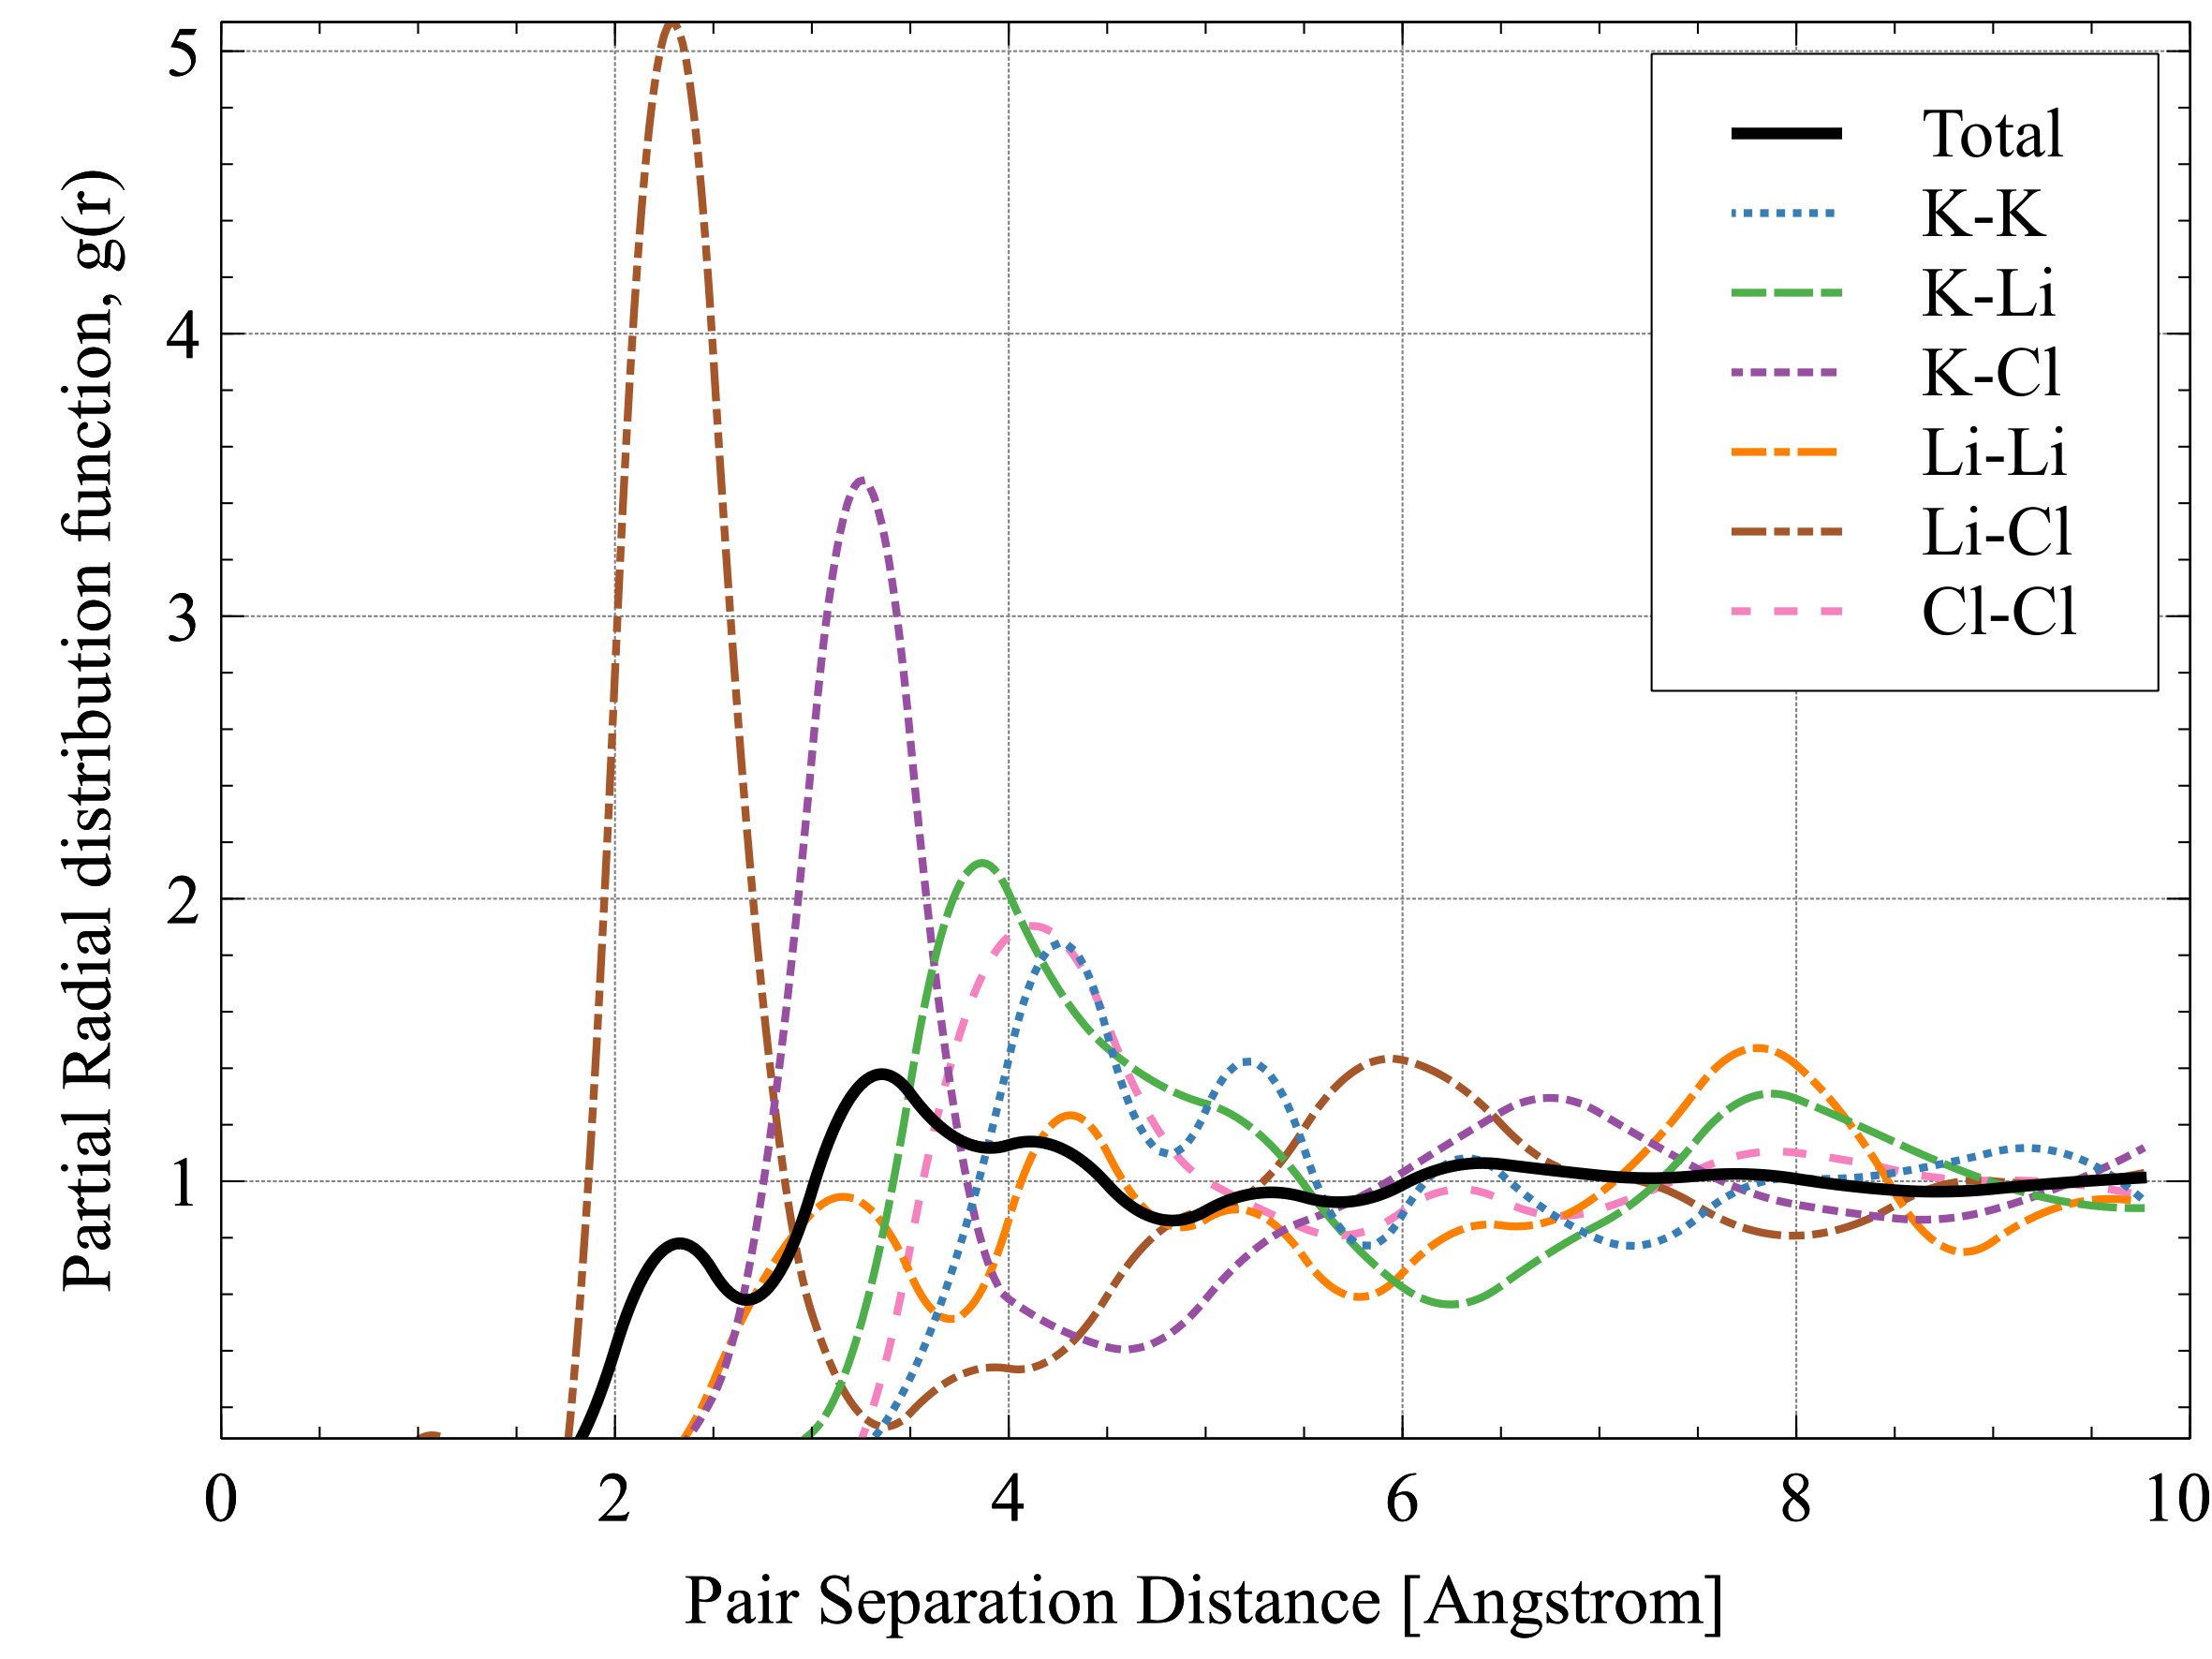
\includegraphics[width=0.8\textwidth]{images/Partial_RDF.jpg} %%%
\DIFdelendFL \DIFaddbeginFL 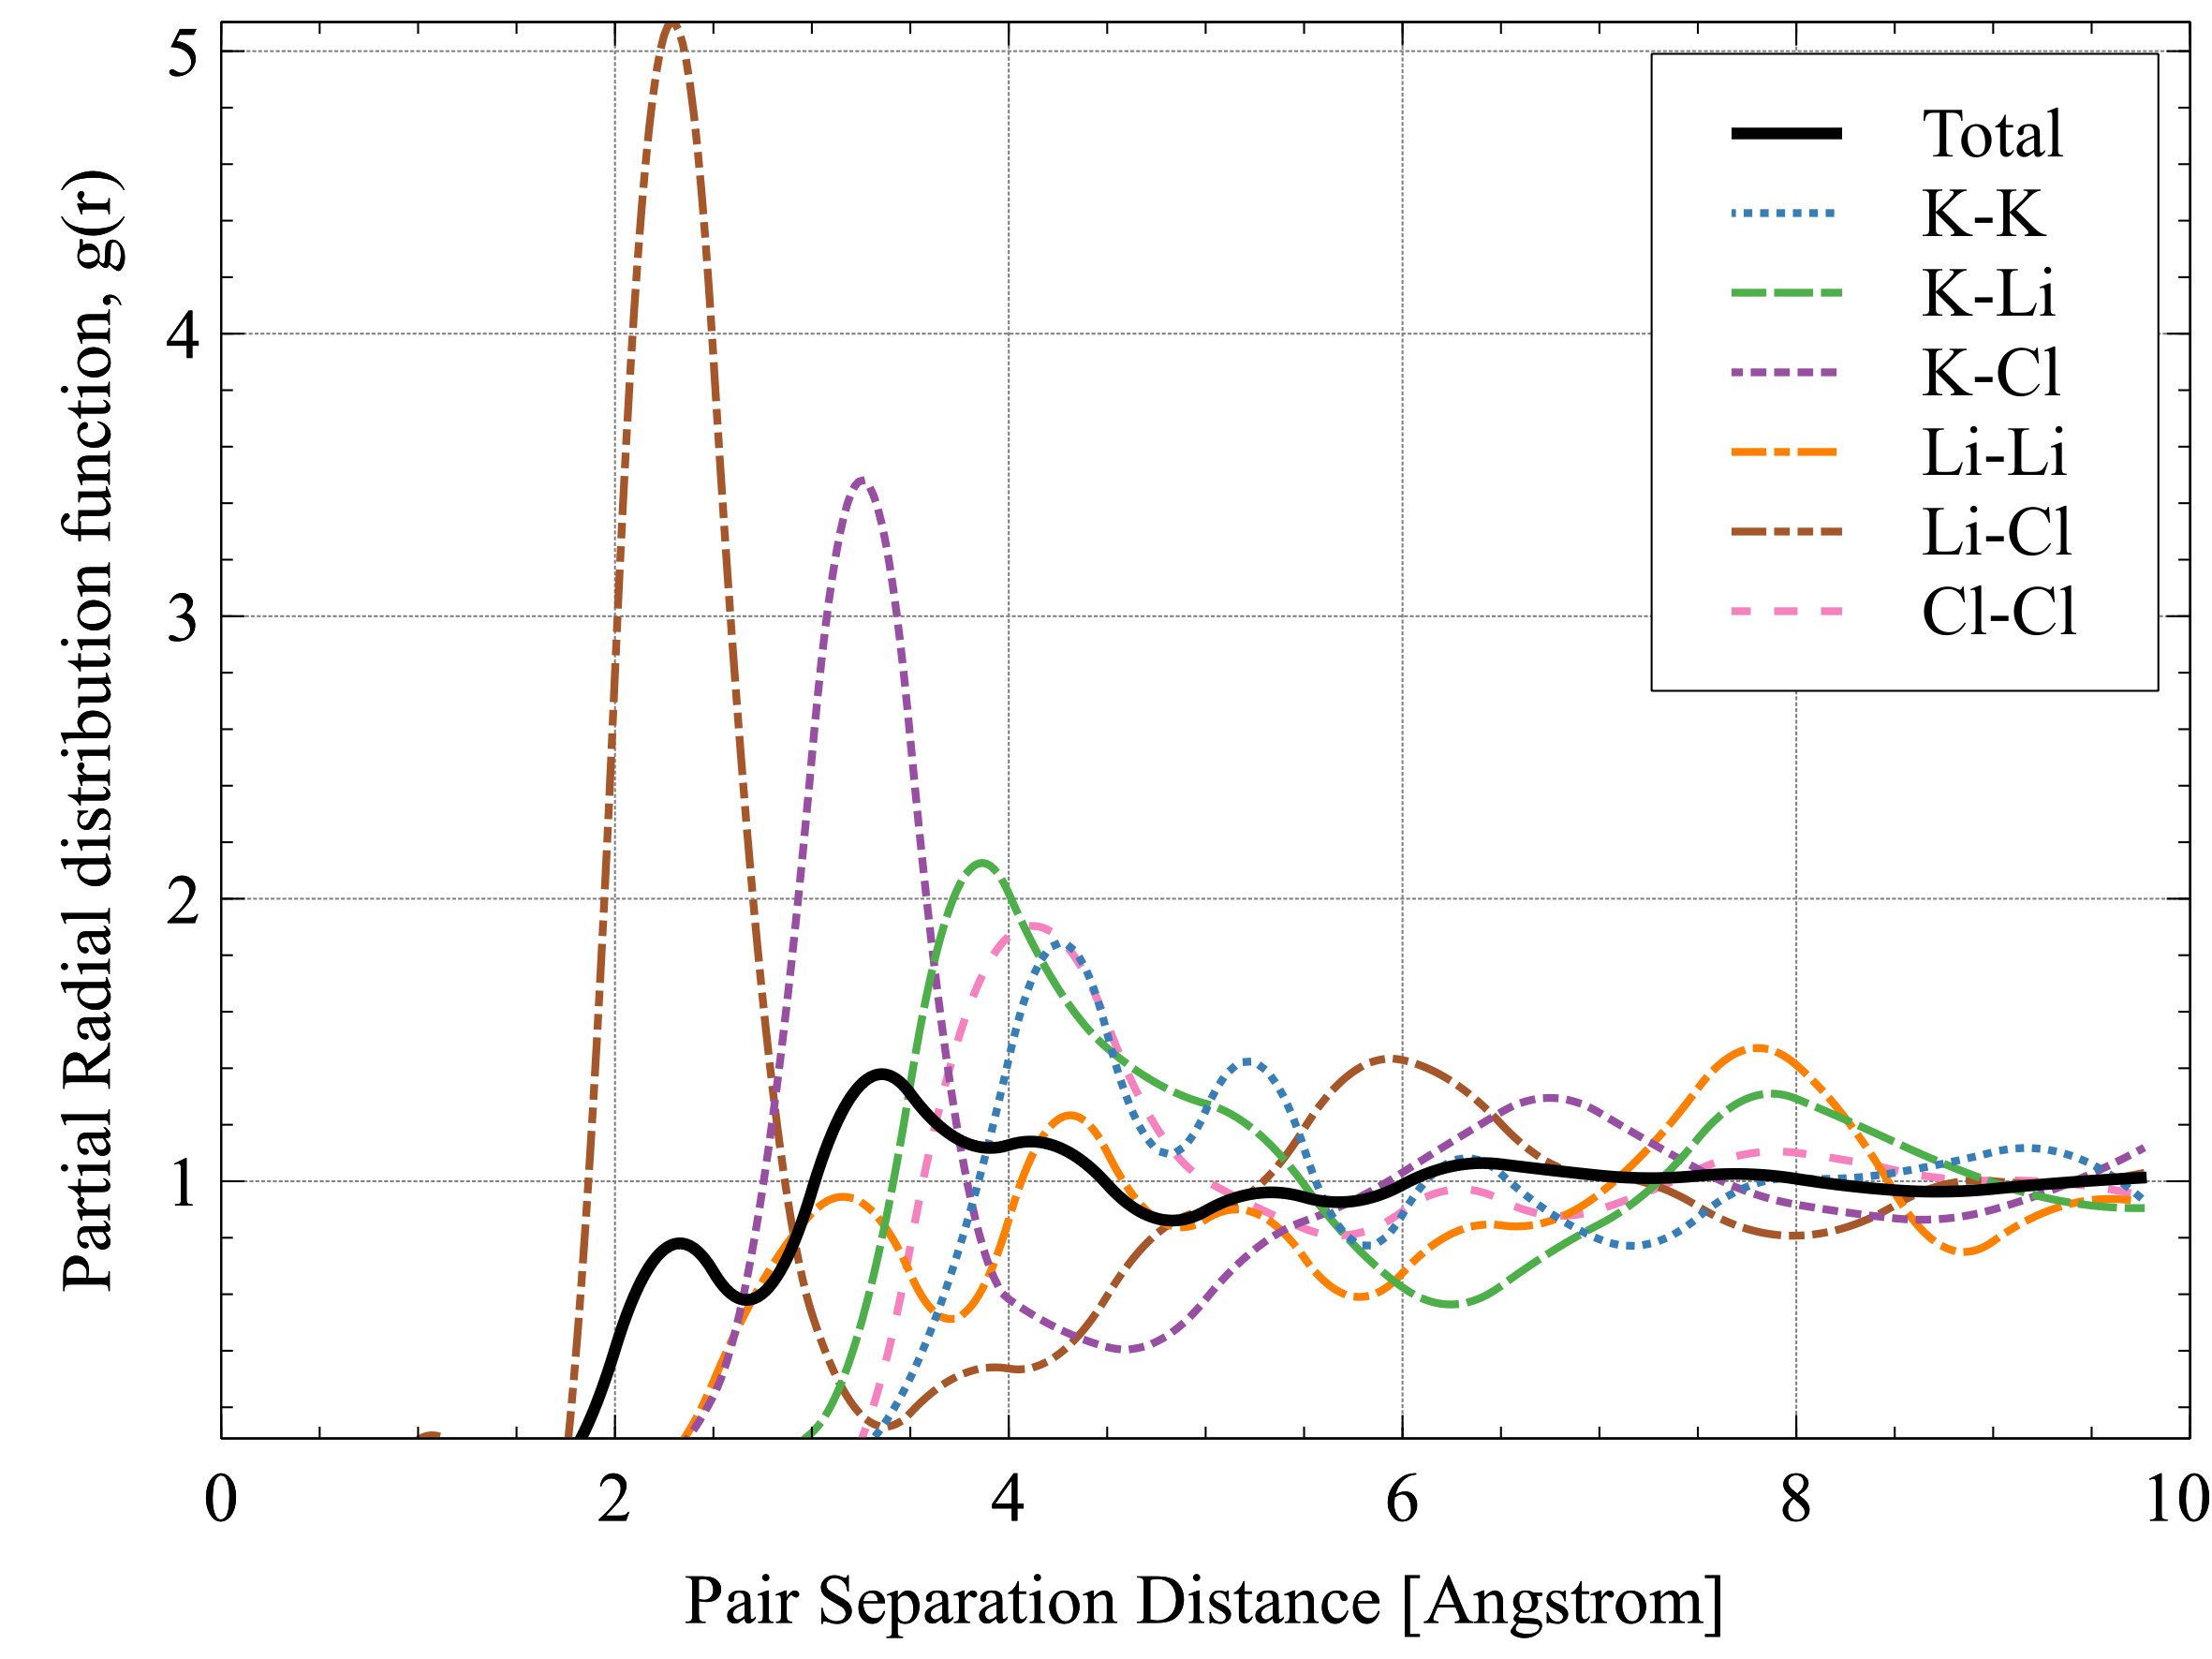
\includegraphics[width=0.7\textwidth]{images/Partial_RDF.jpg} \DIFaddendFL \caption{Snapshot of the partial radial distribution function of liquid \DIFdelbeginFL \DIFdelFL{LiCl-30}\DIFdelendFL \DIFaddbeginFL \DIFaddFL{LiCl-70}\DIFaddendFL \%KCl at \DIFdelbeginFL \DIFdelFL{1300 }\DIFdelendFL \DIFaddbeginFL \DIFaddFL{900 }\DIFaddendFL K.}
 \label{fig:rdf}
 \end{figure}
 Additionally, five unique simulations are performed for each volume to ensure the statistical significance of the results. \DIFaddbegin \DIFadd{The energy at the equilibrium volume is found in the same manner, as the root of the parabolic fit between potential energy and pressure. }\DIFaddend An example of the volume versus pressure relationship is illustrated in Fig. \ref{fig:VvsP} for the 70\% KCl system at 900 K with the standard error of \DIFdelbegin \DIFdel{each data point included shown by error bars . Both this }\DIFdelend \DIFaddbegin \DIFadd{the sample mean pressure shown as the error bars for each unique volume, indicating the statistical certainty of the computed results. Both the }\DIFaddend equilibration procedure and the construction of a pressure-volume curve are conducted for each composition and temperature of interest.

 \begin{figure}[h]
 \centering
 \DIFdelbeginFL %DIFDELCMD < 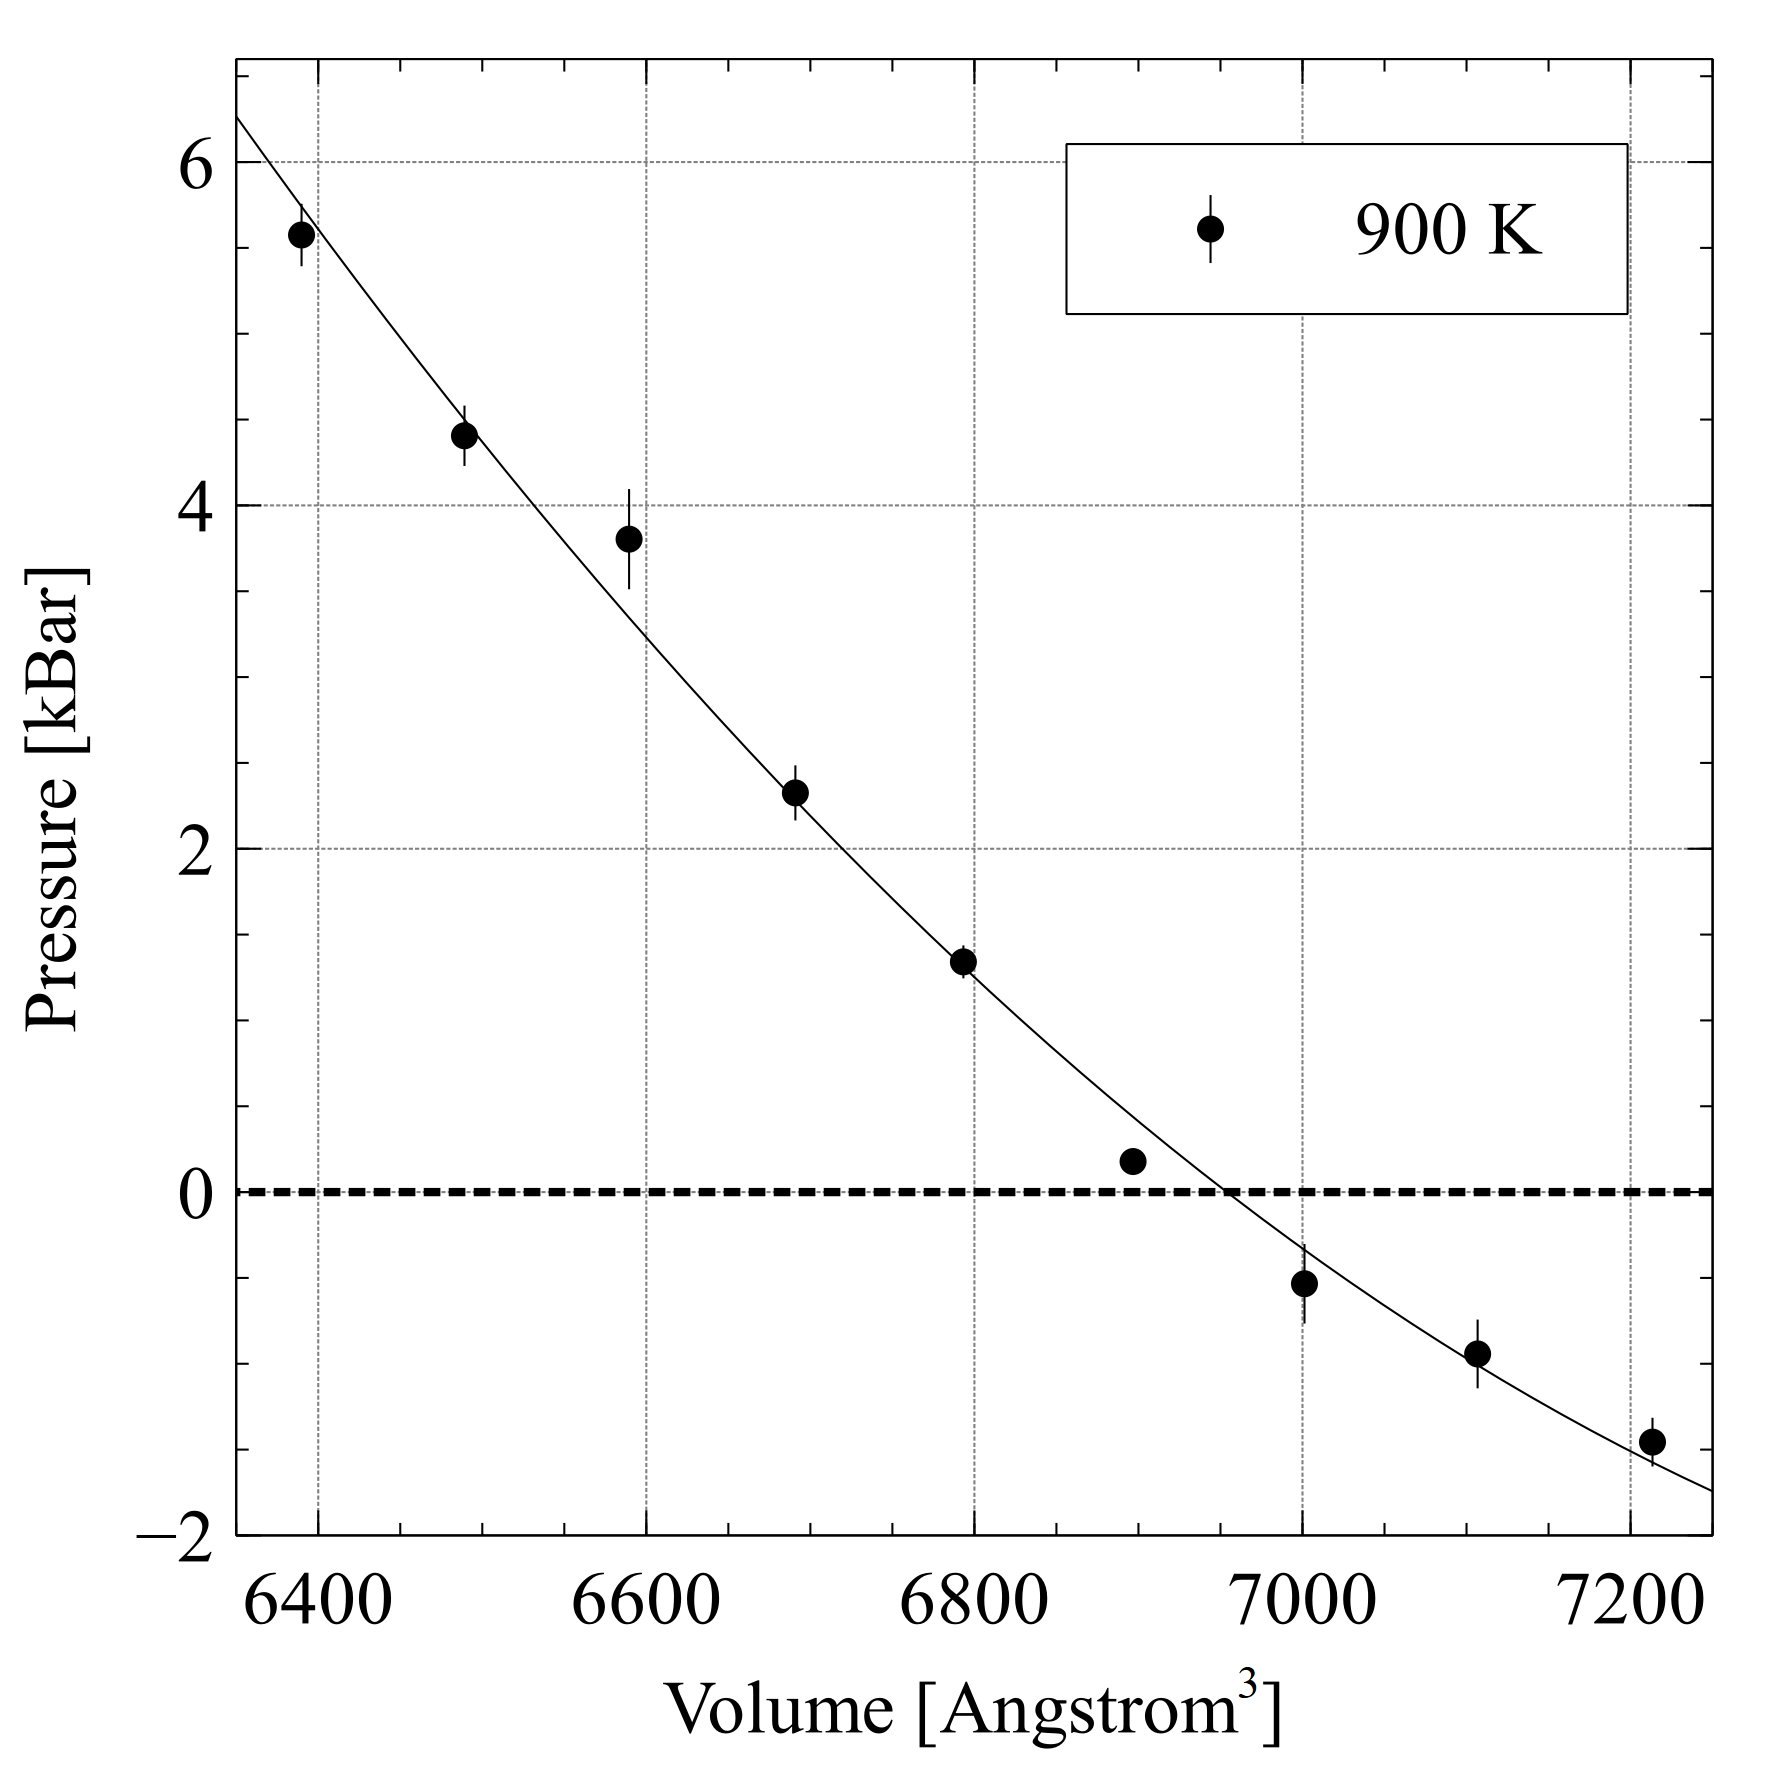
\includegraphics[width=0.8\textwidth]{images/PressureVsVolume.jpg} 
%DIFDELCMD <  %%%
\DIFdelendFL \DIFaddbeginFL 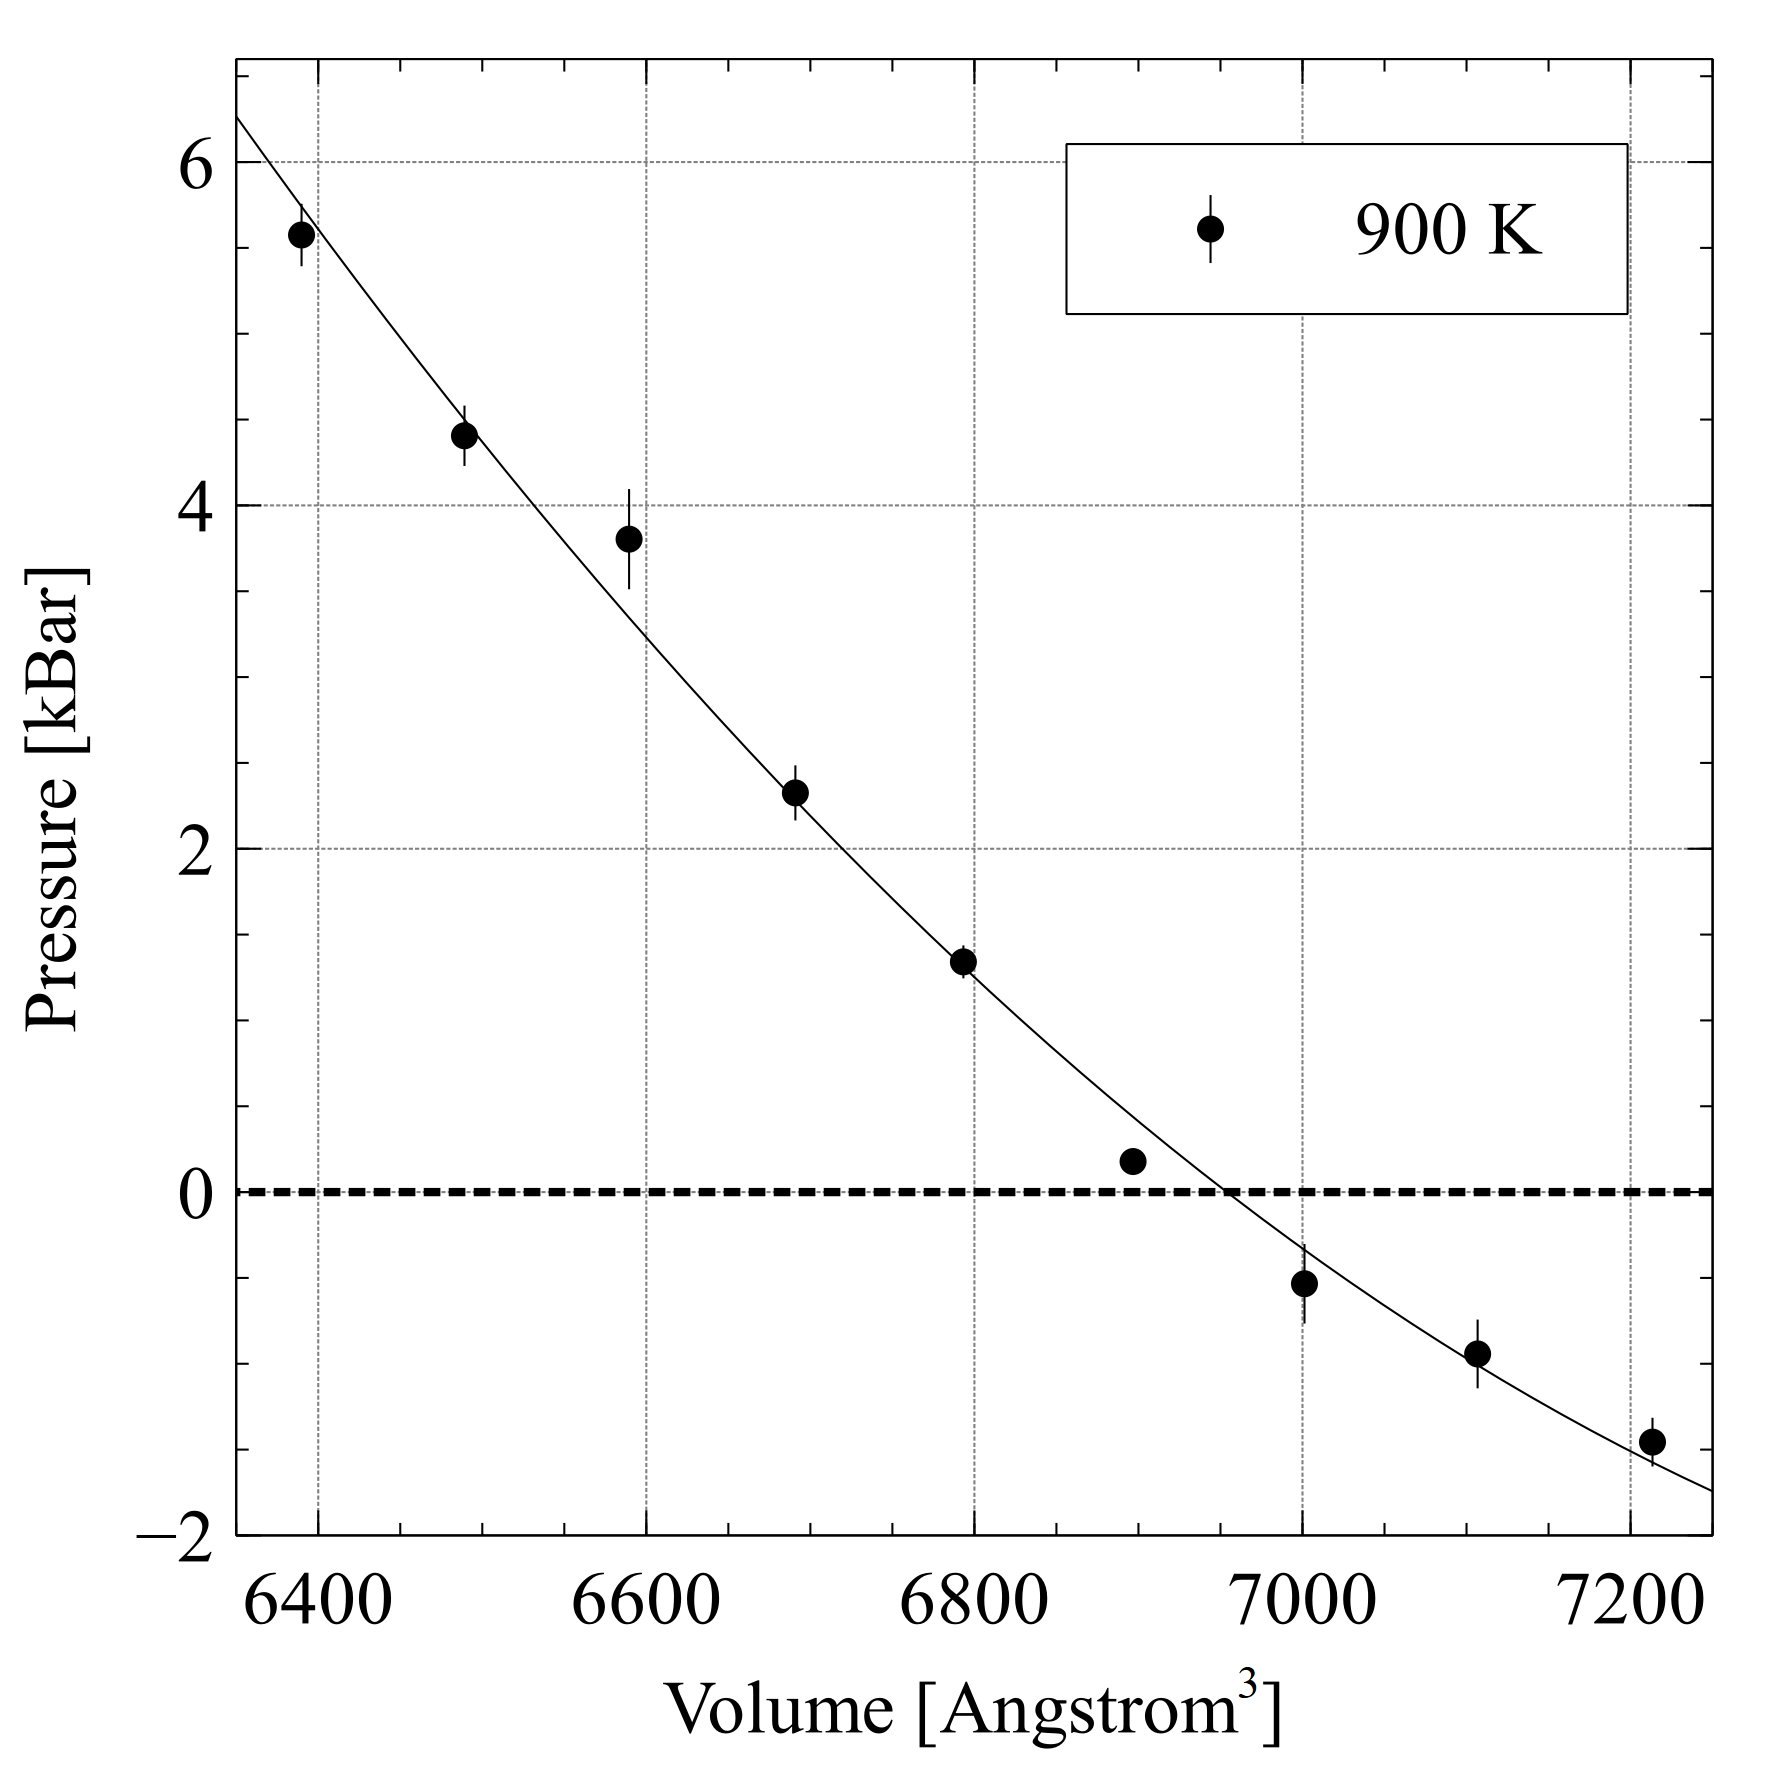
\includegraphics[width=0.7\textwidth]{images/PressureVsVolume.jpg} 
 \DIFaddendFL \caption{Pressure as a function of supercell volume for LiCl-70\%KCl at 900K. The equilibrium volume is the volume at which the pressure is zero. Error bars are standard error \DIFaddbeginFL \DIFaddFL{of sample mean}\DIFaddendFL .}
 \label{fig:VvsP}
\end{figure}

The parabolic fit to the entire data set can be used to calculate the bulk modulus and compressibility of the liquid, as described in equations \ref{eq:bulk modulus} and \ref{eq:compressibility}:

\begin{equation}
\label{eq:bulk modulus}
K = -V {(\frac{dP}{dV})}_{P=0}
\end{equation}

\begin{equation}
\label{eq:compressibility}
\beta = \frac{1}{K}
\end{equation}where K is the bulk modulus, V is the volume, P is the pressure, and $\beta$ is the compressibility. Care was taken to ensure this parabolic fit included at least five unique data points/volumes with at least one data point exhibiting a pressure above 5 kbar, and no data points with a pressure below  -2 kbar. In this manner, a broad and consistent sampling of the pressure-volume space was performed. 

The heat capacity at constant pressure was calculated from equation \ref{eq:Cp}:
\begin{equation}
\label{eq:Cp}
Cp =\lim\DIFdelbegin \DIFdel{_{T\to0} }\DIFdelend \DIFaddbegin \DIFadd{_{\Delta T\to0} }\DIFaddend \frac{dE}{dT}
\end{equation}
where E is the total energy (kinetic plus potential) and T is the absolute temperature. Similar to the \DIFdelbegin \DIFdel{pressure, the total energy }\DIFdelend \DIFaddbegin \DIFadd{equilibrium volume, the pressure }\DIFaddend of the system is tracked as a function of \DIFdelbegin \DIFdel{time and averaged over the final four ps of the simulation. }\DIFdelend \DIFaddbegin \DIFadd{potential energy to find the energy at which the pressure is zero. Then, the kinetic energy is added to determine the total energy. }\DIFaddend The enthalpy of mixing was calculated from the difference in potential energy of the mixture from the two reference molecules. The enthalpy of mixing was normalized by the number of molecules in the system, as in equation \ref{eq:enthalpy}:
\begin{equation}
    \label{eq:enthalpy}
    \Delta H^{mix} = \frac{1}{M}(E_{AB} - x_A E_A - x_B E_B)
\end{equation} 
where $\Delta H^{mix}$ is the enthalpy of mixing per molecule, M is the number of molecules (100 in this case), $E_{AB}$ is the potential energy of LiCl-KCl system, $E_A$ and $E_B$ are the potential energy of two reference systems (LiCl and KCl in this case), and $x_A$ and $x_B$ are the mole fraction for the two respective salts. The Gibbs energy of mixing can also be estimated from the ideal solution model \cite{dehoff2006} at a given temperature by adding an entropy term, as in equation \ref{eq:entropy}: 
\begin{equation}
    \label{eq:entropy}
    -T \Delta S^{mix}= RT[x_A ln x_A + x_B ln x_B]
\end{equation}and incorporating this entropy into  equation \ref{eq:gibbs}:
\begin{equation}
    \label{eq:gibbs}
    \Delta G^{mix} = \Delta H^{mix} -T \Delta S^{mix}
\end{equation}
where $\Delta$ $G_{mix}$ is the Gibbs energy of mixing and R is the gas constant.


\subsection{Experimental Methods}

\DIFaddbegin \subsubsection{\DIFadd{Salt Preparation}}

\DIFadd{The salt mixture preparation was carried out inside an argon atmosphere glovebox (VTI, Model number VTISS1-1809-0100) operated at less than 0.1 ppm H$_{2}$O and O$_{2}$. The LiCl, KCl, and LiCl-KCl eutectic mixture were procured from Sigma Aldrich at $>$99.99\% purity, trace metal basis. The eutectic mixture was used as received. Other compositions 7, 20, 60, 80 and 90 mol\% KCl, were prepared in a glassy carbon crucible (GAT6, 64 mL Sigradur tapered crucible, HTW Germany) in a 40 g batch size. The crucible was cleaned with HPLC grade isopropanol (99.9\% purity, Sigma-Aldrich) prior to use and baked at 800°C under Ar for 8 hours to remove any residual moisture. The LiCl and KCl salts were loaded inside pre-cleaned and baked glassy carbon crucibles in required proportions. Masses were recorded to 0.1 mg precision using a Mettler-Toledo balance (Model number TLE204E). The contents were mixed well and heated to 800 °C for 6 hours using a box furnace (ThermoScientific Thermolyne, Model number FB1315M) inside a glovebox. The salt matrices were allowed to cool and then crushed with agate mortar and pestle for characterization and analysis. ICP-OES was conducted to confirm trace impurity analysis. An explanation of this procedure and detailed results are included in the supplementary information. 
}

\subsubsection{\DIFadd{Density Measurements}} 

\DIFaddend The density of various compositions of LiCl-KCl was measured experimentally using the direct Archimedean method of measuring the buoyancy force exerted on a bobber submerged in the molten salts \cite{Sato2009}. A schematic of the experimental setup \DIFaddbegin \DIFadd{housed inside an inert atmosphere gloevbox }\DIFaddend is shown in Fig. \ref{fig:dens}. A Ni 200 alloy bobber (12.8 mm diameter, 20 mm height) was used for immersion and weight loss determination. A tungsten wire was used for hanging the bobber and a glassy carbon crucible was used to contain salt mixture. \DIFaddbegin \DIFadd{All materials were cleaned using deionized (DI) water and isopropanol and baked at 393 K for 1 hour to remove any residual moisture. Additionally, the glassy carbon crucible was baked at 773 K for 4 hours to remove any adsorbed organic matter. }\DIFaddend A Mettler-Toledo WXTS204 bottom-loading analytical balance (maximum capacity of 220g and precision of 0.1 mg) was used for weight measurements. The density of the salts\DIFaddbegin \DIFadd{, }\DIFaddend $\rho_{salts}$\DIFaddbegin \DIFadd{, }\DIFaddend at an experimental temperature $T$ is calculated by equation \ref{eq:density_exp}:
\begin{equation}
    \label{eq:density_exp}
    \rho_{salts} = \DIFdelbegin \DIFdel{\frac{M_{air} - W_{salts}}{V_0 (1 + 3\alpha(T - T_0))}
}\DIFdelend \DIFaddbegin \DIFadd{\frac{M_{argon} - W_{salts} + \frac{ \pi D\gamma}{g} }{V_0 (1 + 3\alpha(T - T_0))}
}\DIFaddend \end{equation}
where \DIFdelbegin \DIFdel{$M_{air}$ }\DIFdelend \DIFaddbegin \DIFadd{$M_{argon}$ }\DIFaddend is the measured mass of the bobber and wire suspended in \DIFdelbegin \DIFdel{air}\DIFdelend \DIFaddbegin \DIFadd{argon}\DIFaddend , $W_{salts}$ is the measured weight of the bobber and wire suspended in the salts, \DIFaddbegin \DIFadd{$D$ is the diameter of the wire, $\gamma$ is the surface tension of the salts, $g$ is the gravity of Earth, }\DIFaddend $\alpha$ is the linear thermal coefficient of expansion of nickel, and $T_0$ is the reference temperature for the volume of the nickel bobber. The \DIFaddbegin \DIFadd{values of surface tension of the salt were calculated from the two-dimensional equation produced from maximum bubble pressure method measurements \cite{janz1975molten}. The }\DIFaddend volume of the nickel bobber and tungsten wire was first calculated using \DIFdelbegin \DIFdel{deionized }\DIFdelend \DIFaddbegin \DIFadd{DI }\DIFaddend water and ethanol and their known densities near room temperature. This provided the reference volume at 295 K for use with the thermal expansion coefficient to calculate the volume of the bobber at the experimental temperatures. The system was calibrated for high temperature measurements up to 658 K using NaNO$_{3}$ and gave calculated values within 1\% of literature values \DIFdelbegin \DIFdel{were obtained }\DIFdelend \cite{Janz1972}. For measuring the density of each composition of the molten salts at temperatures up to 1111 K, the bobber and wire were first weighed in \DIFdelbegin \DIFdel{air}\DIFdelend \DIFaddbegin \DIFadd{Argon (inside Ar atmosphere glovebox)}\DIFaddend . Then, the salts were melted and the bobber was lowered into the molten salts. \DIFdelbegin \DIFdel{Ten minutes of stable thermal equilibrium was confirmed at }\DIFdelend \DIFaddbegin \DIFadd{At }\DIFaddend each experimental set-point\DIFaddbegin \DIFadd{, the salt was allowed to attain thermal equilibrium for ten minutes, as confirmed }\DIFaddend by a sheathed K-type thermocouple immersed in the salts above the bobber. \DIFdelbegin \DIFdel{After this confirmation of thermal equilibrium }\DIFdelend \DIFaddbegin \DIFadd{Once thermal equilibrium was attained}\DIFaddend , the empty scale was tared and then the weight of the suspended bobber was recorded before the temperature set-point was changed. \DIFaddbegin \DIFadd{This tare and measure method was repeated for a total of three weight measurements at each temperature and the average of these measurements was taken for further density calculation. }\DIFaddend The error of the thermometer ranged from 2.5 to 3.5 K for our experimental temperature range.

\begin{figure}[h]
 \centering
 \DIFdelbeginFL %DIFDELCMD < 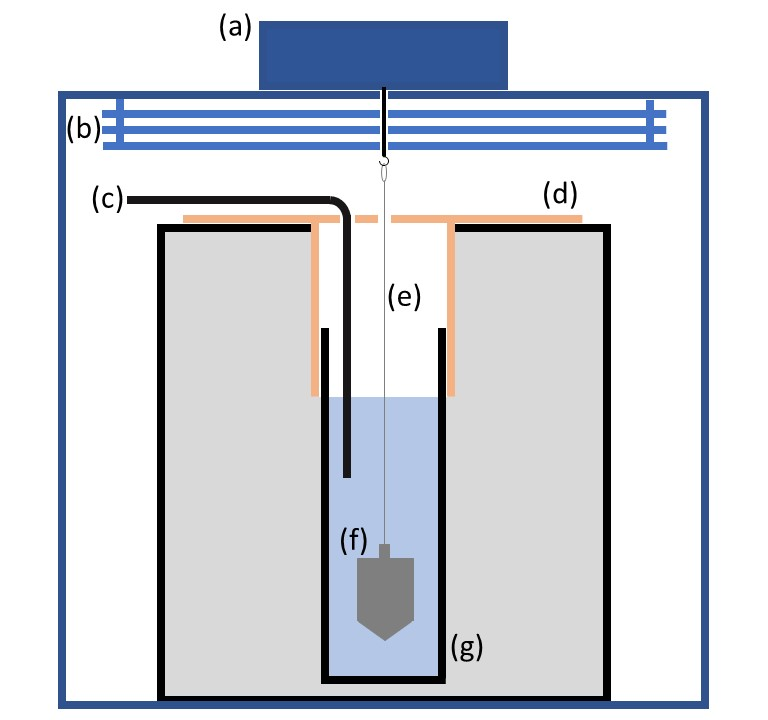
\includegraphics[width=0.5\textwidth]{images/Density_exp_setup.jpg} 
%DIFDELCMD <  %%%
\DIFdelendFL \DIFaddbeginFL 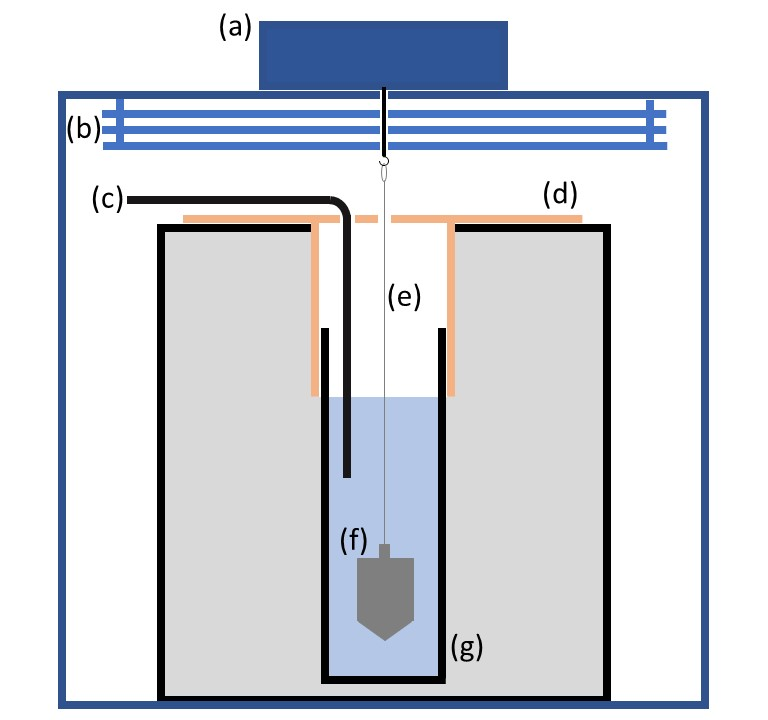
\includegraphics[width=0.7\textwidth]{images/Density_exp_setup.jpg} 
 \DIFaddendFL \caption{Diagram of experimental density setup including (a) balance with bottom hook, (b) heat shields, (c) thermocouple, (d) quartz lid atop furnace, (e) tungsten wire, (f) nickel bobber, and (g) glassy carbon crucible.}
 \label{fig:dens}
\end{figure} 

\DIFaddbegin \subsubsection{\DIFadd{Transition Temperature Analysis}}

\DIFadd{Melt point and transition temperatures were determined for all salt compositions to verify purity of the salt mixtures as well as provide insight into the optimal range for density measurements using a simultaneous thermal analyzer (STA) (Netzsch model STA449F3A-0171-M) and a DSC/TG type S sample carrier. The STA was operated inside an inert argon glove box. An ultra high purity argon protective and purge gas was used, each with a flow rate of 50 ml·min$^{-1}$. Samples were run using a temperature and sensitivity calibration, accurate in the range of 164°C to 950°C, generated using five high purity calibration standards with heating rates of 10 K·min$^{-1}$ and 2 K·min$^{-1}$. The melting temperature and peak area of the standards were calculated by averaging the onset and peak area for three heating cycles. The accuracy of the temperature calibration curve was verified using a silver standard where the experimental melting temperature was 972.0°C, within ±1°C of the reported silver melting temperature of 961.78°C (ASTM E967-18). 
}

\DIFadd{Non-reactive, unsealed glassy carbon crucibles with glassy carbon lids were used for all standards and samples. During data collection and sample preparation, the atmosphere in the glove box had less than 10 ppm O$_2$ and less than 0.1 ppm moisture. 
}


\DIFaddend \FloatBarrier

\section{Results and \DIFdelbegin \DIFdel{Discussion}\DIFdelend \DIFaddbegin \DIFadd{Discussions}\DIFaddend }

\subsection{Down-select of van der Waals dispersion interactions}

The van der Waals (vdW) force plays a fundamental role in determining the structure and properties of ionic liquids. The most common density functionals are unable to correctly describe vdW interactions between atoms and molecules.  There are two common methods to account for vdW interactions within VASP: 1) adding a dispersion correction to the Kohn-Sham energy, or 2) replacing the common exchange-correlation functional with a non-local correlation functional that approximately accounts for dispersion interactions. The most common implementation of the added dispersion correction is from Grimme \cite{Grimme2006,Grimme2010}, in which dispersion coefficients for each atom are tabulated and combined to develop effective pair dispersion coefficients that are dependent upon local geometry. There exist a number of tunable parameters within this implementation that allow for an empirical fitting procedure to try to best approximate the dispersion interactions. For the second option of a replacement functional, Dion et al.\cite{Dion2004} developed a second-order expansion of a quantity contained in the long-range part of the correlation functional, allowing the non-local correlations to be expressed in terms of a density-density interaction formula, and thus seamlessly incorporating vdW forces. There are a number of versions of these vdW functionals available for implementation, and various options available for utilizing the added dispersion term. In literature, a type of vdW interaction is considered and applied, usually without any justification. This work aims to establish a proper interaction implementation for the LiCl-KCl system to best approximate the dispersion interactions/coefficients. 

Seven unique dispersion interactions are employed to investigate the density of the LiCl and KCl systems. These include: 1) the D3 zero damping method with the Perdew-Burke-Ernzerhof (PBE \cite{perdew1996}) exchange-correlation (xc) function (D3-PBE \cite{Grimme2010}); 2) the D3 method with Becke-Jonson (BJ) damping with the PBE xc functional (D3BJ-PBE); 3) the D3 method with zero damping with the revPBE xc functional (D3-rPBE \cite{zhang1998}); 4) the D3 method with Becke-Jonson (BJ) damping with the revPBE xc functional (D3BJ-rPBE); 5) the optB88 functional (optB88 \cite{klimevs2009chemical}); 6) the DF2 functional (DF2 \cite{lee2010}); and 7) the SCAN+rVV10 functional (SCAN \cite{peng2016}). While this is admittedly an incomplete list, this selection incorporates different approaches to accounting for the dispersion interactions. This list also encompasses both commonly utilized methods for describing molten salts, and more recently developed methods that have not been fully explored to describe molten salt systems. 

Following the initialization procedures outlined in the computational methods section (where for this down-select work the initialization was performed with the D3-PBE description), the density \DIFdelbegin \DIFdel{as a function of pressure }\DIFdelend is obtained for both the LiCl and KCl systems at \DIFdelbegin \DIFdel{1100 }\DIFdelend \DIFaddbegin \DIFadd{1000 }\DIFaddend K for each of the seven descriptions investigated. The results are displayed in \DIFdelbegin \DIFdel{Fig. \ref{fig:disp} }\DIFdelend \DIFaddbegin \DIFadd{Table. \ref{tab:my_label} }\DIFaddend and compared to experimental data from Janz \DIFdelbegin \DIFdel{\cite{Janz1988}}\DIFdelend \DIFaddbegin \DIFadd{\cite{janz1975molten,van1955electrical}, which do not contain experimental errors}\DIFaddend . While no description of the LiCl or KCl system matches the experimental data exactly, the three descriptions that come most close (when considering both the LiCl and KCl compositions) are the D3-PBE, D3-rPBE, and the DF2 functional. These three options were further pursued, and intermediate compositions of LiCl-20KCl, LiCl-41KCl, and LiCl-80KCl were explored. \DIFaddbegin \DIFadd{SCAN is excluded from the KCl data as the predictions were far outside the expected bounds and not pursued further.
 }\DIFaddend 


\DIFdelbegin %DIFDELCMD < \begin{figure}[h]
%DIFDELCMD <  %%%
\DIFdelendFL \DIFaddbeginFL \begin{table}[]
    \DIFaddendFL \centering
    \DIFdelbeginFL %DIFDELCMD < 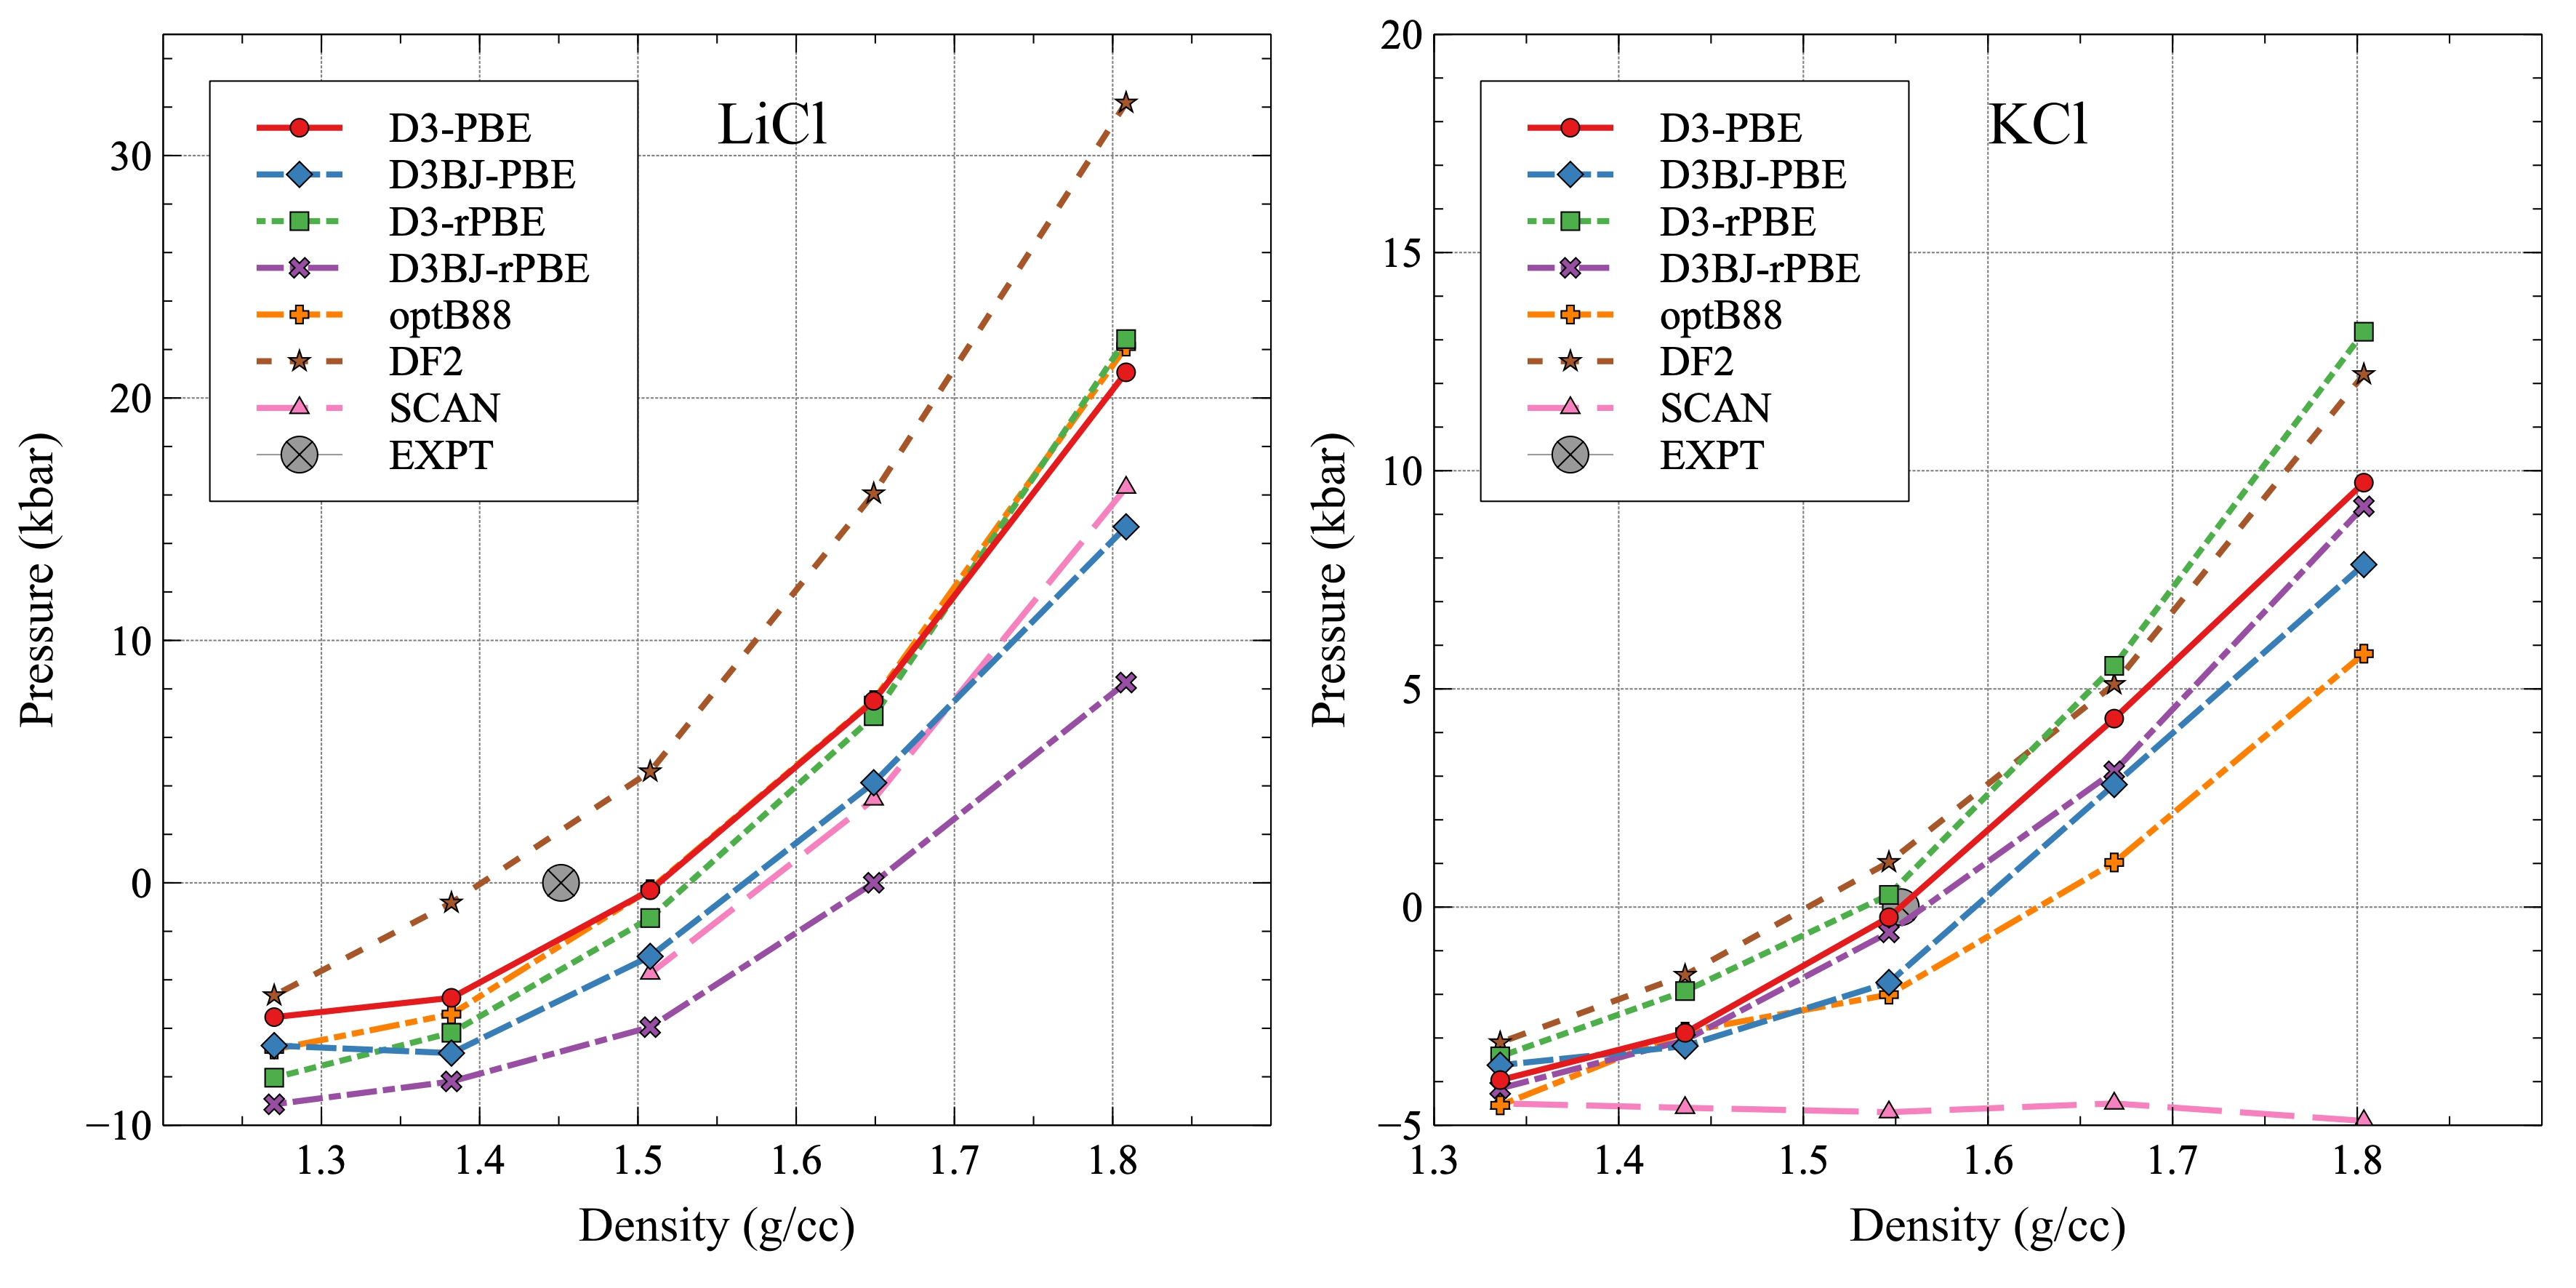
\includegraphics[width=\textwidth]{images/LiClKCl_disp.jpg} 
%DIFDELCMD <  %%%
\DIFdelendFL \DIFaddbeginFL \begin{tabular}{|c|c|c|c|c|}
\hline
\DIFaddFL{Method	}&	\DIFaddFL{LiCl	}& \DIFaddFL{Percent Difference }&	\DIFaddFL{KCl }& \DIFaddFL{Percent Difference	}\\
\hline
\DIFaddFL{EXPT	}&	\DIFaddFL{1.451	}& \DIFaddFL{-}&	\DIFaddFL{1.553 }&\DIFaddFL{-	}\\
\DIFaddFL{D3-PBE	}&	\DIFaddFL{1.513	}& \DIFaddFL{4.27}&	\DIFaddFL{1.553 }& \DIFaddFL{0	}\\
\DIFaddFL{D3BJ-PBE	}&	\DIFaddFL{1.568 }&	\DIFaddFL{8.06}&	\DIFaddFL{1.593 }& \DIFaddFL{2.58	}\\
\DIFaddFL{D3-rPBE	}&	\DIFaddFL{1.532	}& \DIFaddFL{5.58}&	\DIFaddFL{1.532 }& \DIFaddFL{1.35	}\\
\DIFaddFL{D3BJ-rPBE	}&	\DIFaddFL{1.649 }&	\DIFaddFL{13.65}&	\DIFaddFL{1.566 }& \DIFaddFL{0.84	}\\
\DIFaddFL{optB88	}&	\DIFaddFL{1.512	}& \DIFaddFL{4.20}&	\DIFaddFL{1.627 }& \DIFaddFL{4.76	}\\
\DIFaddFL{DF2	}&	\DIFaddFL{1.401	}& \DIFaddFL{3.45}&	\DIFaddFL{1.502 }& \DIFaddFL{3.28	}\\
\DIFaddFL{SCAN }& \DIFaddFL{1.581 }& \DIFaddFL{8.96}& \DIFaddFL{-}&\DIFaddFL{- }\\
\hline
    \end{tabular}
    \DIFaddendFL \caption{The density \DIFdelbeginFL \DIFdelFL{as a function of }\DIFdelendFL \DIFaddbeginFL \DIFaddFL{(g/cc) and percent difference (\%) at zero }\DIFaddendFL pressure at \DIFdelbeginFL \DIFdelFL{1100 }\DIFdelendFL \DIFaddbeginFL \DIFaddFL{1000 }\DIFaddendFL K for LiCl and KCl utilizing seven unique descriptions for the vdW forces, compared to experimental data from Janz \DIFdelbeginFL \DIFdelFL{\cite{Janz1988}}\DIFdelendFL \DIFaddbeginFL \DIFaddFL{\cite{janz1975molten,van1955electrical}}\DIFaddendFL . }
    \DIFdelbeginFL %DIFDELCMD < \label{fig:disp}
%DIFDELCMD < \end{figure} 
%DIFDELCMD < %%%
\DIFdelend \DIFaddbegin \label{tab:my_label}
\end{table}
\DIFaddend 


The results for the density of the LiCl-KCl system as a function of composition for three unique dispersion relationships are shown in Fig. \ref{fig:disp_tot}. Again, it is emphasized that none of the three best dispersion interactions can exactly replicate the experimental density from Janz as a function of composition for this pseudo-binary system. The \DIFdelbegin \DIFdel{relative error changes depending upon the composition for each description, introducing difficulties in determining the appropriate dispersion interaction with which to proceed. The total error over the five compositions is minimized for the D3-PBE dispersion interaction, however, the trend of density as a function of composition is most closely mirrored by the DF2 functional. Considering that this work has an emphasis on a broad range of compositions and temperatures, it was deemed that obtaining the correct trends in the density as a function of composition was more important than most closely matching the experimental density for a few compositions. Thus, the DF2 functional was chosen to pursue the full description of the thermophysical properties of the LiCl-KCl system. 
}\DIFdelend \DIFaddbegin \DIFadd{density data from Janz does not provide the experimental error but is expected to be on the order of 1\%DIF > . The relative error changes depending upon the composition for each description, introducing difficulties in determining the appropriate dispersion interaction with which to proceed. The total error over the five compositions is minimized for the D3-PBE dispersion interaction, however, the trend of density as a function of composition is most closely mirrored by the DF2 functional. Considering that this work has an emphasis on a broad range of compositions and temperatures, it was deemed that obtaining the correct trends in the density as a function of composition was more important than most closely matching the experimental density for a few compositions. Thus, the DF2 functional was chosen to pursue the full description of the thermophysical properties of the LiCl-KCl system. 
}\DIFaddend 

\begin{figure}[h]
 \centering
 \DIFdelbeginFL %DIFDELCMD < 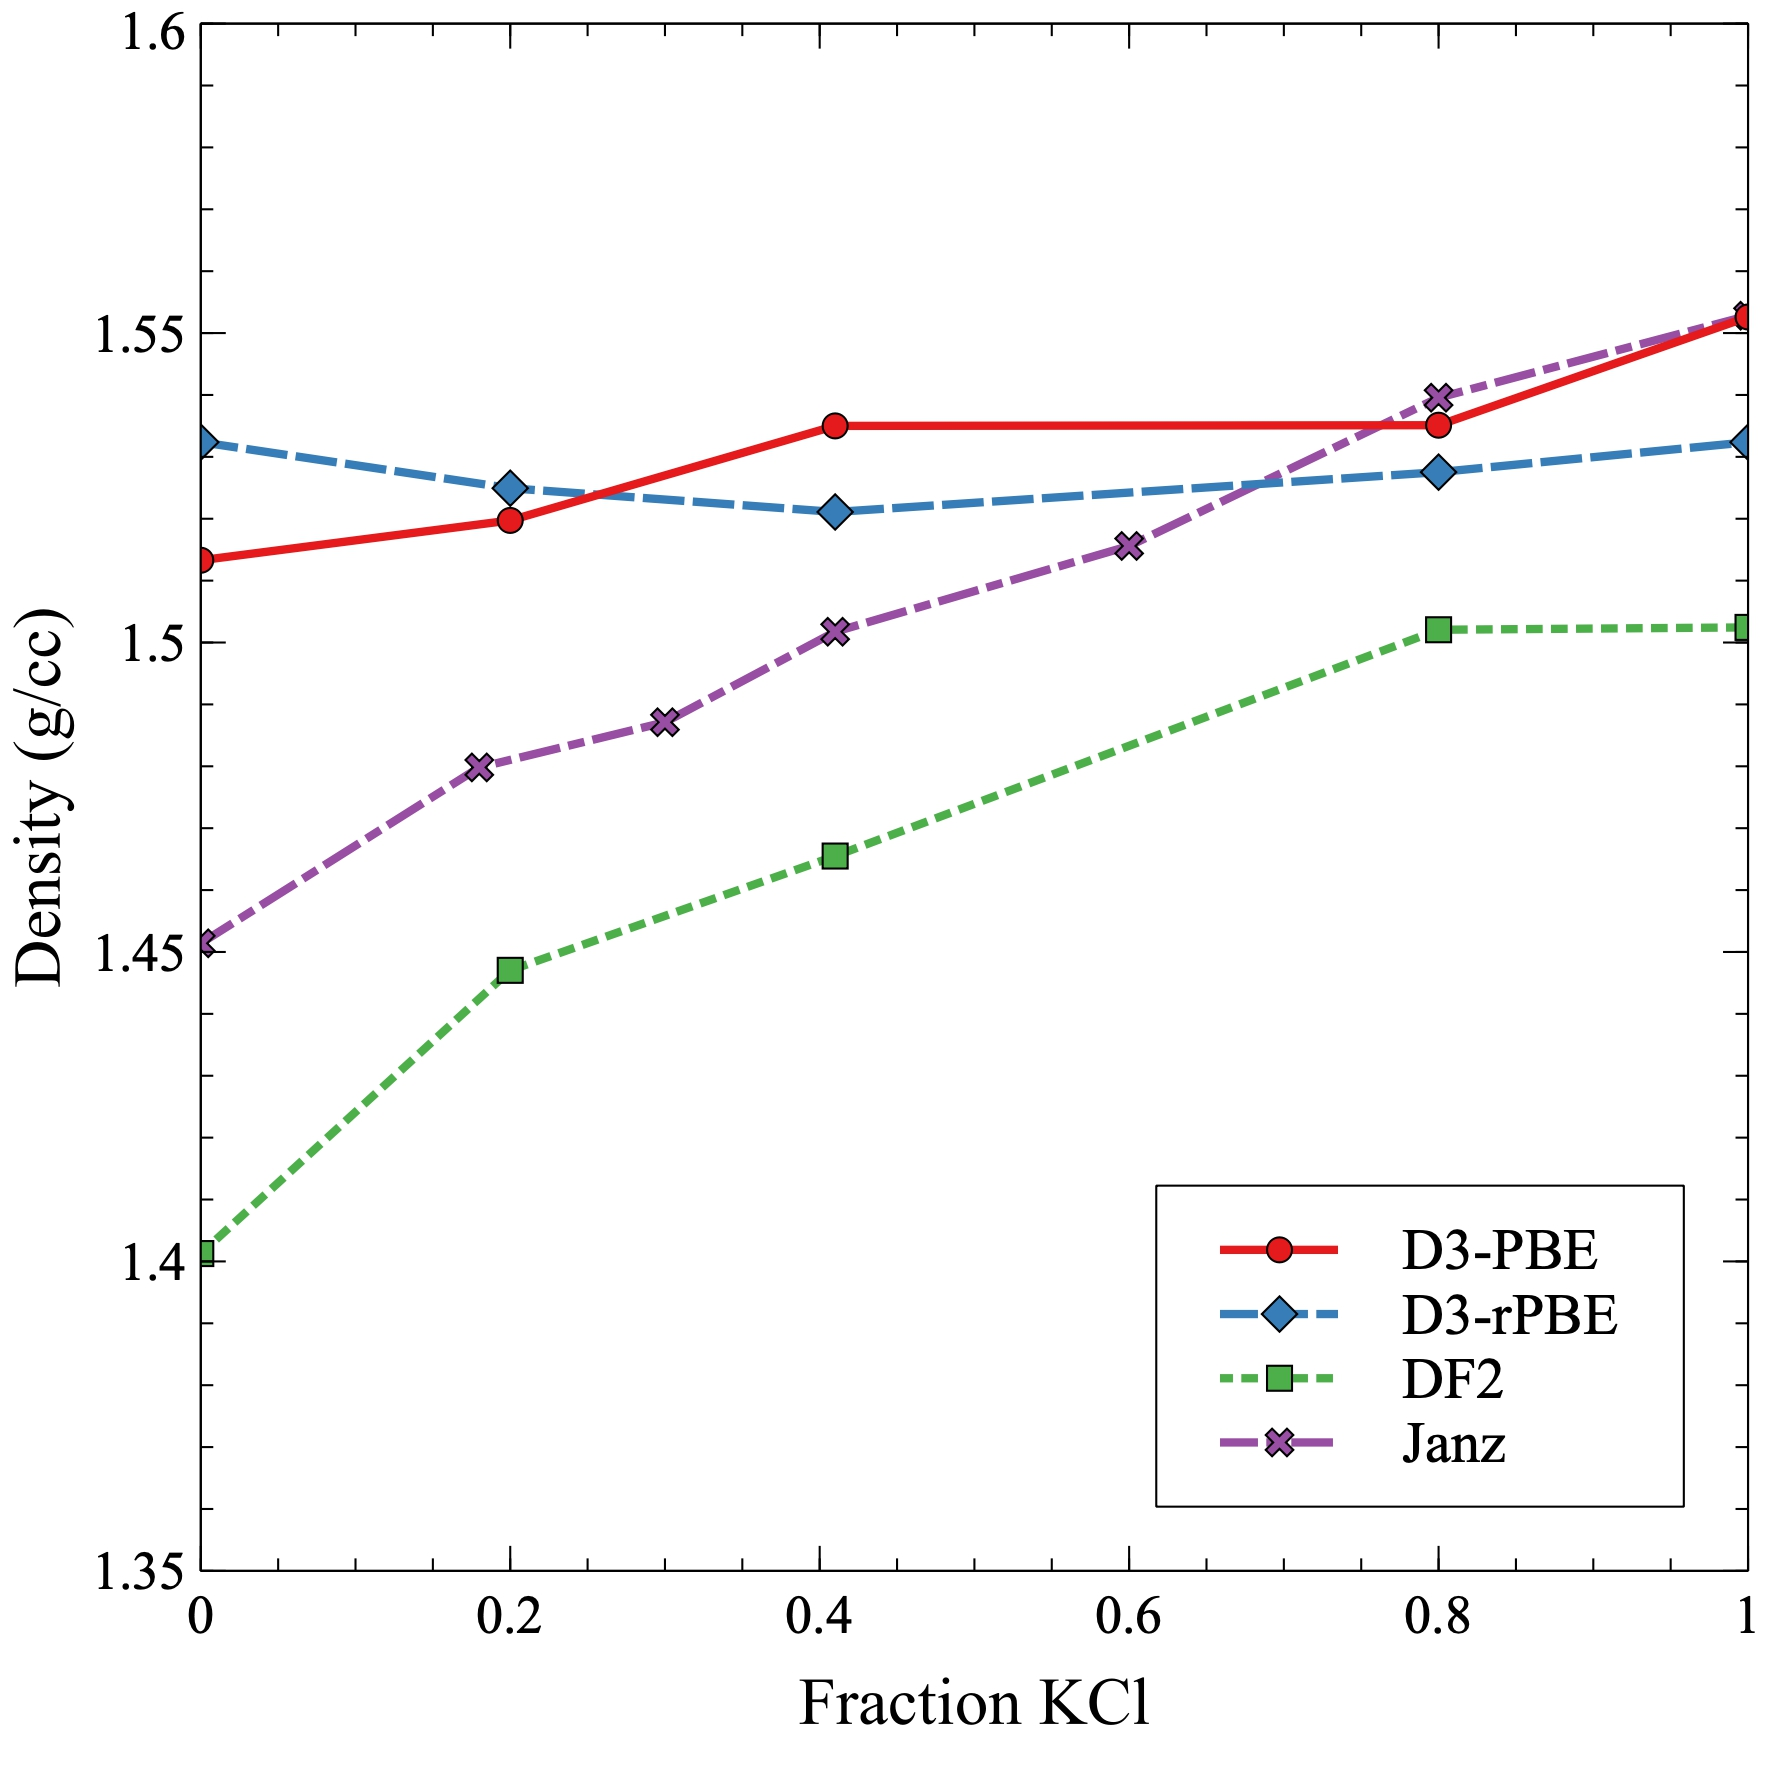
\includegraphics[width=0.6\textwidth]{images/final_disp.jpg} 
%DIFDELCMD <  %%%
\DIFdelendFL \DIFaddbeginFL 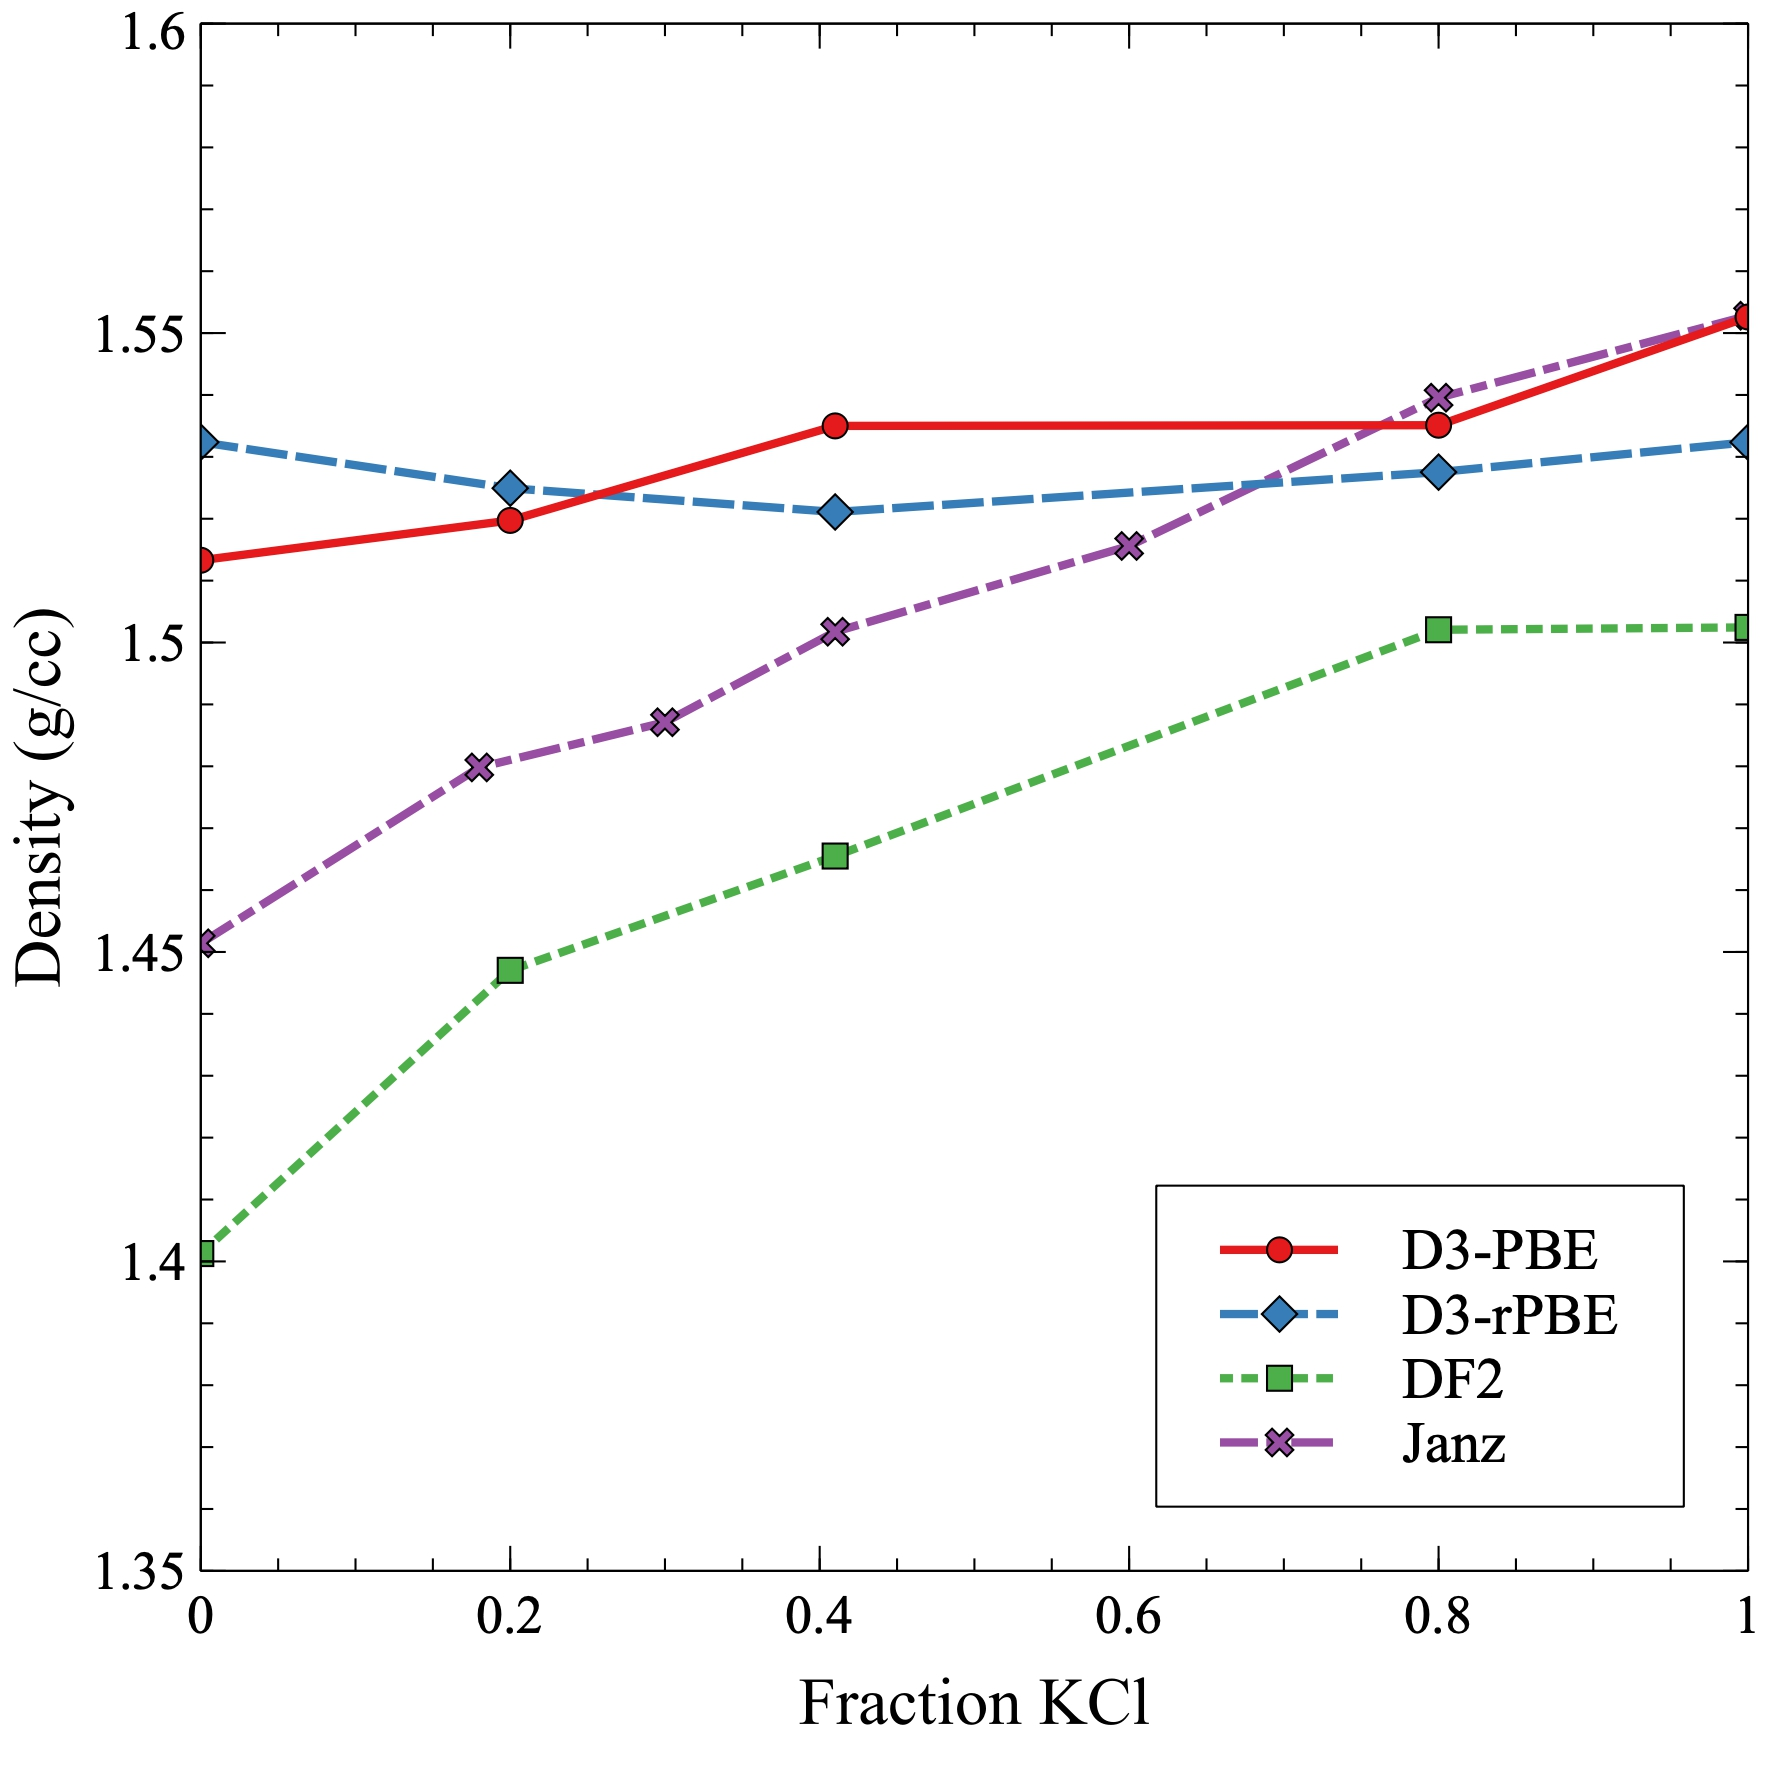
\includegraphics[width=0.7\textwidth]{images/final_disp.jpg} 
 \DIFaddendFL \caption{The density as a function of pressure at \DIFdelbeginFL \DIFdelFL{1100 }\DIFdelendFL \DIFaddbeginFL \DIFaddFL{1000 }\DIFaddendFL K for at five select compositions in the LiCl-KCl utilizing the three best descriptions for the vdW forces, compared to experimental data from Janz \DIFdelbeginFL \DIFdelFL{\cite{Janz1988}.}\DIFdelendFL \DIFaddbeginFL \DIFaddFL{\cite{janz1975molten,van1955electrical}}\DIFaddendFL }
 \label{fig:disp_tot}
\end{figure} 

It should be noted that in the down-select work, only a single simulation is performed for each specific volume and dispersion interaction. This increases the uncertainty in the reported data within this section, but the calculated density is not expected to vary by more than 1-2\%. Such magnitudes of error do not alter the gained understanding of the relative performance of the individual dispersion descriptions. For the most accurate description of thermophysical properties, please refer to the below sections. 

\FloatBarrier

\subsection{Computational Results}

The density as a function of composition for each temperature is shown in Fig. \ref{fig:density}A, with a comparison to selected literature values at \DIFdelbegin \DIFdel{1100 }\DIFdelend \DIFaddbegin \DIFadd{1200 }\DIFaddend K in Fig. \ref{fig:density}B. Second order polynomial fits to each complete data set are shown as lines. Data below 1000 K is not considered "complete" in this context because data for all compositions was not collected. This is because individual compositions of LiCl-KCl would be expected to be solid at these temperatures and this study only included the liquid phase. The calculated densities nearly exactly match the experimental data collected by \DIFdelbegin \DIFdel{Wang et al. \cite{Wang2015}, but are slightly below the values calculated by }\DIFdelend Janz et al. \DIFdelbegin \DIFdel{\cite{Janz1988}. However, this discrepancy with Janz deceases as the concentration of KCl increases. The density tends to increase as a function of KCl, exhibiting slightly positive deviations from linearity. As expected, the density decreases with increasing temperature.  Finally, a comparison can be made to the Born-Mayer-Huggins interatomic potential employed in the classical molecular simulations by Wang et al. \cite{Wang2015}, which significantly underestimates the equilibrium density across the entire compositional range.This validates the use of DFT with vdW-DF2 van der Waals functional for the calculation of density in molten salt systems.
}\DIFdelend \DIFaddbegin \DIFadd{\cite{janz1975molten,van1955electrical}. The density data from Janz does not provide the experimental error but is expected to be on the order of 1\%. The density tends to increase as a function of KCl, exhibiting slightly positive deviations from linearity. As expected, the density decreases with increasing temperature.  
}\DIFaddend 

\begin{figure}[h]
 \centering
 \DIFdelbeginFL %DIFDELCMD < 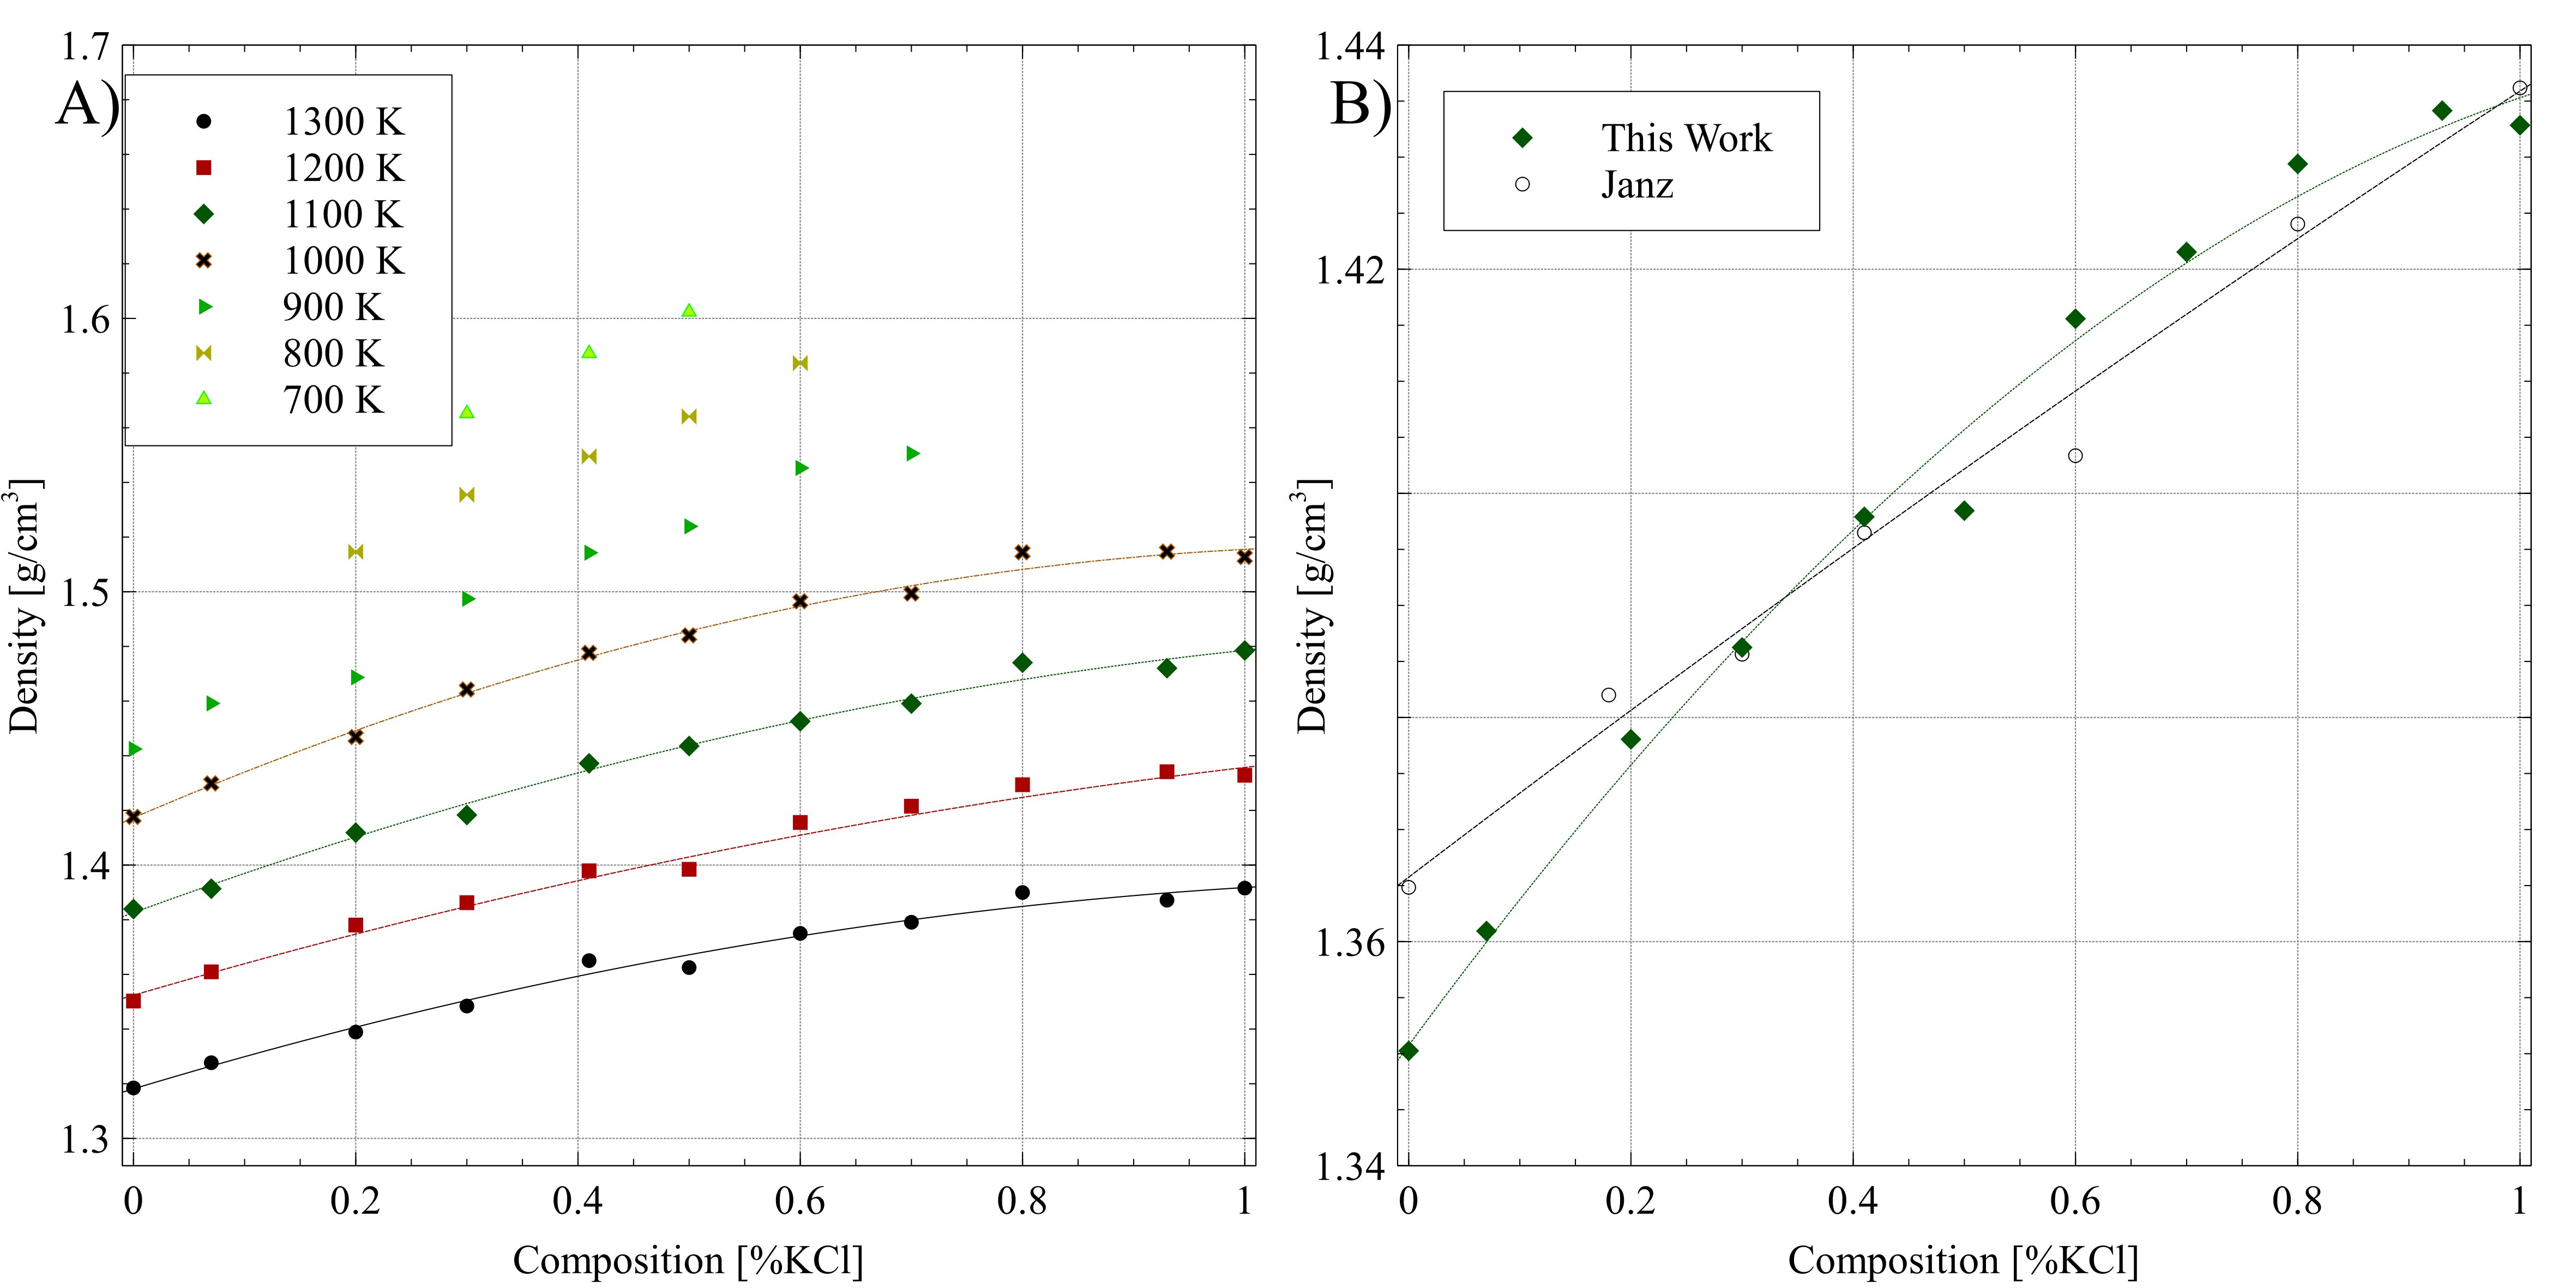
\includegraphics[width=0.8\textwidth]{images/denisty_combined_figures.jpg} 
%DIFDELCMD <  %%%
\DIFdelendFL \DIFaddbeginFL 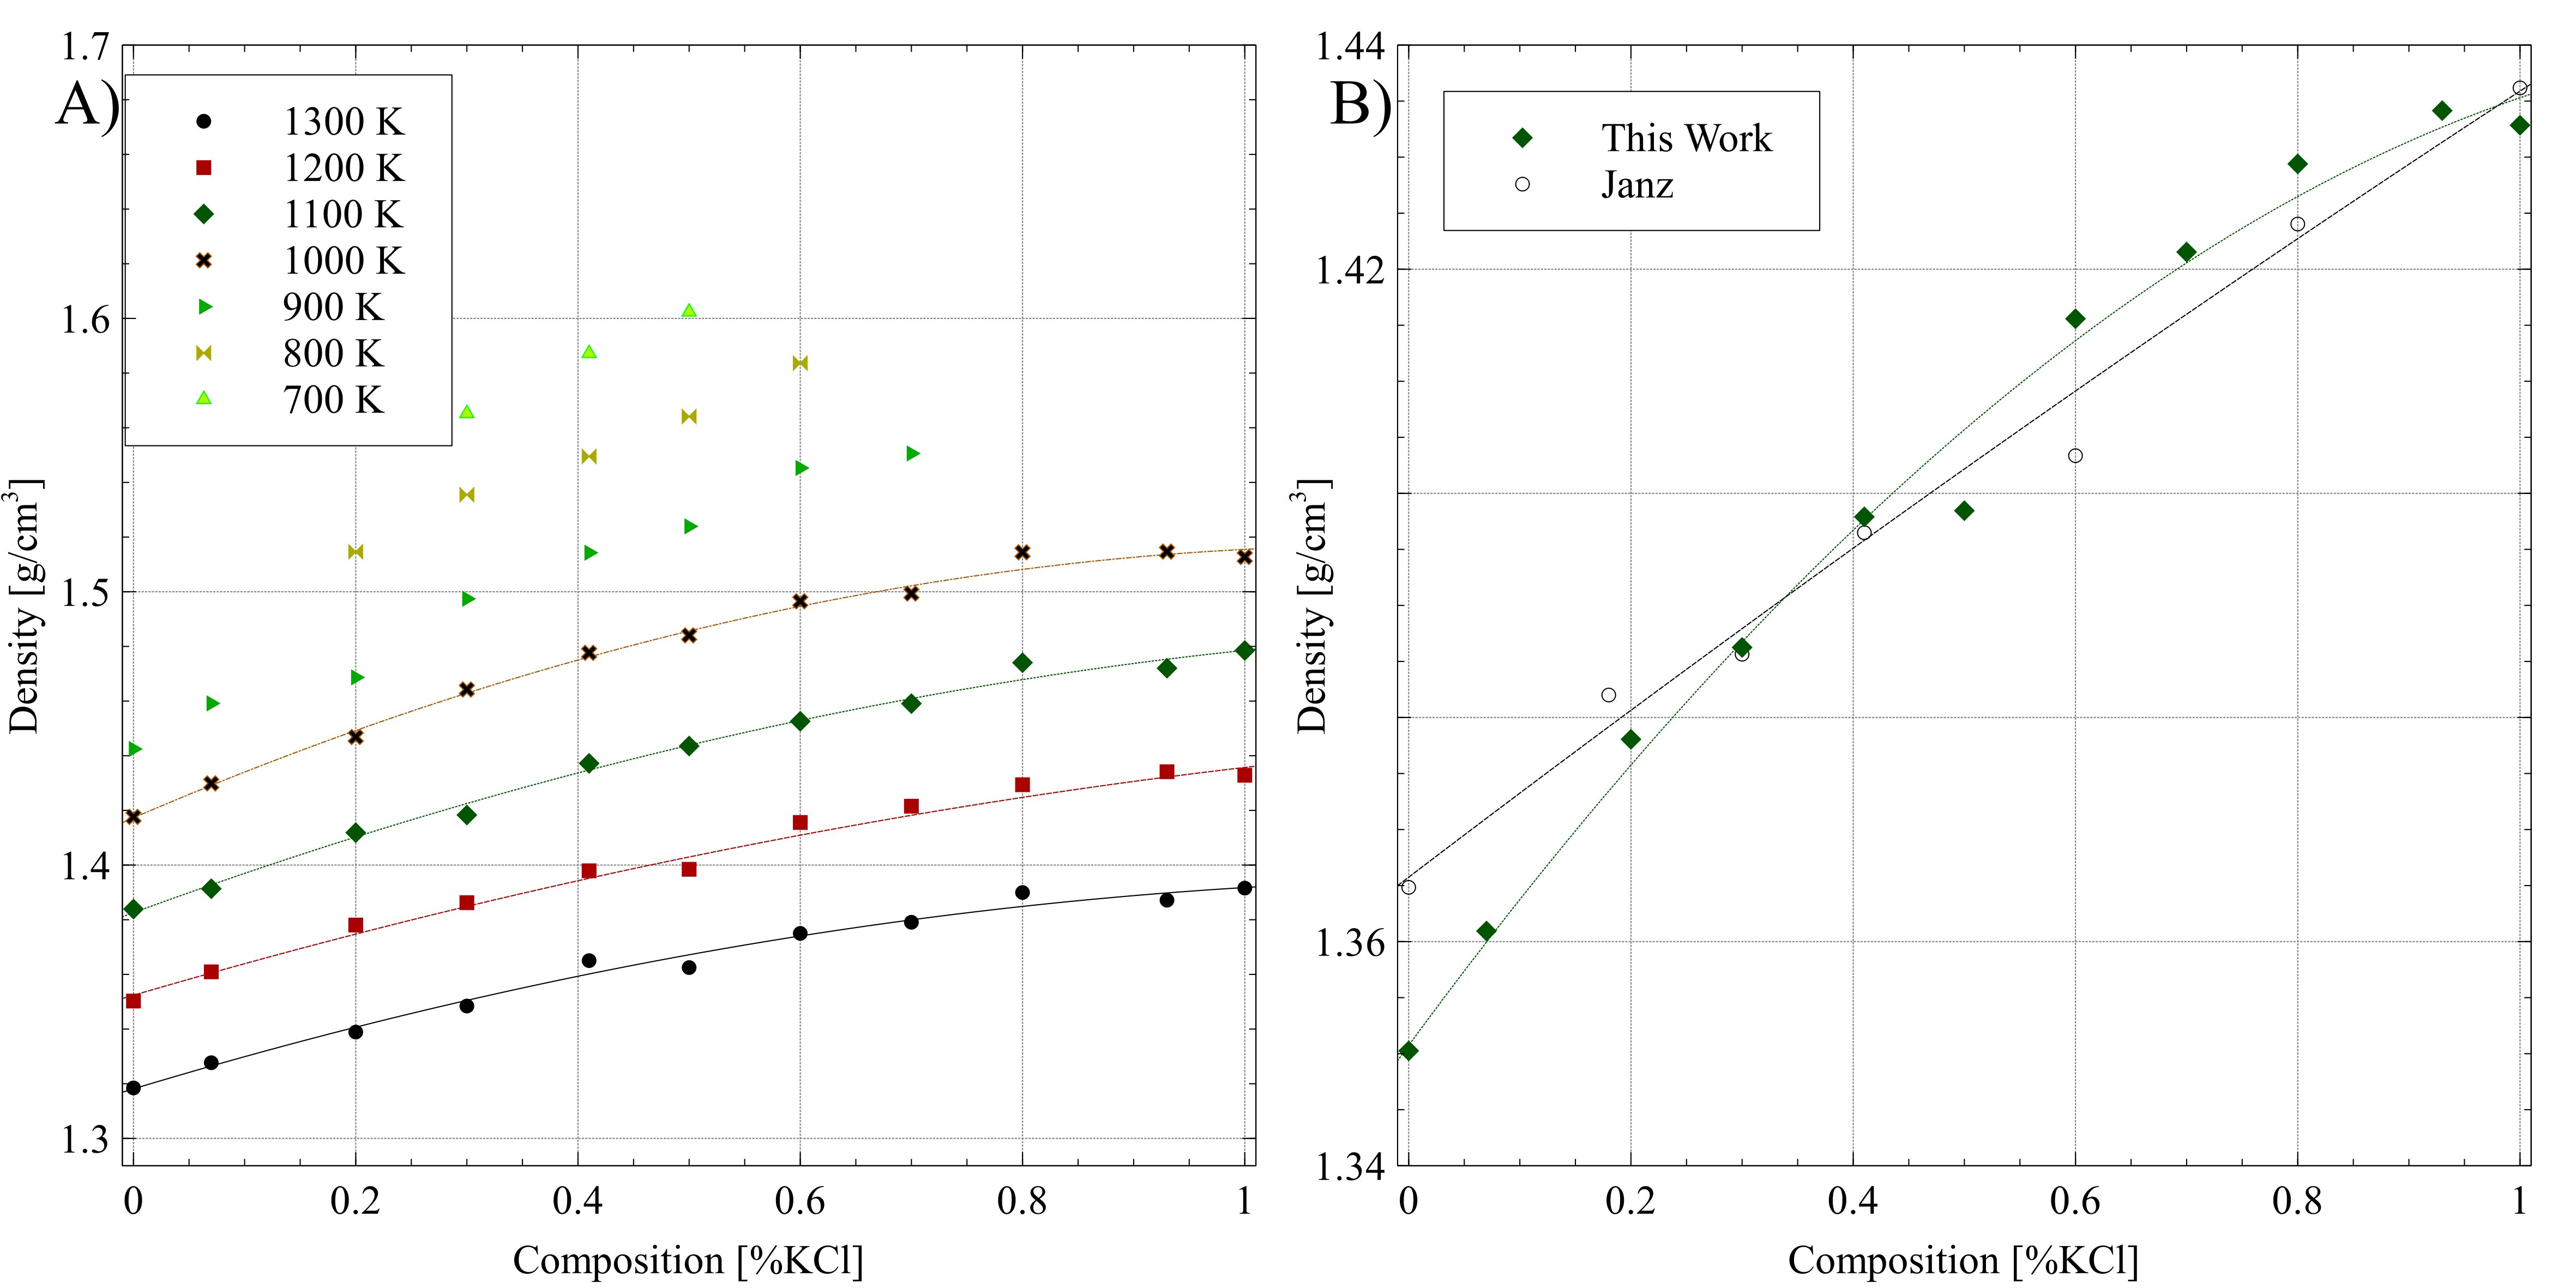
\includegraphics[width=1.0\textwidth]{images/denisty_combined_figures.jpg} 
 \DIFaddendFL \caption{In A) the density of LiCl-KCl system as a function of composition. In B) the density of LiCl-KCl system as a function of composition at \DIFdelbeginFL \DIFdelFL{1100 }\DIFdelendFL \DIFaddbeginFL \DIFaddFL{1200 }\DIFaddendFL K. Filled markers are computational and open are experimental. AIMD results are compared to \DIFdelbeginFL \DIFdelFL{classical molecular dynamics and }\DIFdelendFL experimental results from \DIFdelbeginFL \DIFdelFL{Wang et al. \cite{Wang2015}, and experimental results from }\DIFdelendFL Janz et al. \DIFdelbeginFL \DIFdelFL{\cite{Janz1988} }\DIFdelendFL \DIFaddbeginFL \DIFaddFL{\cite{janz1975molten,van1955electrical} }\DIFaddendFL are at \DIFdelbeginFL \DIFdelFL{1100K}\DIFdelendFL \DIFaddbeginFL \DIFaddFL{1200K}\DIFaddendFL . Second order polynomial fits to each complete data set are shown as lines.}
 \label{fig:density}
\end{figure} 


\FloatBarrier

The compressibility as a function of composition and temperature is shown in Fig. \ref{fig:compressibility}. \DIFaddbegin \DIFadd{The linear fits were only intended to be used to illustrate overall trends of the data and not to suggest that a linear fit most appropriately suits the data. }\DIFaddend This data displays significantly greater scatter than the density, however, general trends can still be extracted. As the temperature increases, the compressibility tends to increase. Similarly, the compressibility increases as the composition of KCl increases. These are the same trends observed in a previous computational study by Bengston \cite{Bengston2014}. This work underestimates the compressibility by 6-25\% when compared to this previous AIMD study (Bengston used a different description of dispersion forces); however, there is no experimental data for comparison.

\begin{figure}[h]
 \centering
 \DIFdelbeginFL %DIFDELCMD < 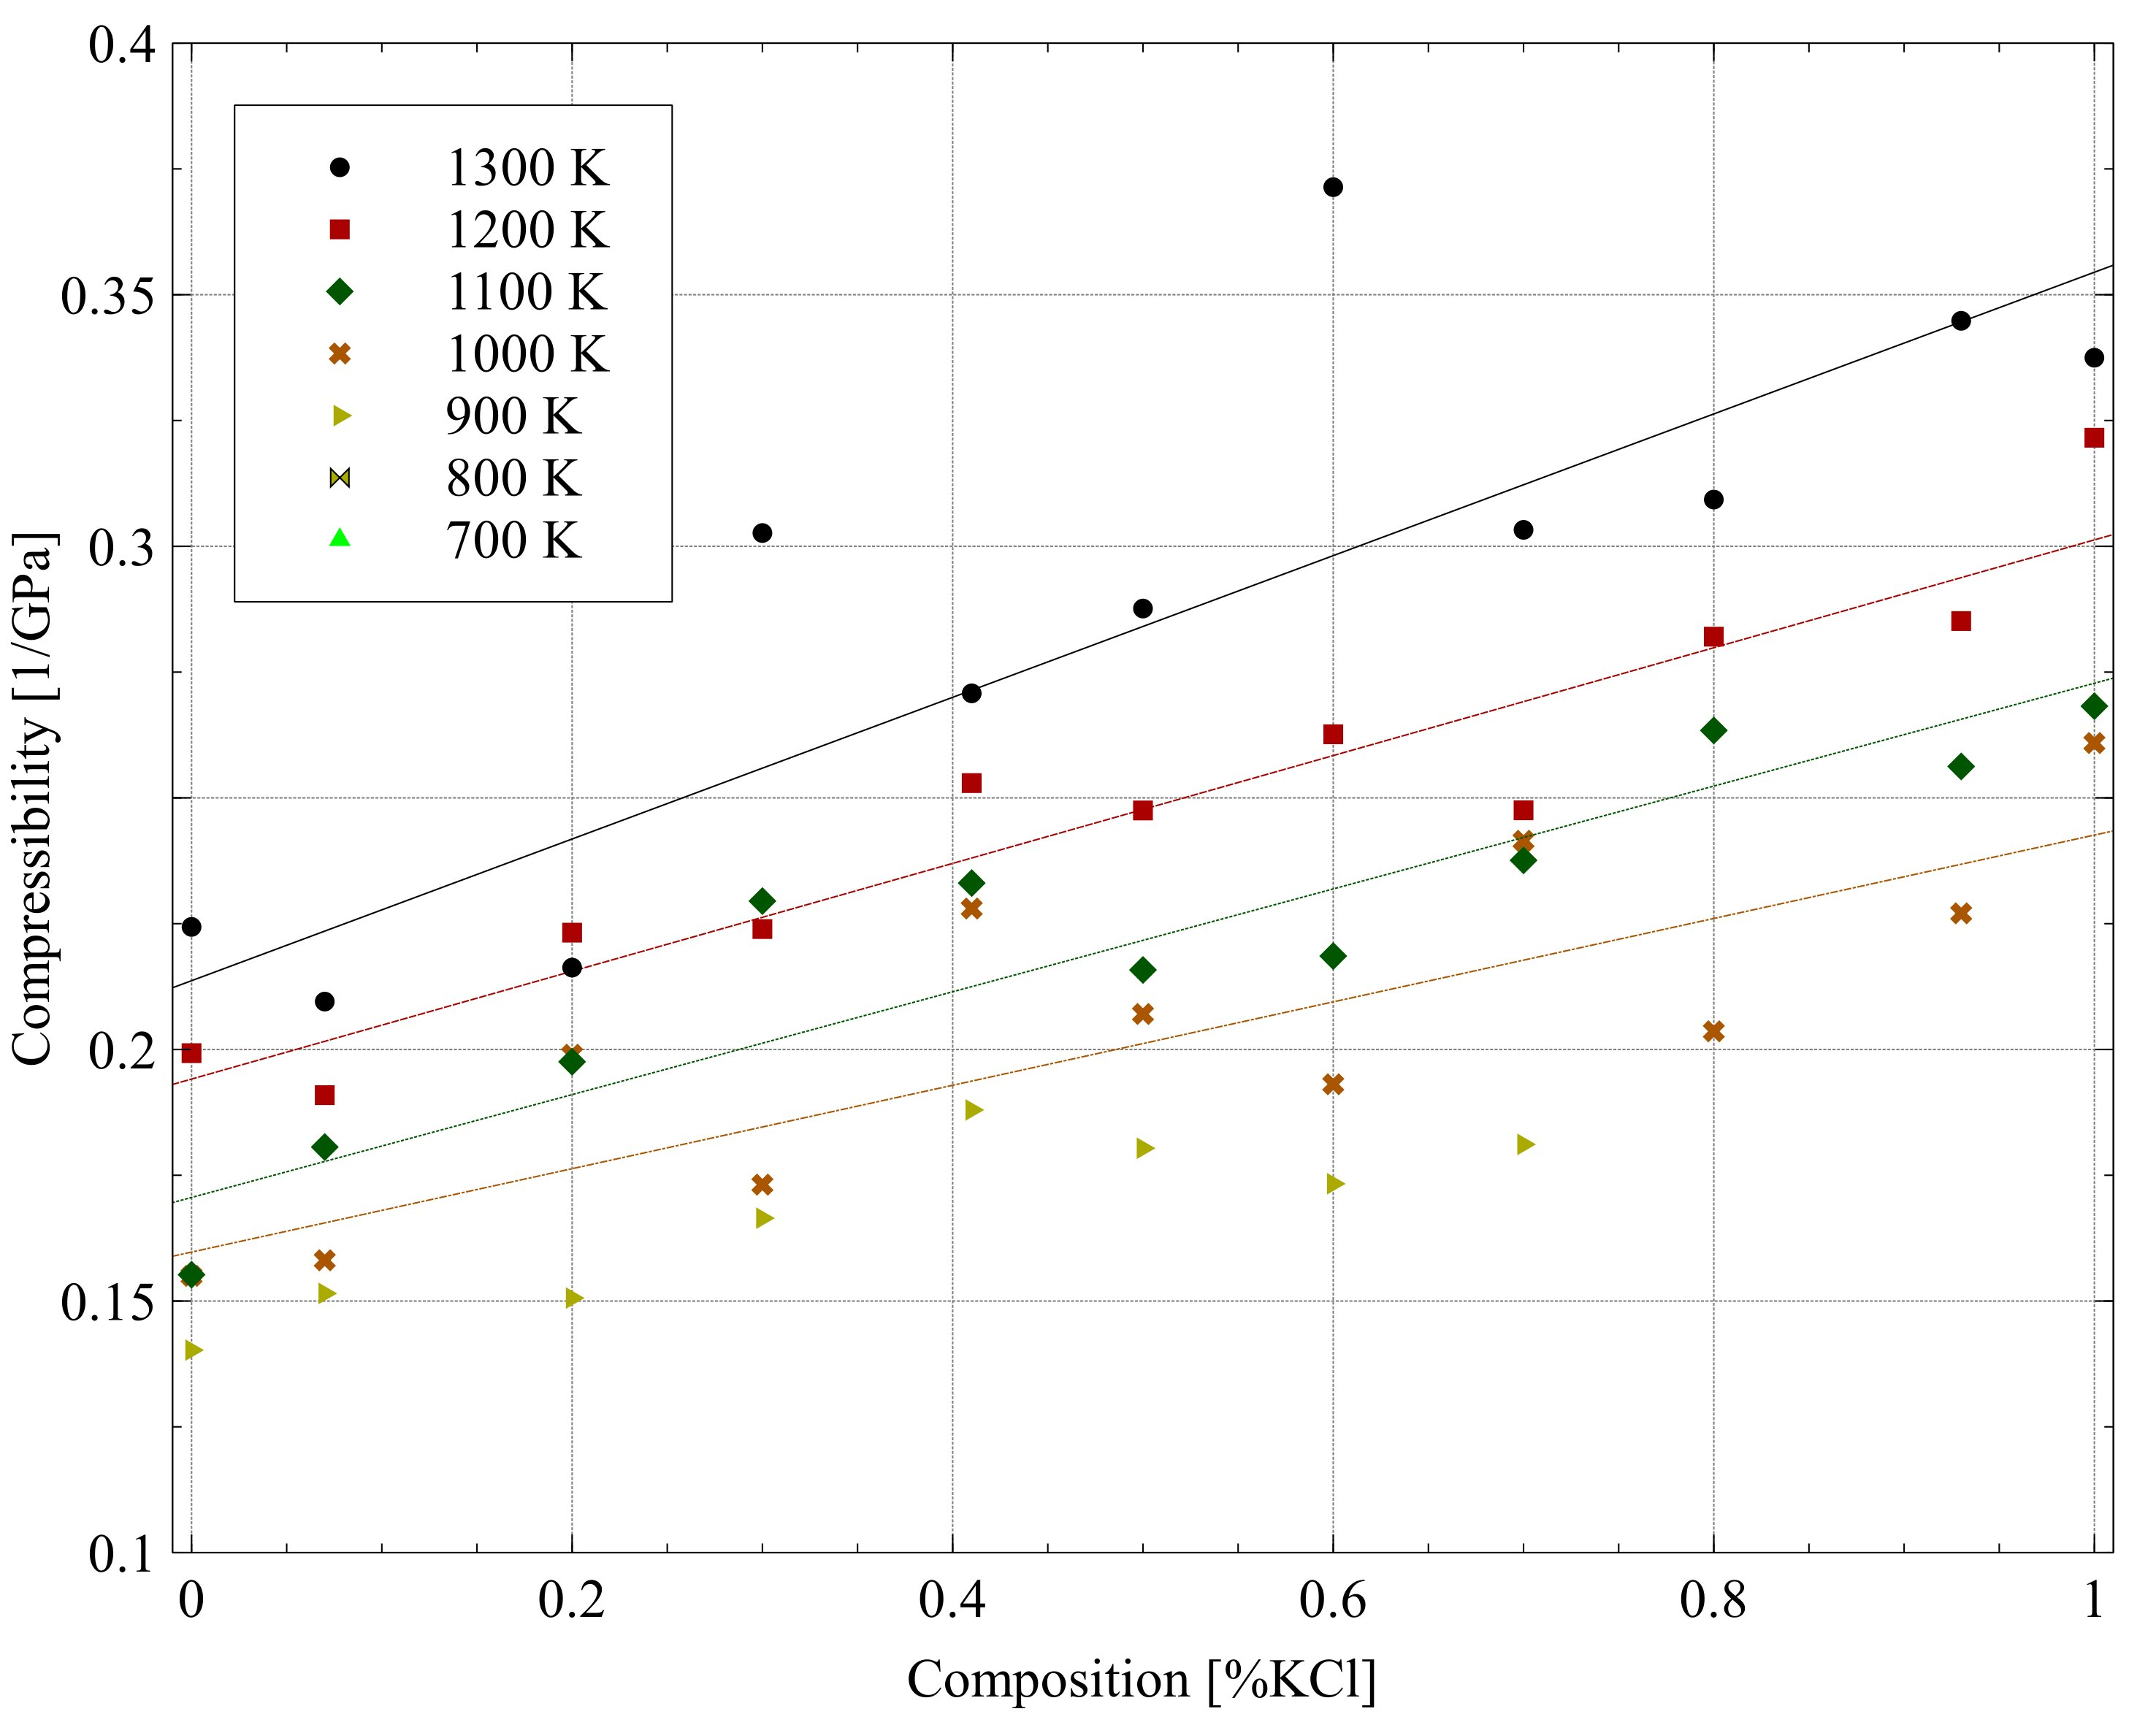
\includegraphics[width=0.8\textwidth]{images/compressibility.jpg} 
%DIFDELCMD <  %%%
\DIFdelendFL \DIFaddbeginFL 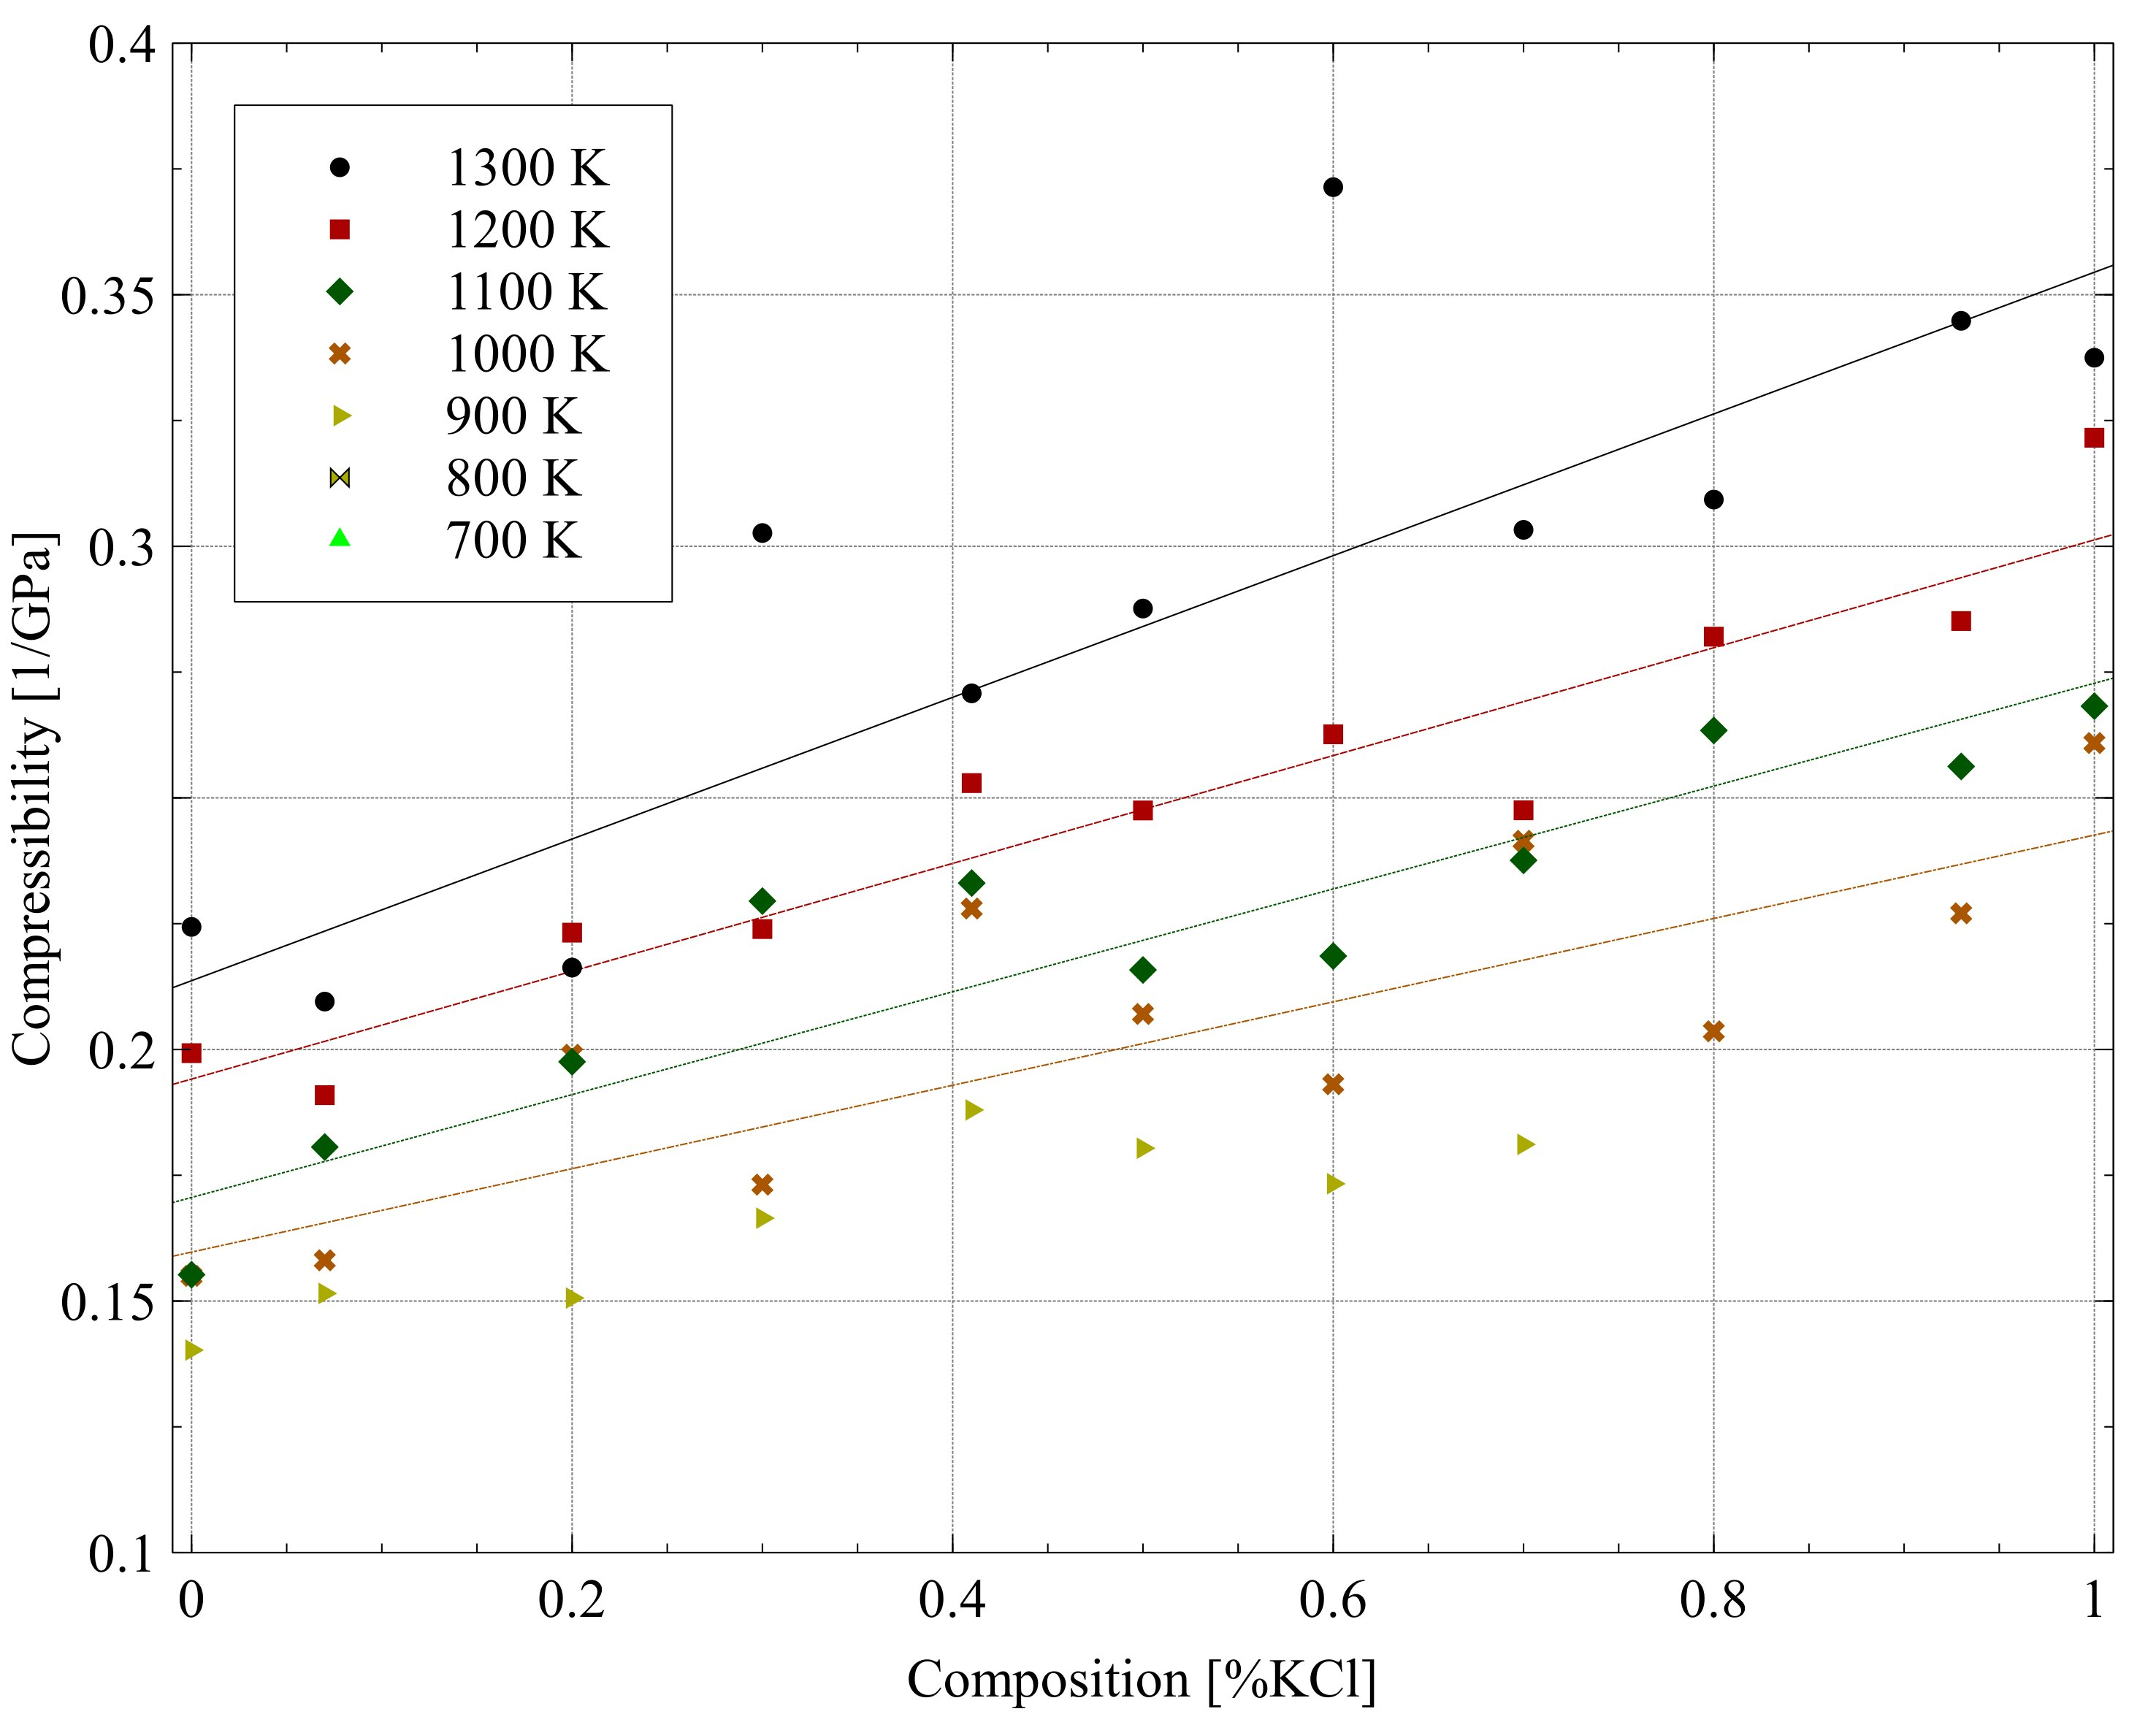
\includegraphics[width=0.7\textwidth]{images/compressibility.jpg} 
 \DIFaddendFL \caption{The compressibility of the LiCl-KCl system as a function of composition and temperature. Linear fits to each complete data set are shown as lines \DIFaddbeginFL \DIFaddFL{to better illustrate the trends in the data}\DIFaddendFL . }
 \label{fig:compressibility}
\end{figure} 

The heat capacity as a function of composition and temperature is shown in Fig. \ref{fig:cp}. \DIFaddbegin \DIFadd{The linear fits to the data at 1050 K and above are shown to illustrate overall trends of the data, not necessarily to suggest that a linear fit most appropriately suits the data. }\DIFaddend It can be observed that as the system becomes more KCl rich, the heat capacity tends to increase. Also, typically the smaller the temperature, the larger the heat capacity. It can be noted that the heat capacity values from AIMD are slightly under-predicting the experimental values of \DIFdelbegin \DIFdel{Janz \cite{Janz1974}, by 8.8}\DIFdelend \DIFaddbegin \DIFadd{Clark \cite{clark1973}, by 4.64}\DIFaddend \%. This is considered reasonable agreement.

\begin{figure}[h]
 \centering
 \DIFdelbeginFL %DIFDELCMD < 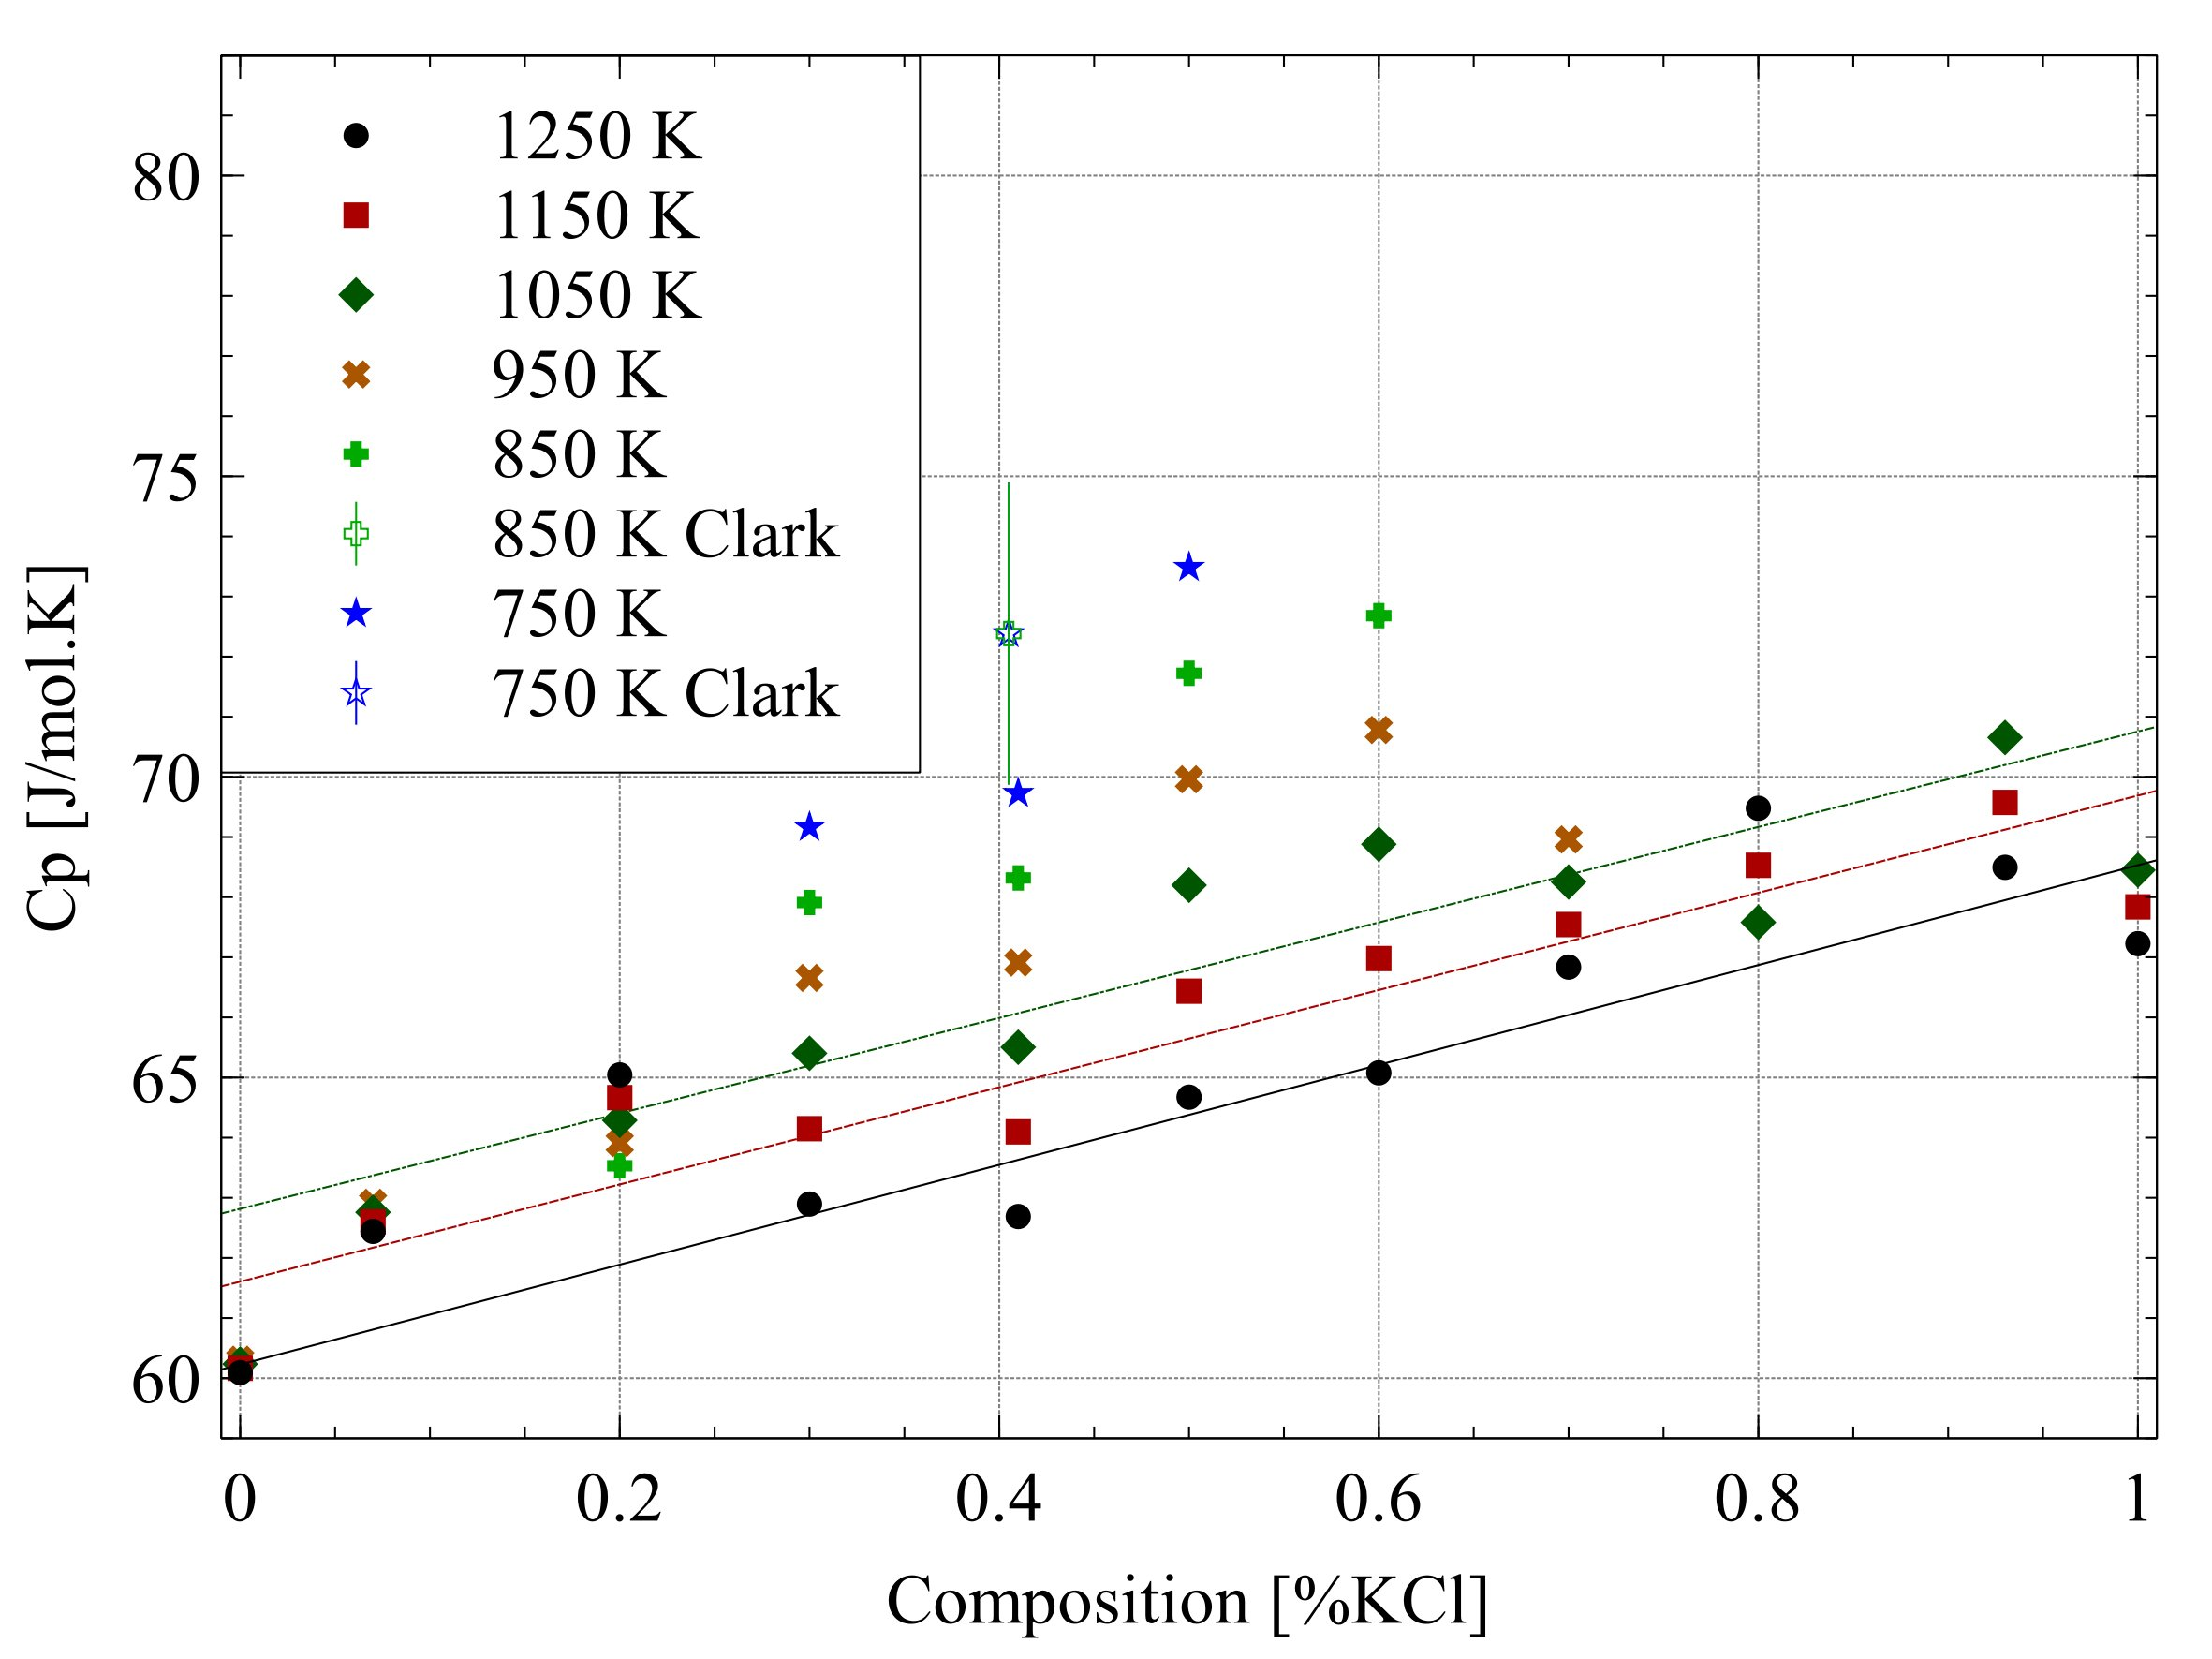
\includegraphics[width=0.8\textwidth]{images/cp.jpg} 
%DIFDELCMD <  %%%
\DIFdelendFL \DIFaddbeginFL 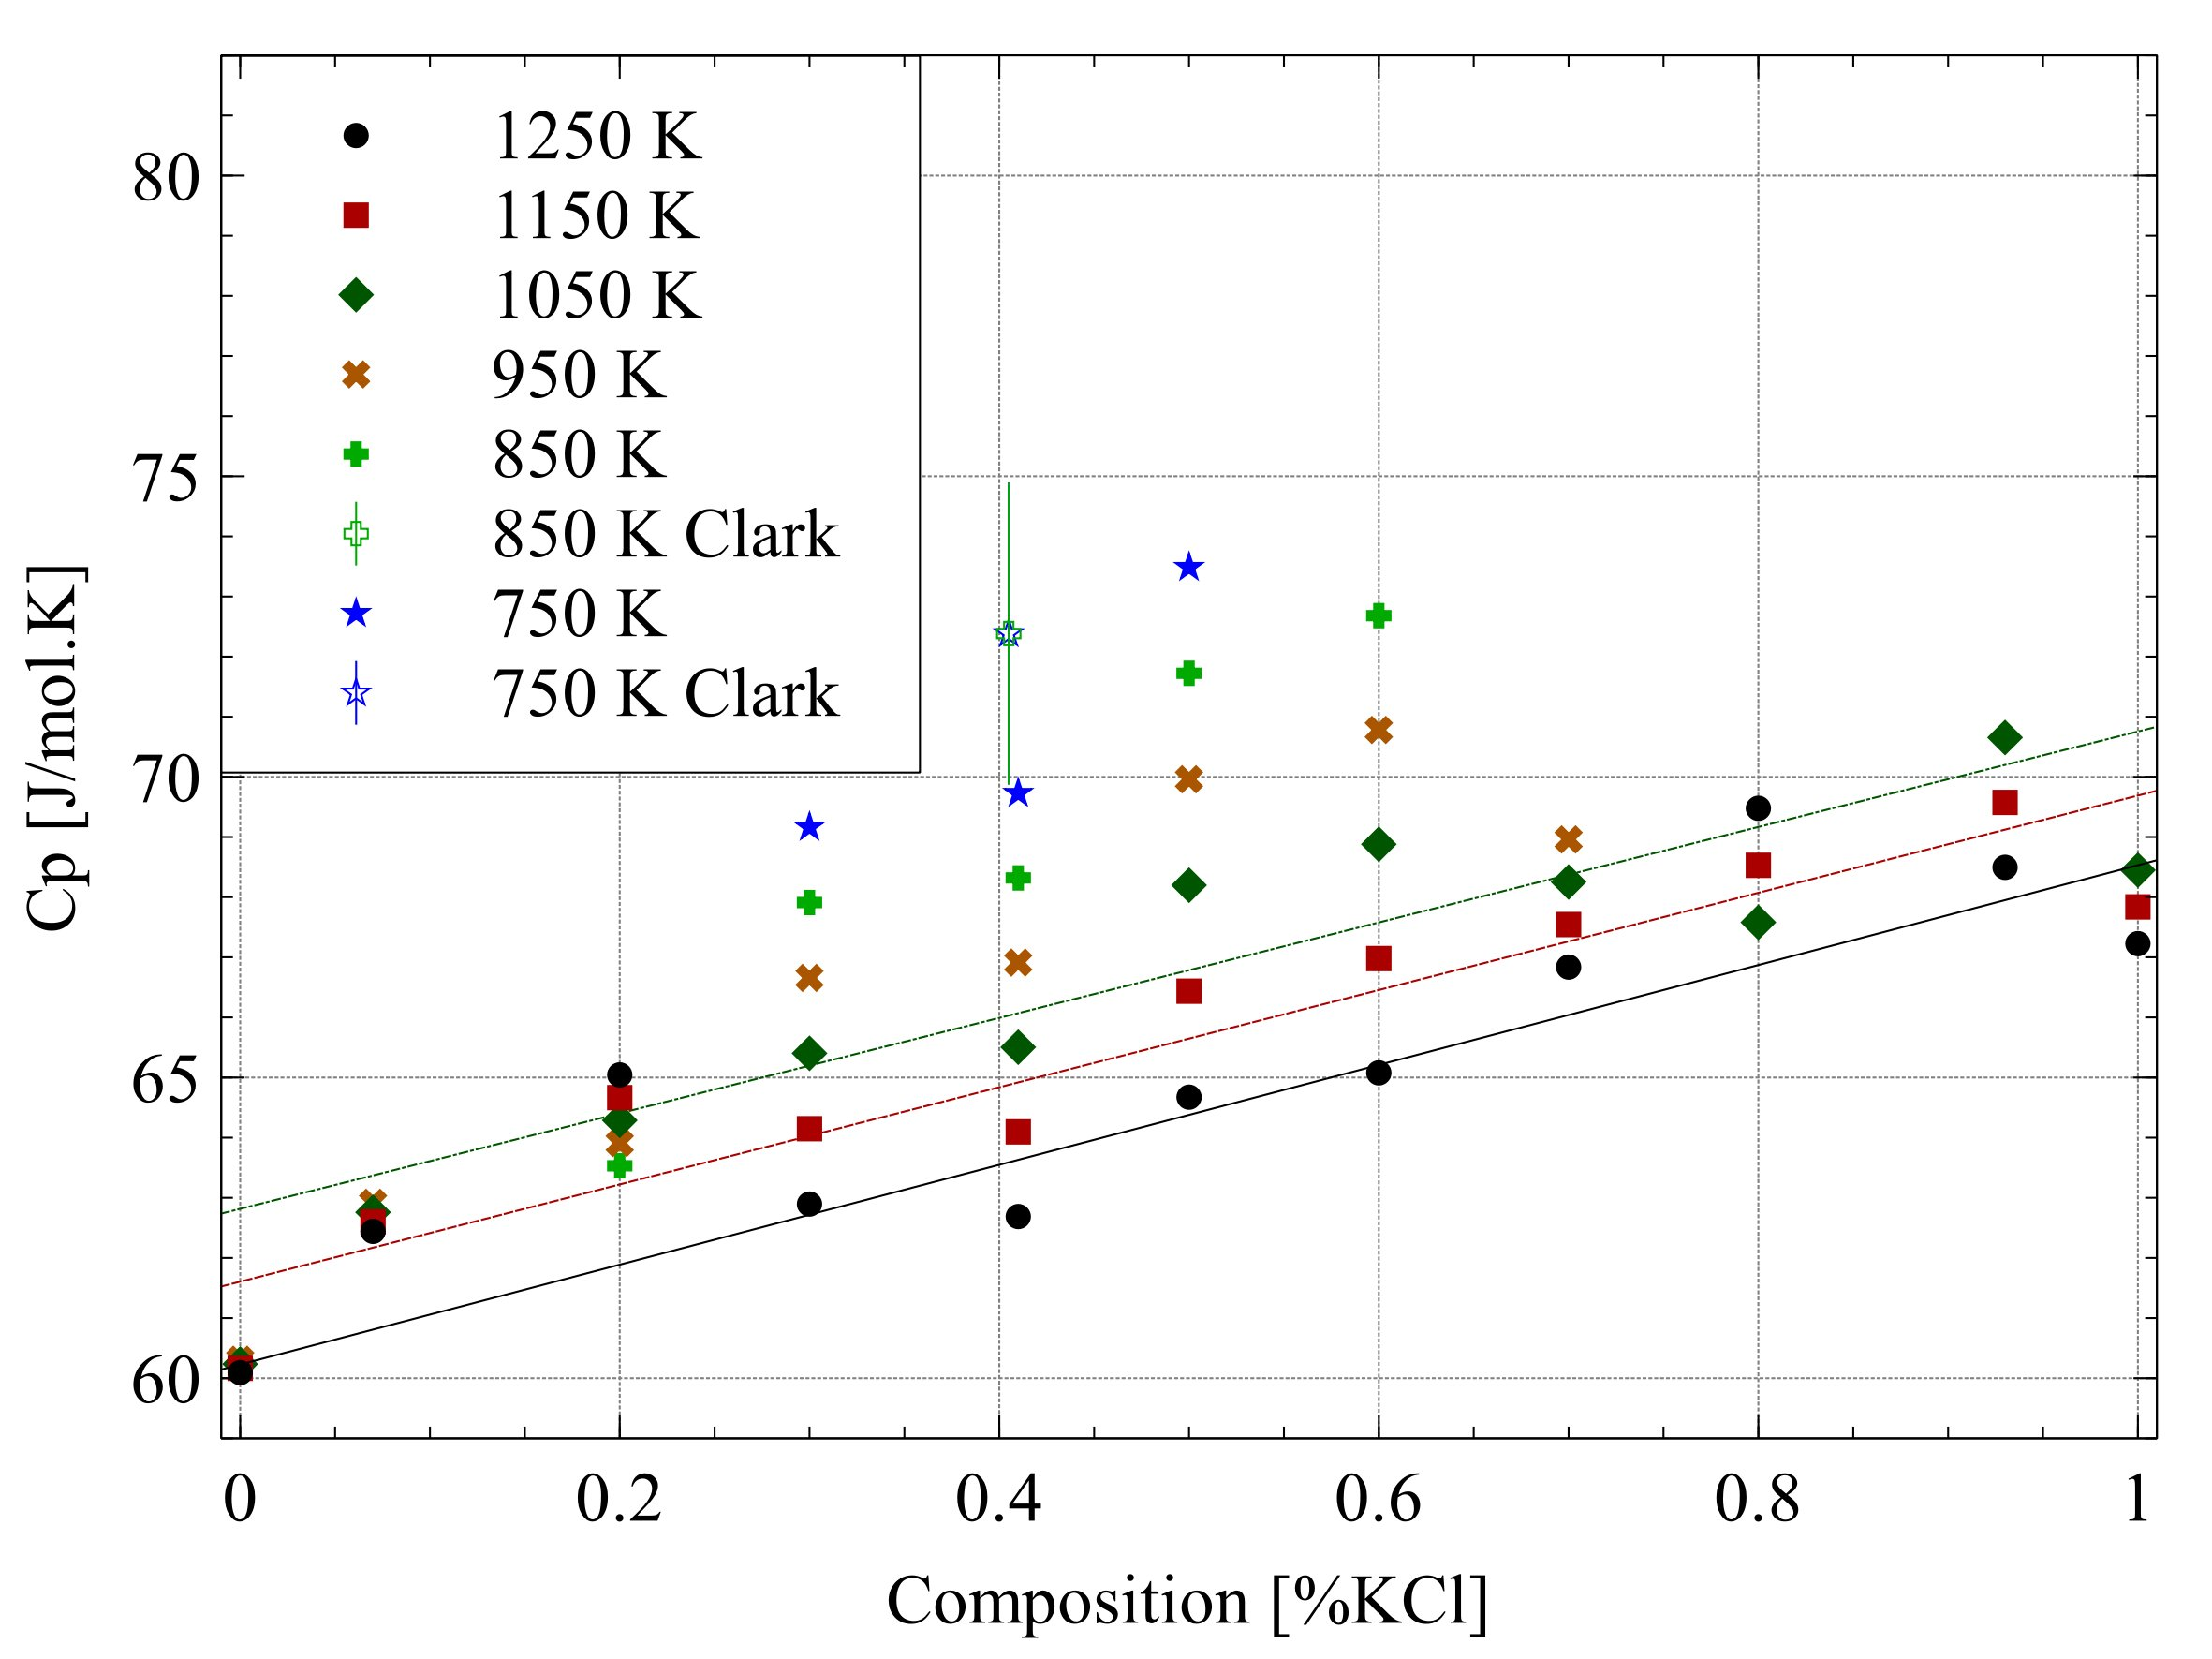
\includegraphics[width=0.7\textwidth]{images/cp.jpg} 
 \DIFaddendFL \caption{The heat capacity for the LiCl-KCl system as a function of composition. Literature from \DIFdelbeginFL \DIFdelFL{\cite{Janz1974}}\DIFdelendFL \DIFaddbeginFL \DIFaddFL{\cite{janz1975molten,clark1973}}\DIFaddendFL . Linear fits to each complete data set are shown as lines \DIFaddbeginFL \DIFaddFL{to better illustrate the trends in the data}\DIFaddendFL . }
 \label{fig:cp}   
\end{figure} 

\FloatBarrier

The enthalpy of mixing per molecule for the LiCl-KCl system can be seen below in Fig. \ref{fig:enthalpy}A, where negative values (lower formation energies) indicate the stability of the system. The most stable compound is the eutectic composition, which is to be expected. In Fig. \ref{fig:enthalpy}B there is a comparison to literature \cite{hersh1965enthalpies} at 1013 K, and the data matches the literature fairly well. It must be noted that the melting temperature of KCl is 1042 K \cite{Zhou2020}, while the computational data utilized in Fig. \ref{fig:enthalpy} is at 1000 K. It was determined that KCl is still a liquid at this point and can be used as a reference for liquid phase. \DIFaddbegin \DIFadd{This is due to the low level of subcooling and the short time period. The radial distribution function was analyzed to confirm the retention of a liquid structure. }\DIFaddend No lower temperatures \DIFdelbegin \DIFdel{could be }\DIFdelend \DIFaddbegin \DIFadd{were }\DIFaddend used due to the \DIFaddbegin \DIFadd{possibility of the }\DIFaddend onset of localized solidification.

\begin{figure}[h]
 \centering
 \DIFdelbeginFL %DIFDELCMD < 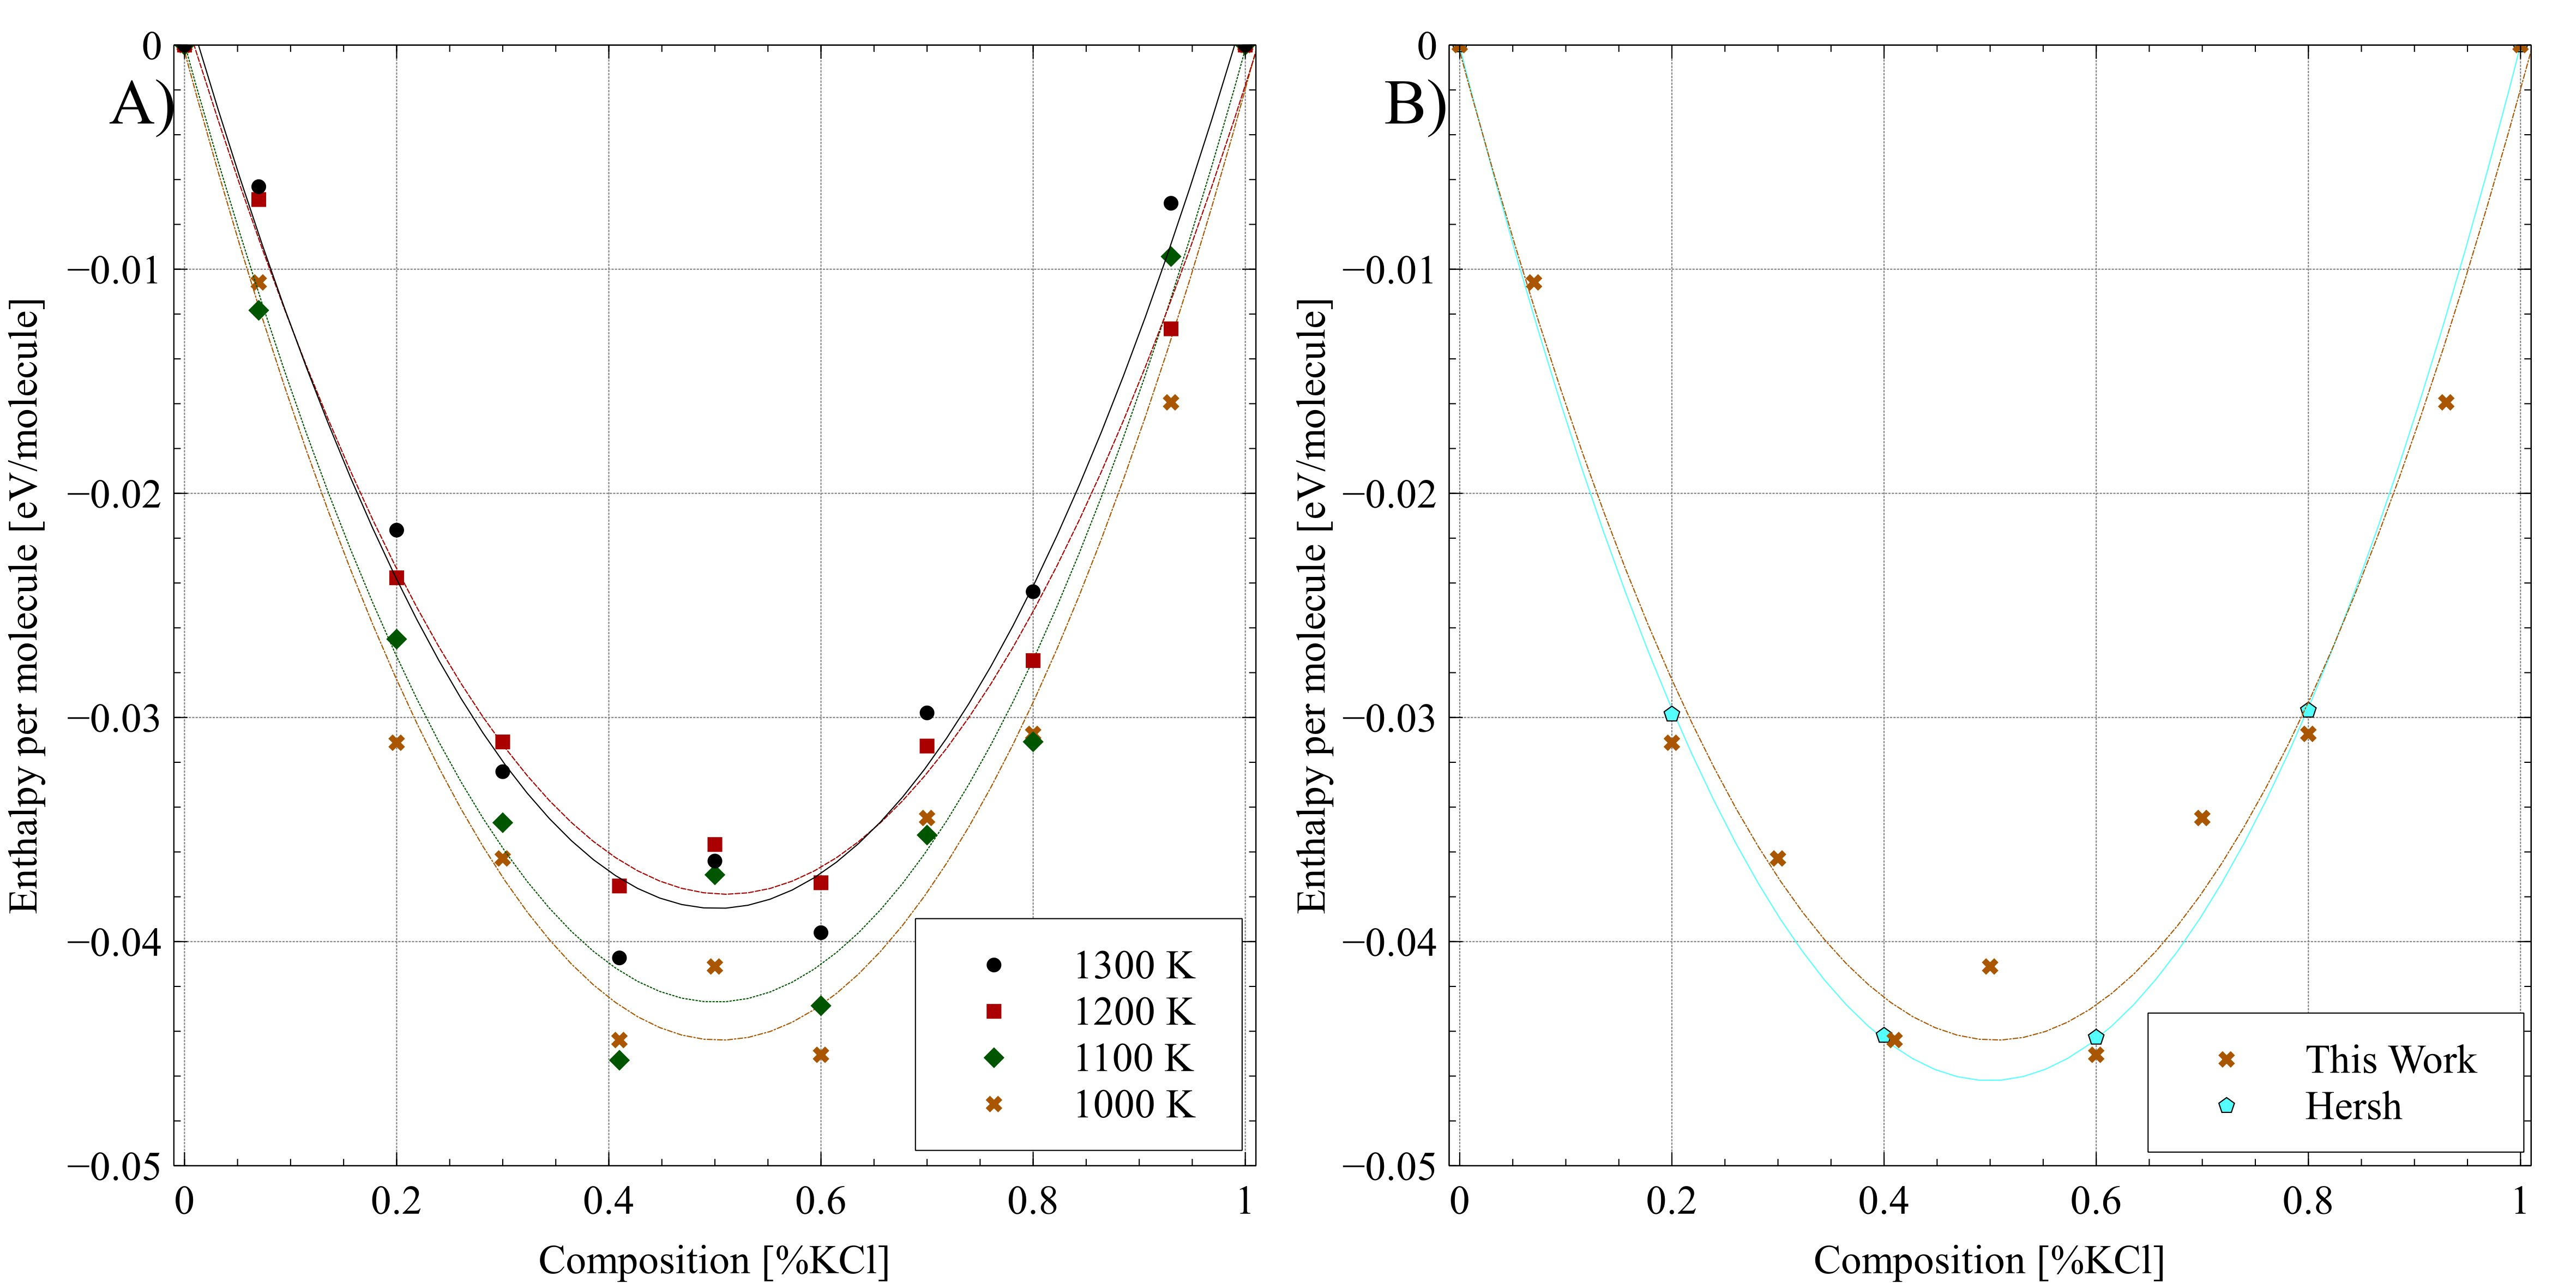
\includegraphics[width=0.8\textwidth]{images/enthalpy_combined.jpg} 
%DIFDELCMD <  %%%
\DIFdelendFL \DIFaddbeginFL 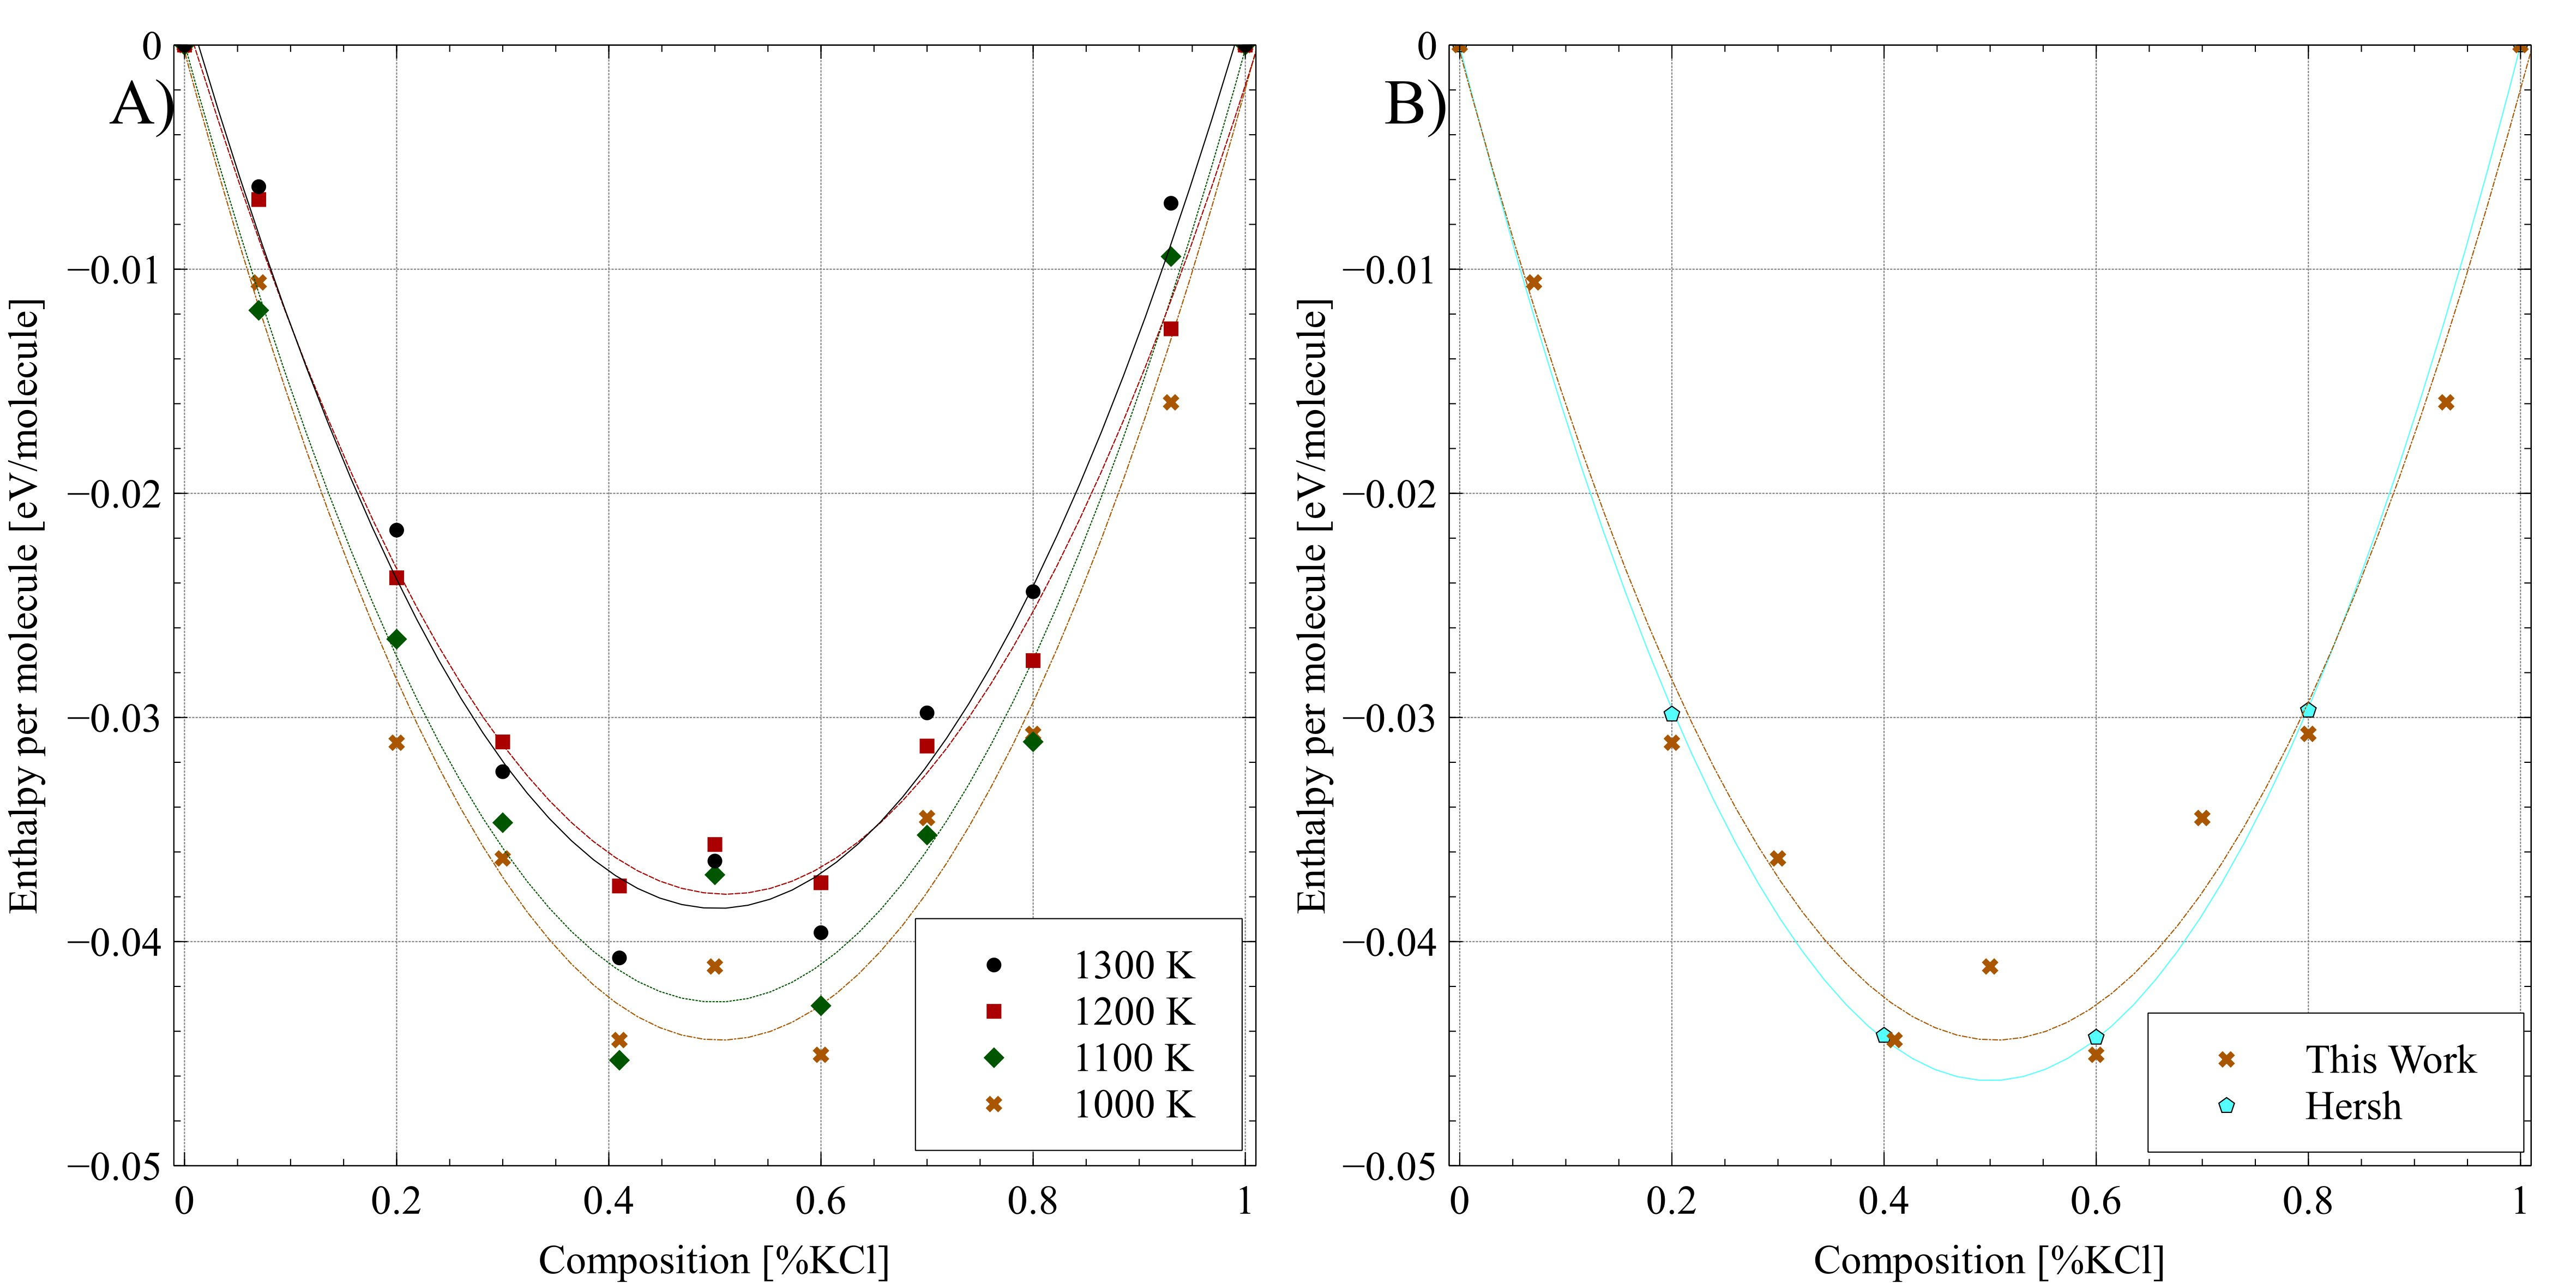
\includegraphics[width=1.0\textwidth]{images/enthalpy_combined.jpg} 
 \DIFaddendFL \caption{In A) the enthalpy of mixing per molecule of LiCl-KCl for the LiCl-KCl system. In B)  a comparison to Hersh \cite{hersh1965enthalpies} at 1013 K. Second order polynomial fits to each data set are shown as lines.}
 \label{fig:enthalpy}
\end{figure} 

The final property that was calculated is the Gibbs free energy of mixing of LiCl-KCl, shown in Fig. \ref{fig:gibb}A. It is again found that the minimum is around the eutectic composition, as would be expected. A comparison to the literature can be seen in Fig. \ref{fig:gibb}B, which shows the Gibbs free energy of mixing at 1173 K compared to AIMD by Nguyen et al. \cite{NGUYEN2021} and experimental data from the FTsalt-FACT database \cite{FTsalt} at 1173 K. What can be observed is that our AIMD simulation almost perfectly matches the experimental data across the compositional spectrum.

\begin{figure}[h]
 \centering
 \DIFdelbeginFL %DIFDELCMD < 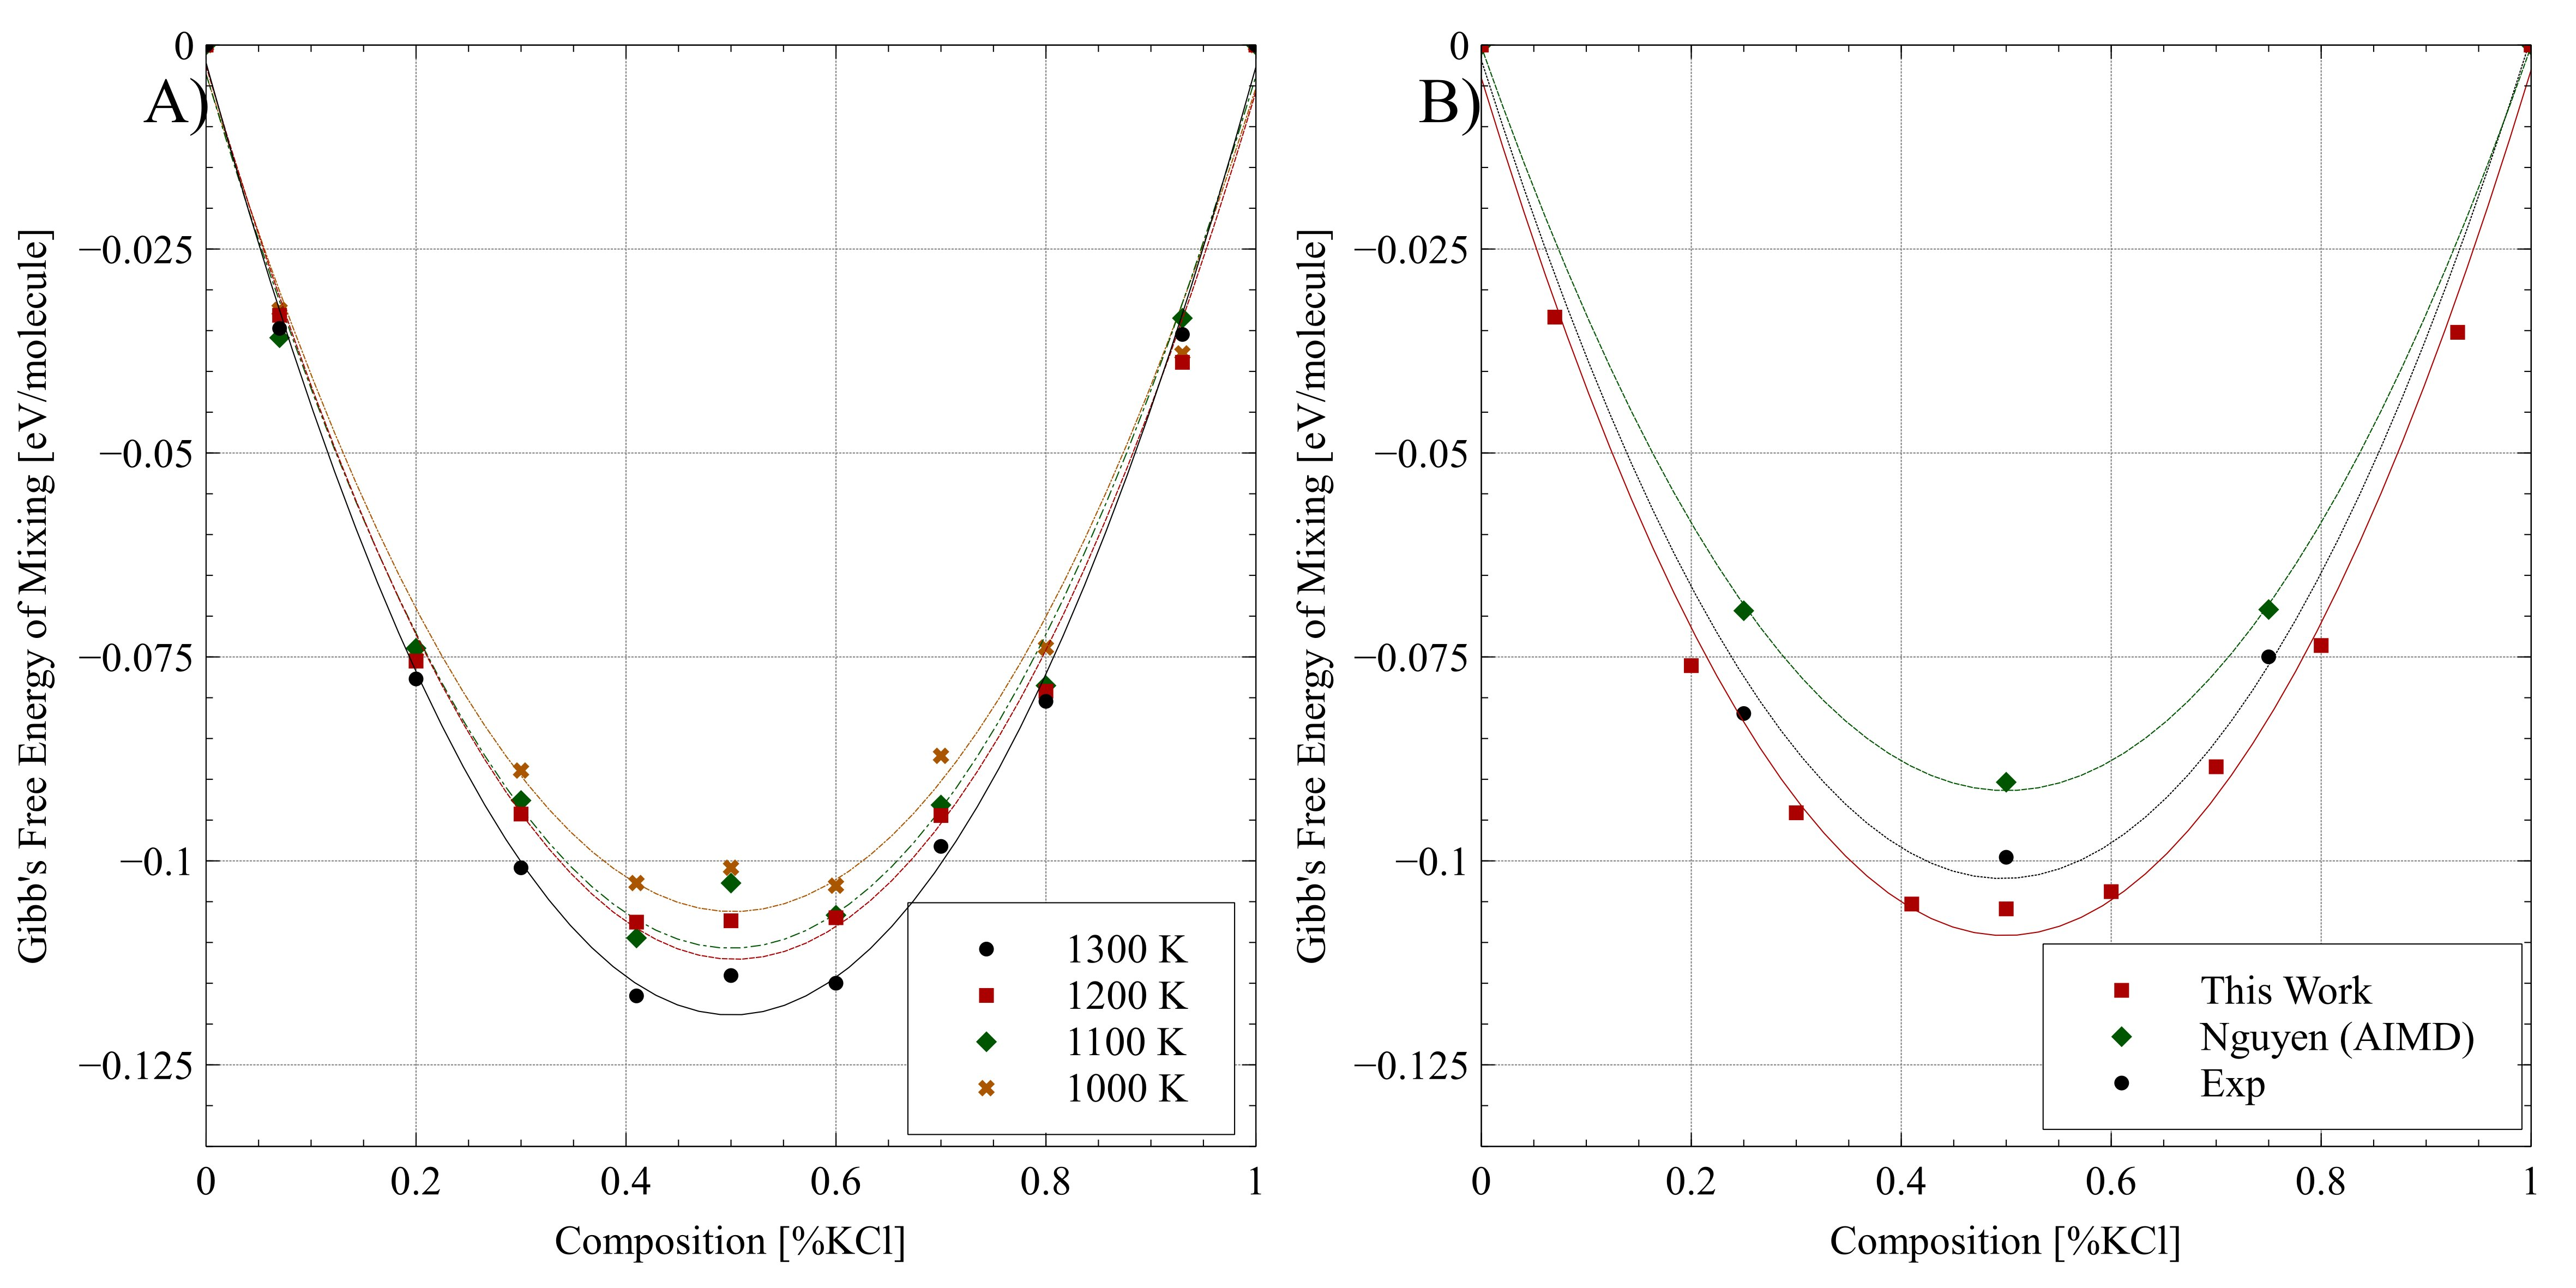
\includegraphics[width=0.8\textwidth]{images/gibbs_mixxing_combined.jpg} 
%DIFDELCMD <  %%%
\DIFdelendFL \DIFaddbeginFL 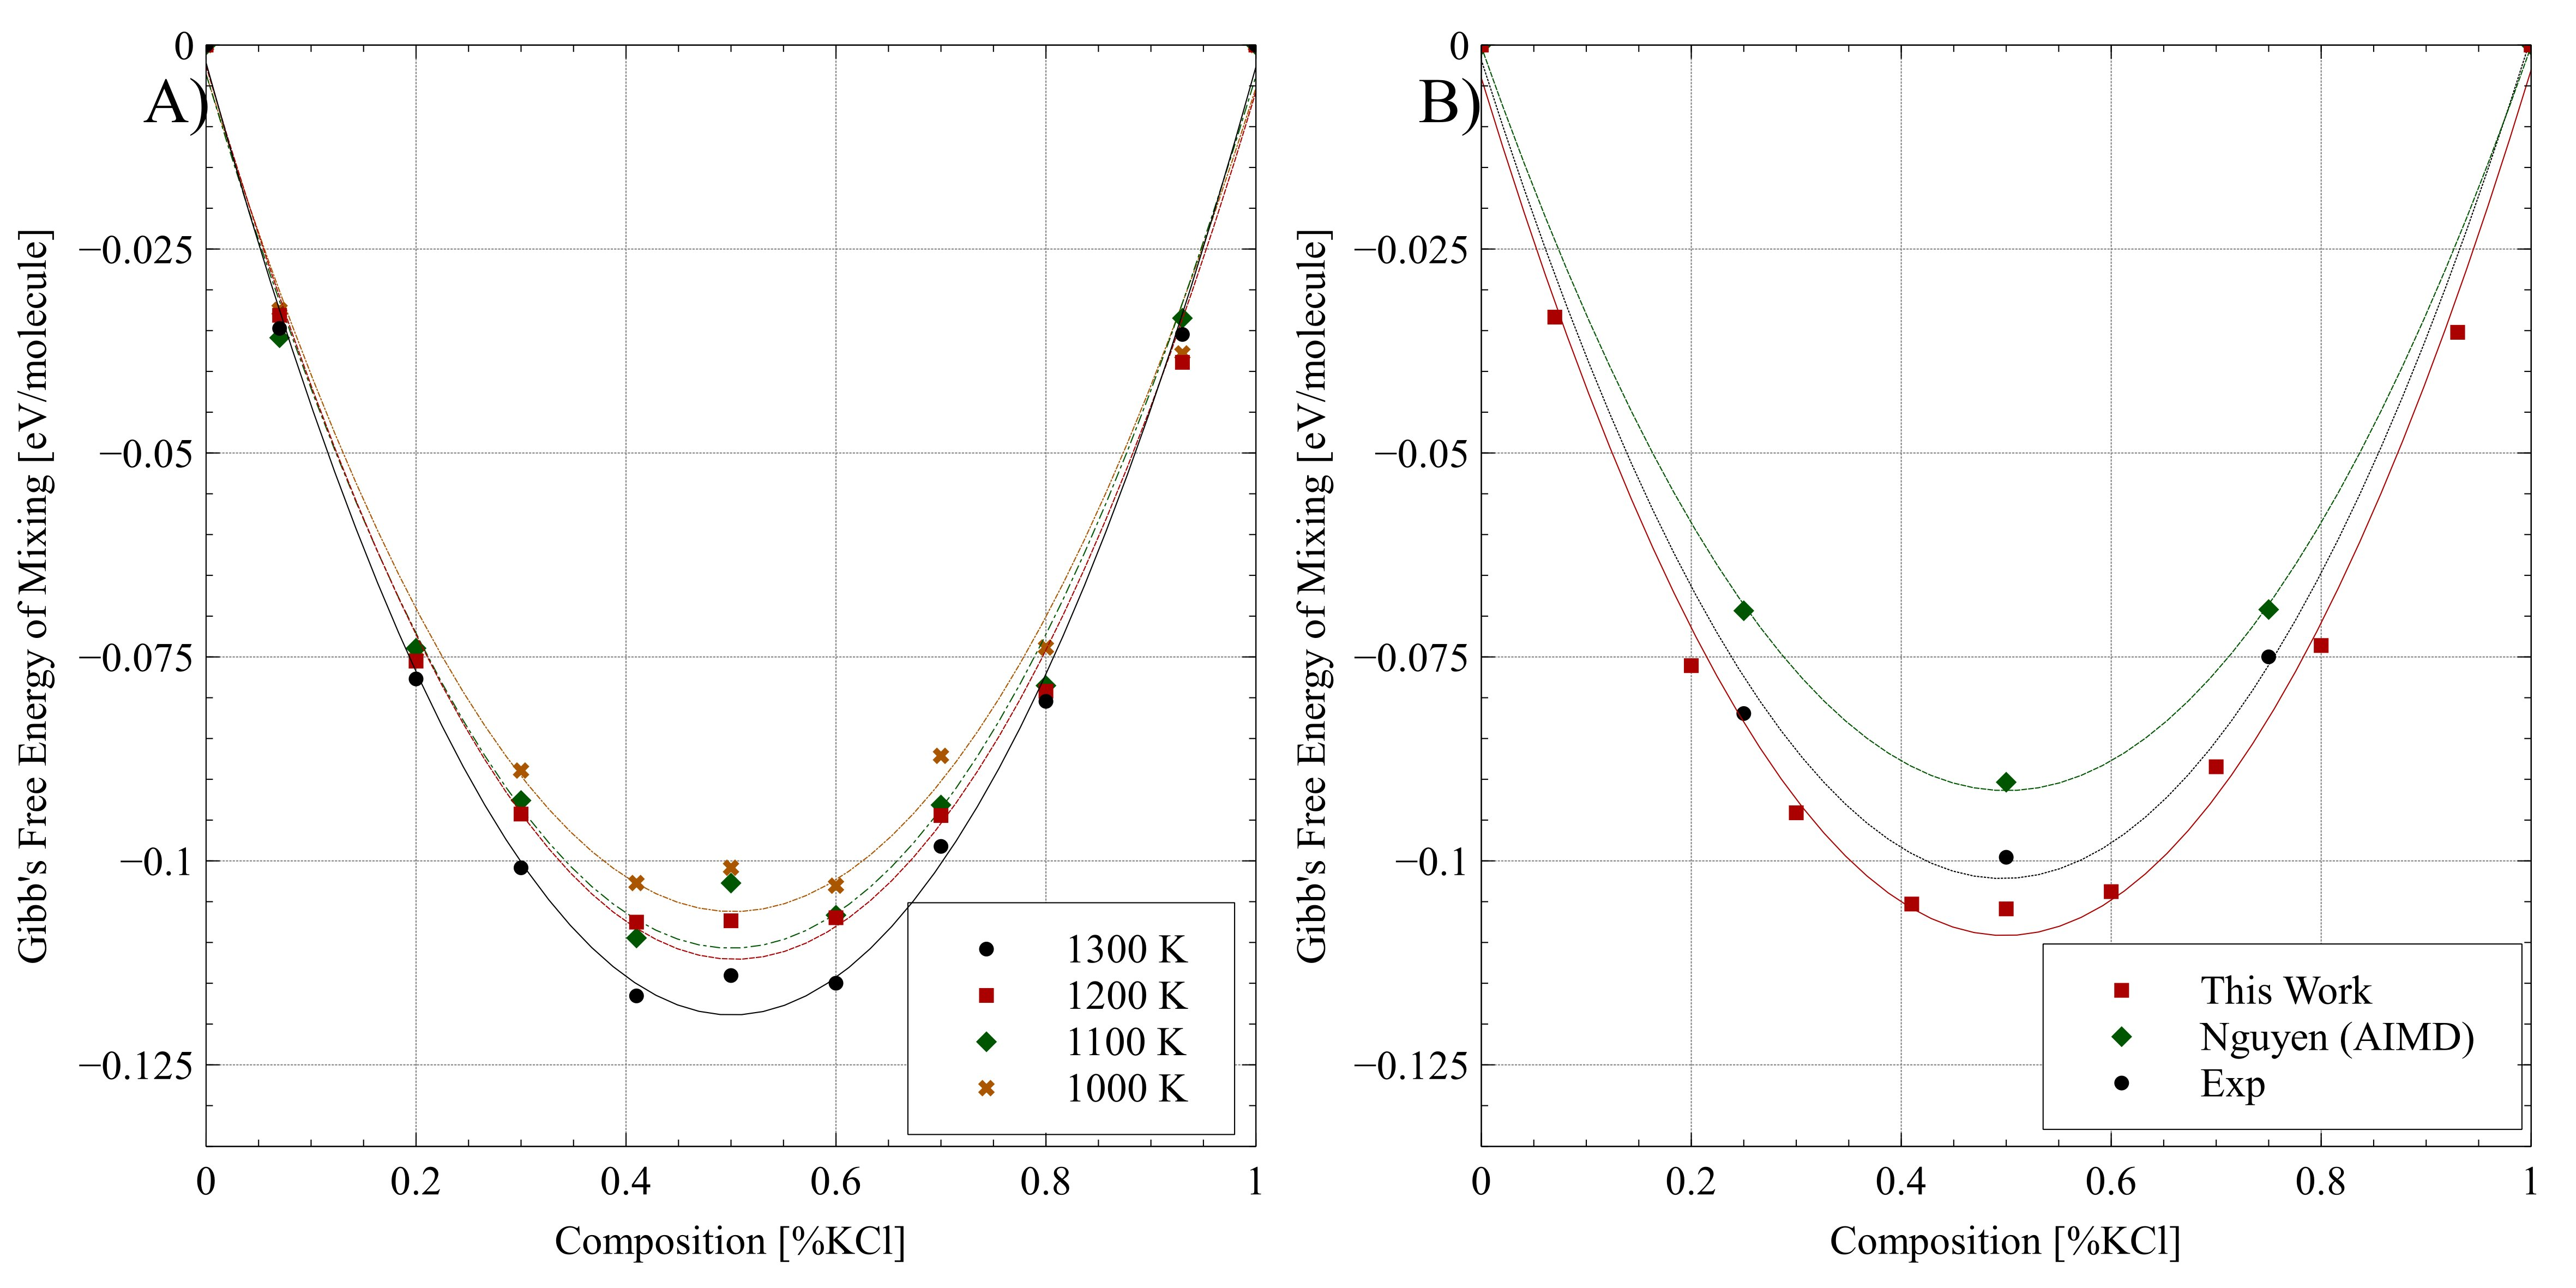
\includegraphics[width=1.0\textwidth]{images/gibbs_mixxing_combined.jpg} 
 \DIFaddendFL \caption{In A) the Gibb's free energy of mixing for the LiCl-KCl system. In B) a comparsion to literature at 1173K can be seen with AIMD from Nguyen \cite{NGUYEN2021} and experimental data from FTsalt-FACT data base \cite{FTsalt}. Second order polynomial fits to each data set are shown as lines.}
 \label{fig:gibb}
\end{figure} 

\FloatBarrier

\subsection{Experimental Results}

\DIFaddbegin \subsubsection{\DIFadd{Density Measurements}}

\DIFaddend Experimental values of the density of LiCl-KCl compositions in the liquid state are shown in Fig. \ref{fig:density_exp} with temperature-dependent equations given in Table \ref{table1}. All compositions of LiCl-KCl show a linear relationship between density and temperature. The decrease in density with increasing temperature becomes slightly greater with increasing concentration of KCl. The experimental error was computed \DIFaddbegin \DIFadd{based upon propagation of the errors of the measurements of the mass, buoyant weight, reference volume, coefficient of thermal expansion, and temperature. The error was computed }\DIFaddend to be approximately 0.7\% for all calculated densities, with the temperature measurement uncertainty being between 2.5 and 3.6 K. 

\begin{figure}[h]
 \centering
 \DIFdelbeginFL %DIFDELCMD < 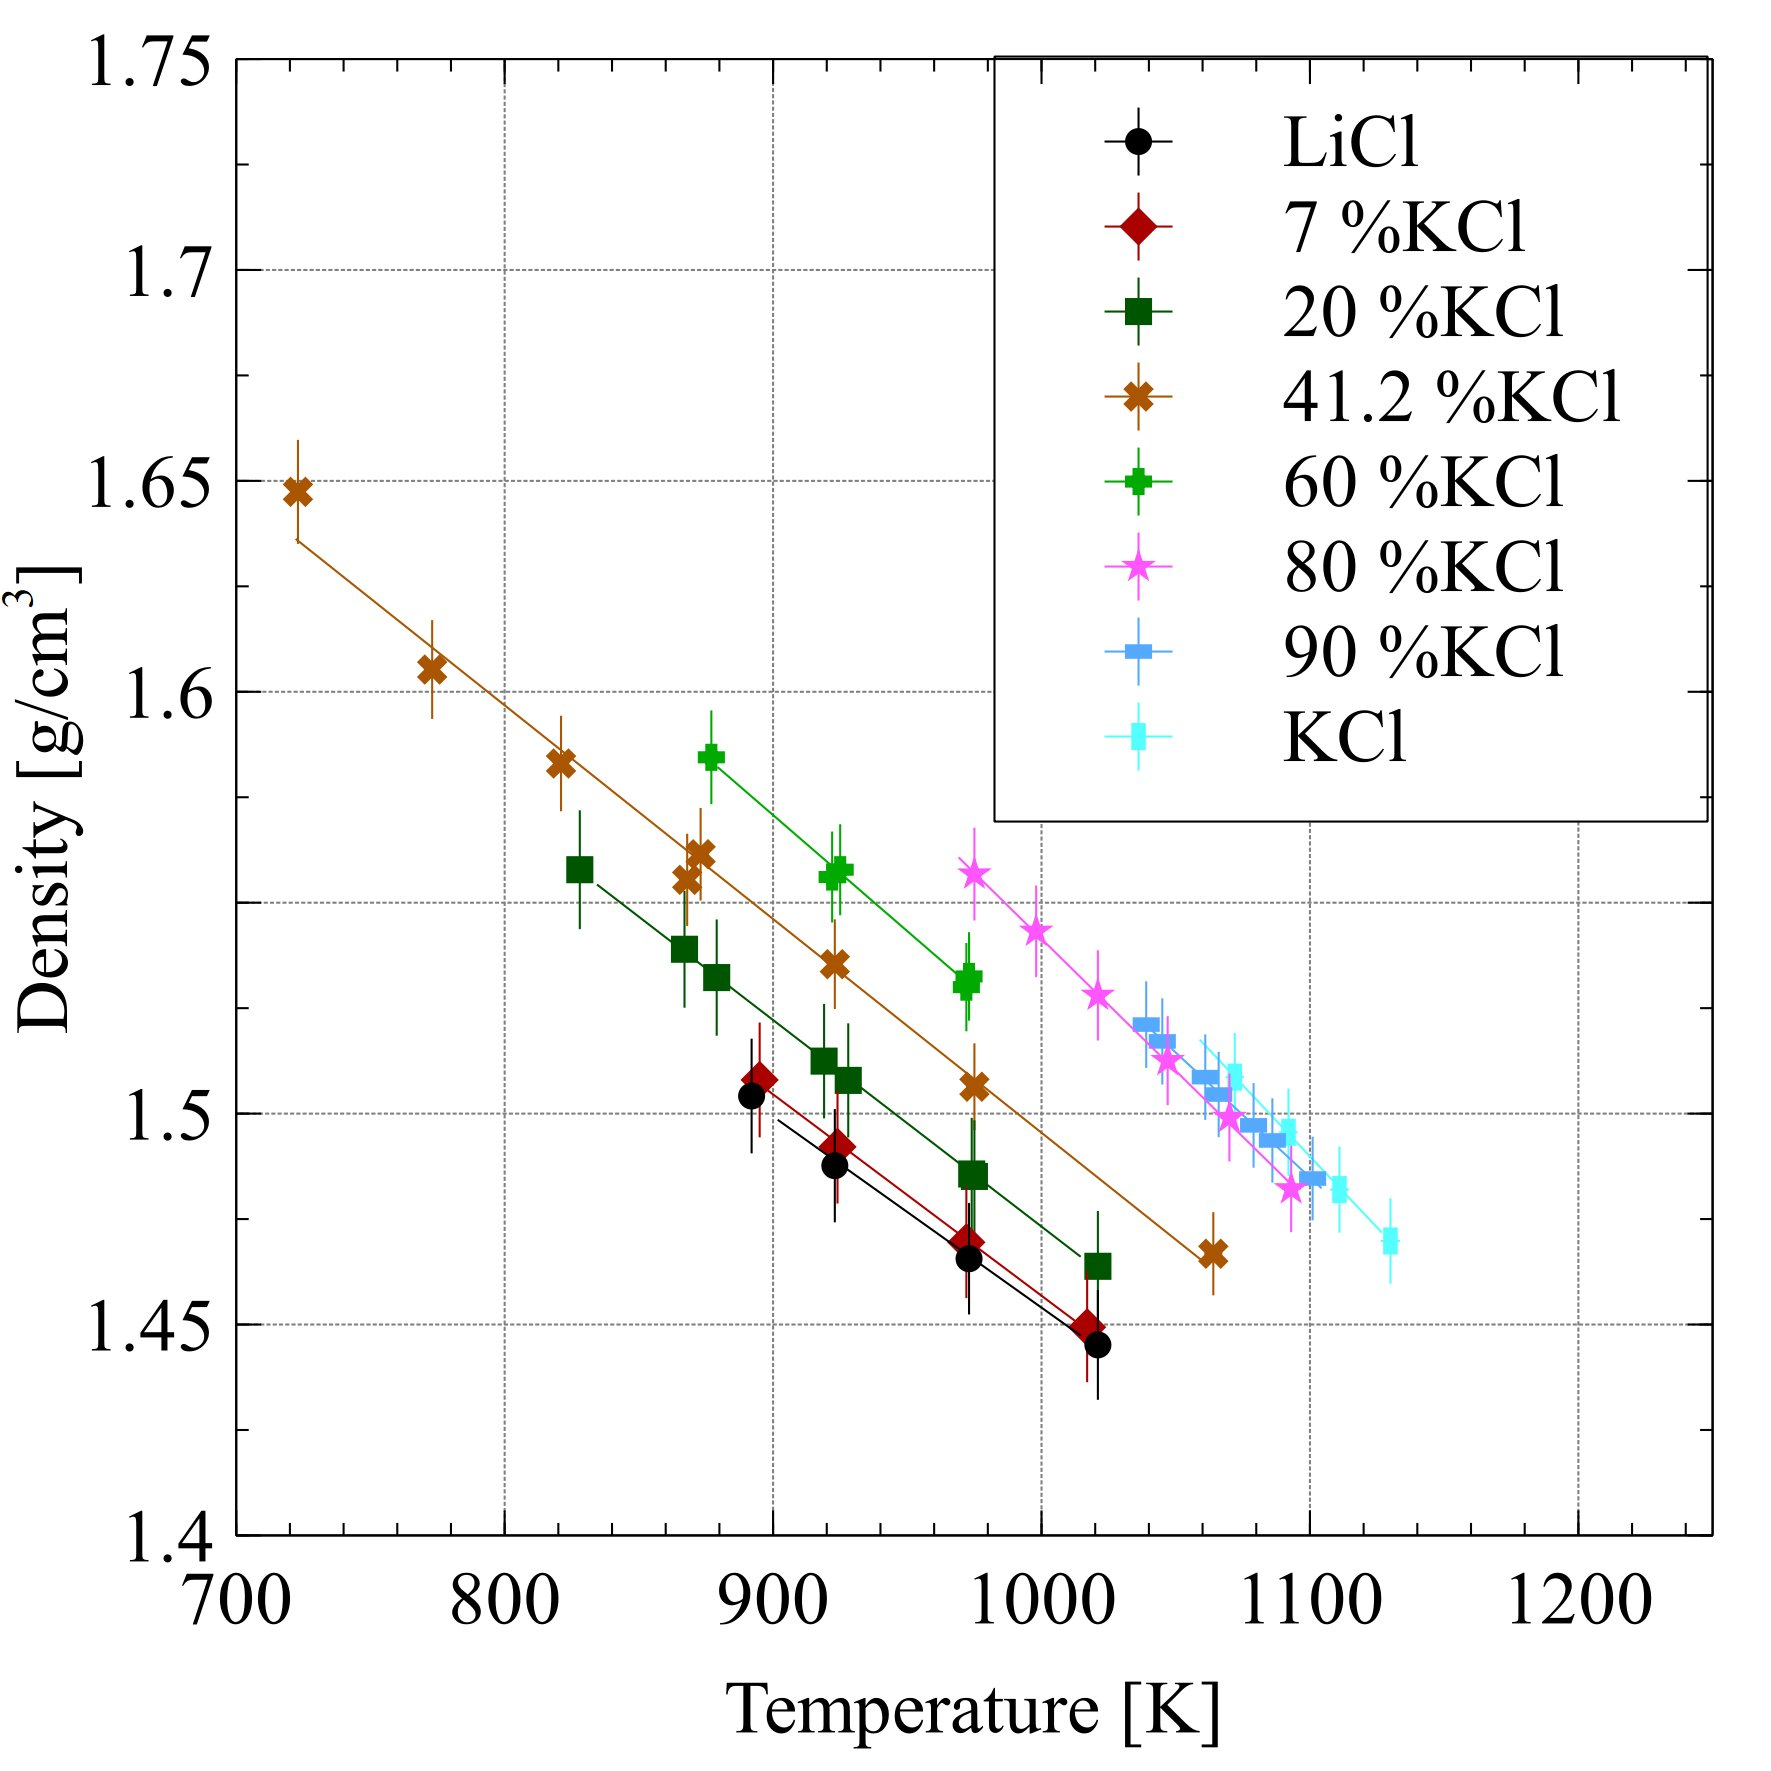
\includegraphics[width=0.8\textwidth]{images/density_exp.jpg} 
%DIFDELCMD <  %%%
\DIFdelendFL \DIFaddbeginFL 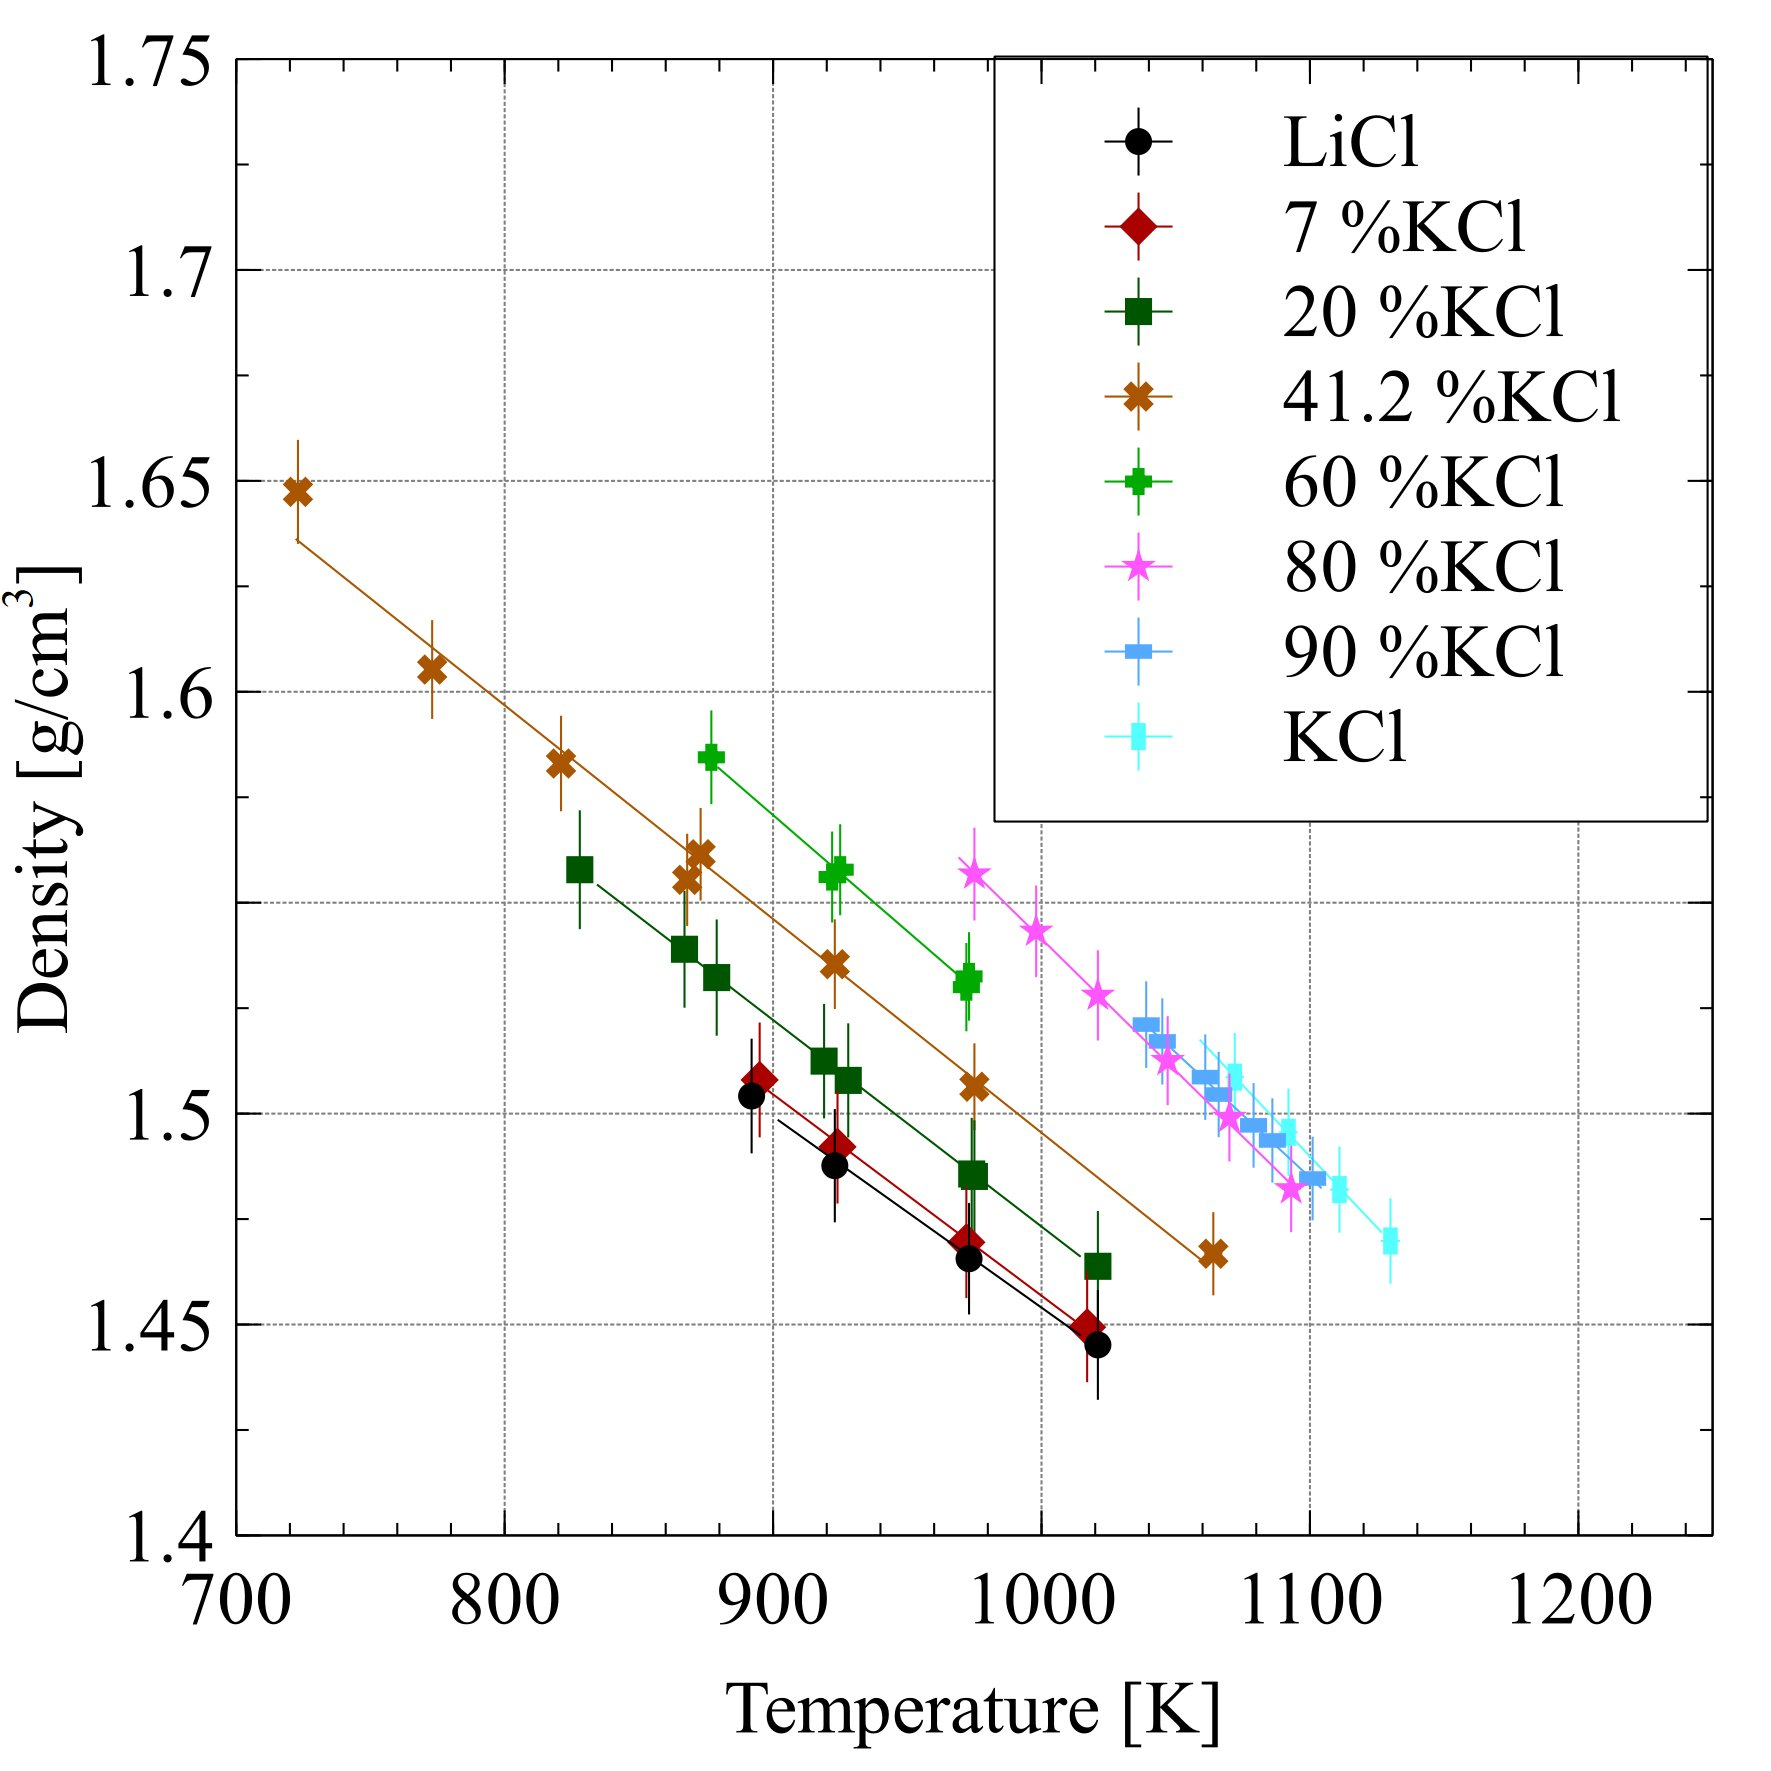
\includegraphics[width=0.7\textwidth]{images/density_exp.jpg} 
 \DIFaddendFL \caption{Experimental density values of LiCl-KCl mixtures.}
 \label{fig:density_exp}
\end{figure} 

\DIFdelbegin %DIFDELCMD < \begin{table}[]
%DIFDELCMD < %%%
\DIFdelendFL \DIFaddbeginFL \begin{table}[h]
\DIFaddendFL \centering
\caption{Experimental temperature-dependent equations of density for various compositions of LiCl-KCl}
\DIFdelbeginFL %DIFDELCMD < \begin{tabular}{|c|c|c|}
%DIFDELCMD < %%%
\DIFdelendFL
\begin{tabular}{|c|c|c|c|}
\hline
\multicolumn{4}{|c|}{$\rho$ = $\alpha$ + $\beta$ T}\\
\hline
mol\% KCl & $\alpha$ (g cm$^{-3}$) & $\beta$ (g cm$^{-3}$ K$^{-1}$) \DIFaddbeginFL & \DIFaddFL{r$^{2}$}\DIFaddendFL \\
\hline
100       & \DIFdelbeginFL \DIFdelFL{2.2315         }\DIFdelendFL \DIFaddbeginFL \DIFaddFL{2.235         }\DIFaddendFL & \DIFdelbeginFL \DIFdelFL{-0.000674         }\DIFdelendFL \DIFaddbeginFL \DIFaddFL{-0.000676        }& \DIFaddFL{0.996 }\DIFaddendFL \\
90        & \DIFdelbeginFL \DIFdelFL{2.1296         }\DIFdelendFL \DIFaddbeginFL \DIFaddFL{2.133         }\DIFaddendFL & \DIFdelbeginFL \DIFdelFL{-0.000586         }\DIFdelendFL \DIFaddbeginFL \DIFaddFL{-0.000588        }& \DIFaddFL{0.999 }\DIFaddendFL \\
80        & \DIFdelbeginFL \DIFdelFL{2.1677         }\DIFdelendFL \DIFaddbeginFL \DIFaddFL{2.171         }\DIFaddendFL & \DIFdelbeginFL \DIFdelFL{-0.000626         }\DIFdelendFL \DIFaddbeginFL \DIFaddFL{-0.000628        }& \DIFaddFL{0.999 }\DIFaddendFL \\
60        & \DIFdelbeginFL \DIFdelFL{2.0663         }\DIFdelendFL \DIFaddbeginFL \DIFaddFL{2.070         }\DIFaddendFL & \DIFdelbeginFL \DIFdelFL{-0.000550         }\DIFdelendFL \DIFaddbeginFL \DIFaddFL{-0.000514        }& \DIFaddFL{0.993 }\DIFaddendFL \\
41.8      & \DIFdelbeginFL \DIFdelFL{2.0060         }\DIFdelendFL \DIFaddbeginFL \DIFaddFL{2.010         }\DIFaddendFL & \DIFdelbeginFL \DIFdelFL{-0.000510         }\DIFdelendFL \DIFaddbeginFL \DIFaddFL{-0.000512        }& \DIFaddFL{0.990 }\DIFaddendFL \\
20        & \DIFdelbeginFL \DIFdelFL{1.9627         }\DIFdelendFL \DIFaddbeginFL \DIFaddFL{1.966         }\DIFaddendFL & \DIFdelbeginFL \DIFdelFL{-0.000489         }\DIFdelendFL \DIFaddbeginFL \DIFaddFL{-0.000490        }& \DIFaddFL{1.000 }\DIFaddendFL \\
7         & \DIFdelbeginFL \DIFdelFL{1.9356         }\DIFdelendFL \DIFaddbeginFL \DIFaddFL{1.939         }\DIFaddendFL & \DIFdelbeginFL \DIFdelFL{-0.000478         }\DIFdelendFL \DIFaddbeginFL \DIFaddFL{-0.000479        }& \DIFaddFL{0.999 }\DIFaddendFL \\
0         & \DIFdelbeginFL \DIFdelFL{1.9086         }\DIFdelendFL \DIFaddbeginFL \DIFaddFL{1.912         }\DIFaddendFL & \DIFdelbeginFL \DIFdelFL{-0.000454         }\DIFdelendFL \DIFaddbeginFL \DIFaddFL{-0.000455        }& \DIFaddFL{0.998 }\DIFaddendFL \\
\hline
\end{tabular}
\label{table1}
\end{table}

\FloatBarrier

\DIFaddbegin \subsubsection{\DIFadd{Transition Temperature Measurements}}

\DIFadd{The eutectic and melting temperatures for each heating rate were determined by averaging the onset (eutectic temperature) and end point (melting temperature) from three heating cycles. The reported eutectic and melting point temperatures were determined using the average onset or melting temperatures derived from the heating segment of three separate heating and cooling cycles. The reported onset and melting temperature were determined using linear regression (ASTM 3142-18a) to remove the effects of thermal lag from the samples. All temperatures are reported with an accuracy of less than ± 5°C. Table \ref{tableDSC} provides a summary of the onset and melting temperature for the experimental compositions used in this study. A comparison of this work and other reported literature data on the eutectic and melting temperatures is shown in Figure \ref{fig:figureDSC}. The reported temperatures of this work are in good agreement with other reported literature values. 
}

\DIFadd{Examination of the heating curves in Figure \ref{fig:figureDSC2} for each sample indicate the only peaks present were those for the eutectic transition and the melting peak, verifying the samples used in this study are pure and free from contamination. 
}

\begin{table}[h]
\centering
\caption{\DIFaddFL{Summary of eutectic and melting temperatures removing the effects of thermal lag for samples in the LiCl-KCl binary system of interest for this article.}}
\begin{tabular}{|c|c|c|c|}
\hline
\DIFaddFL{mol\% KCl }& \DIFaddFL{mol\% LiCl }& \DIFaddFL{Eutectic Temp. (°C) }& \DIFaddFL{Melt Temp. (°C)}\\
\hline
\DIFaddFL{0       }& \DIFaddFL{100        }& \DIFaddFL{-            }& \DIFaddFL{604.2 }\\
\DIFaddFL{7       }& \DIFaddFL{93         }& \DIFaddFL{352.6        }& \DIFaddFL{583.4 }\\
\DIFaddFL{20      }& \DIFaddFL{80         }& \DIFaddFL{353.5        }& \DIFaddFL{521.0 }\\
\DIFaddFL{41      }& \DIFaddFL{59         }& \DIFaddFL{354.3        }& \DIFaddFL{354.3 }\\
\DIFaddFL{60      }& \DIFaddFL{40         }& \DIFaddFL{354.6        }& \DIFaddFL{569.9 }\\
\DIFaddFL{80      }& \DIFaddFL{20         }& \DIFaddFL{354.6        }& \DIFaddFL{686.4 }\\
\DIFaddFL{90      }& \DIFaddFL{10         }& \DIFaddFL{354.4        }& \DIFaddFL{733.0 }\\
\DIFaddFL{100     }& \DIFaddFL{0          }& \DIFaddFL{-            }& \DIFaddFL{771.0 }\\
\hline
\end{tabular}
\label{tableDSC}
\end{table}

\begin{figure}[h]
 \centering
 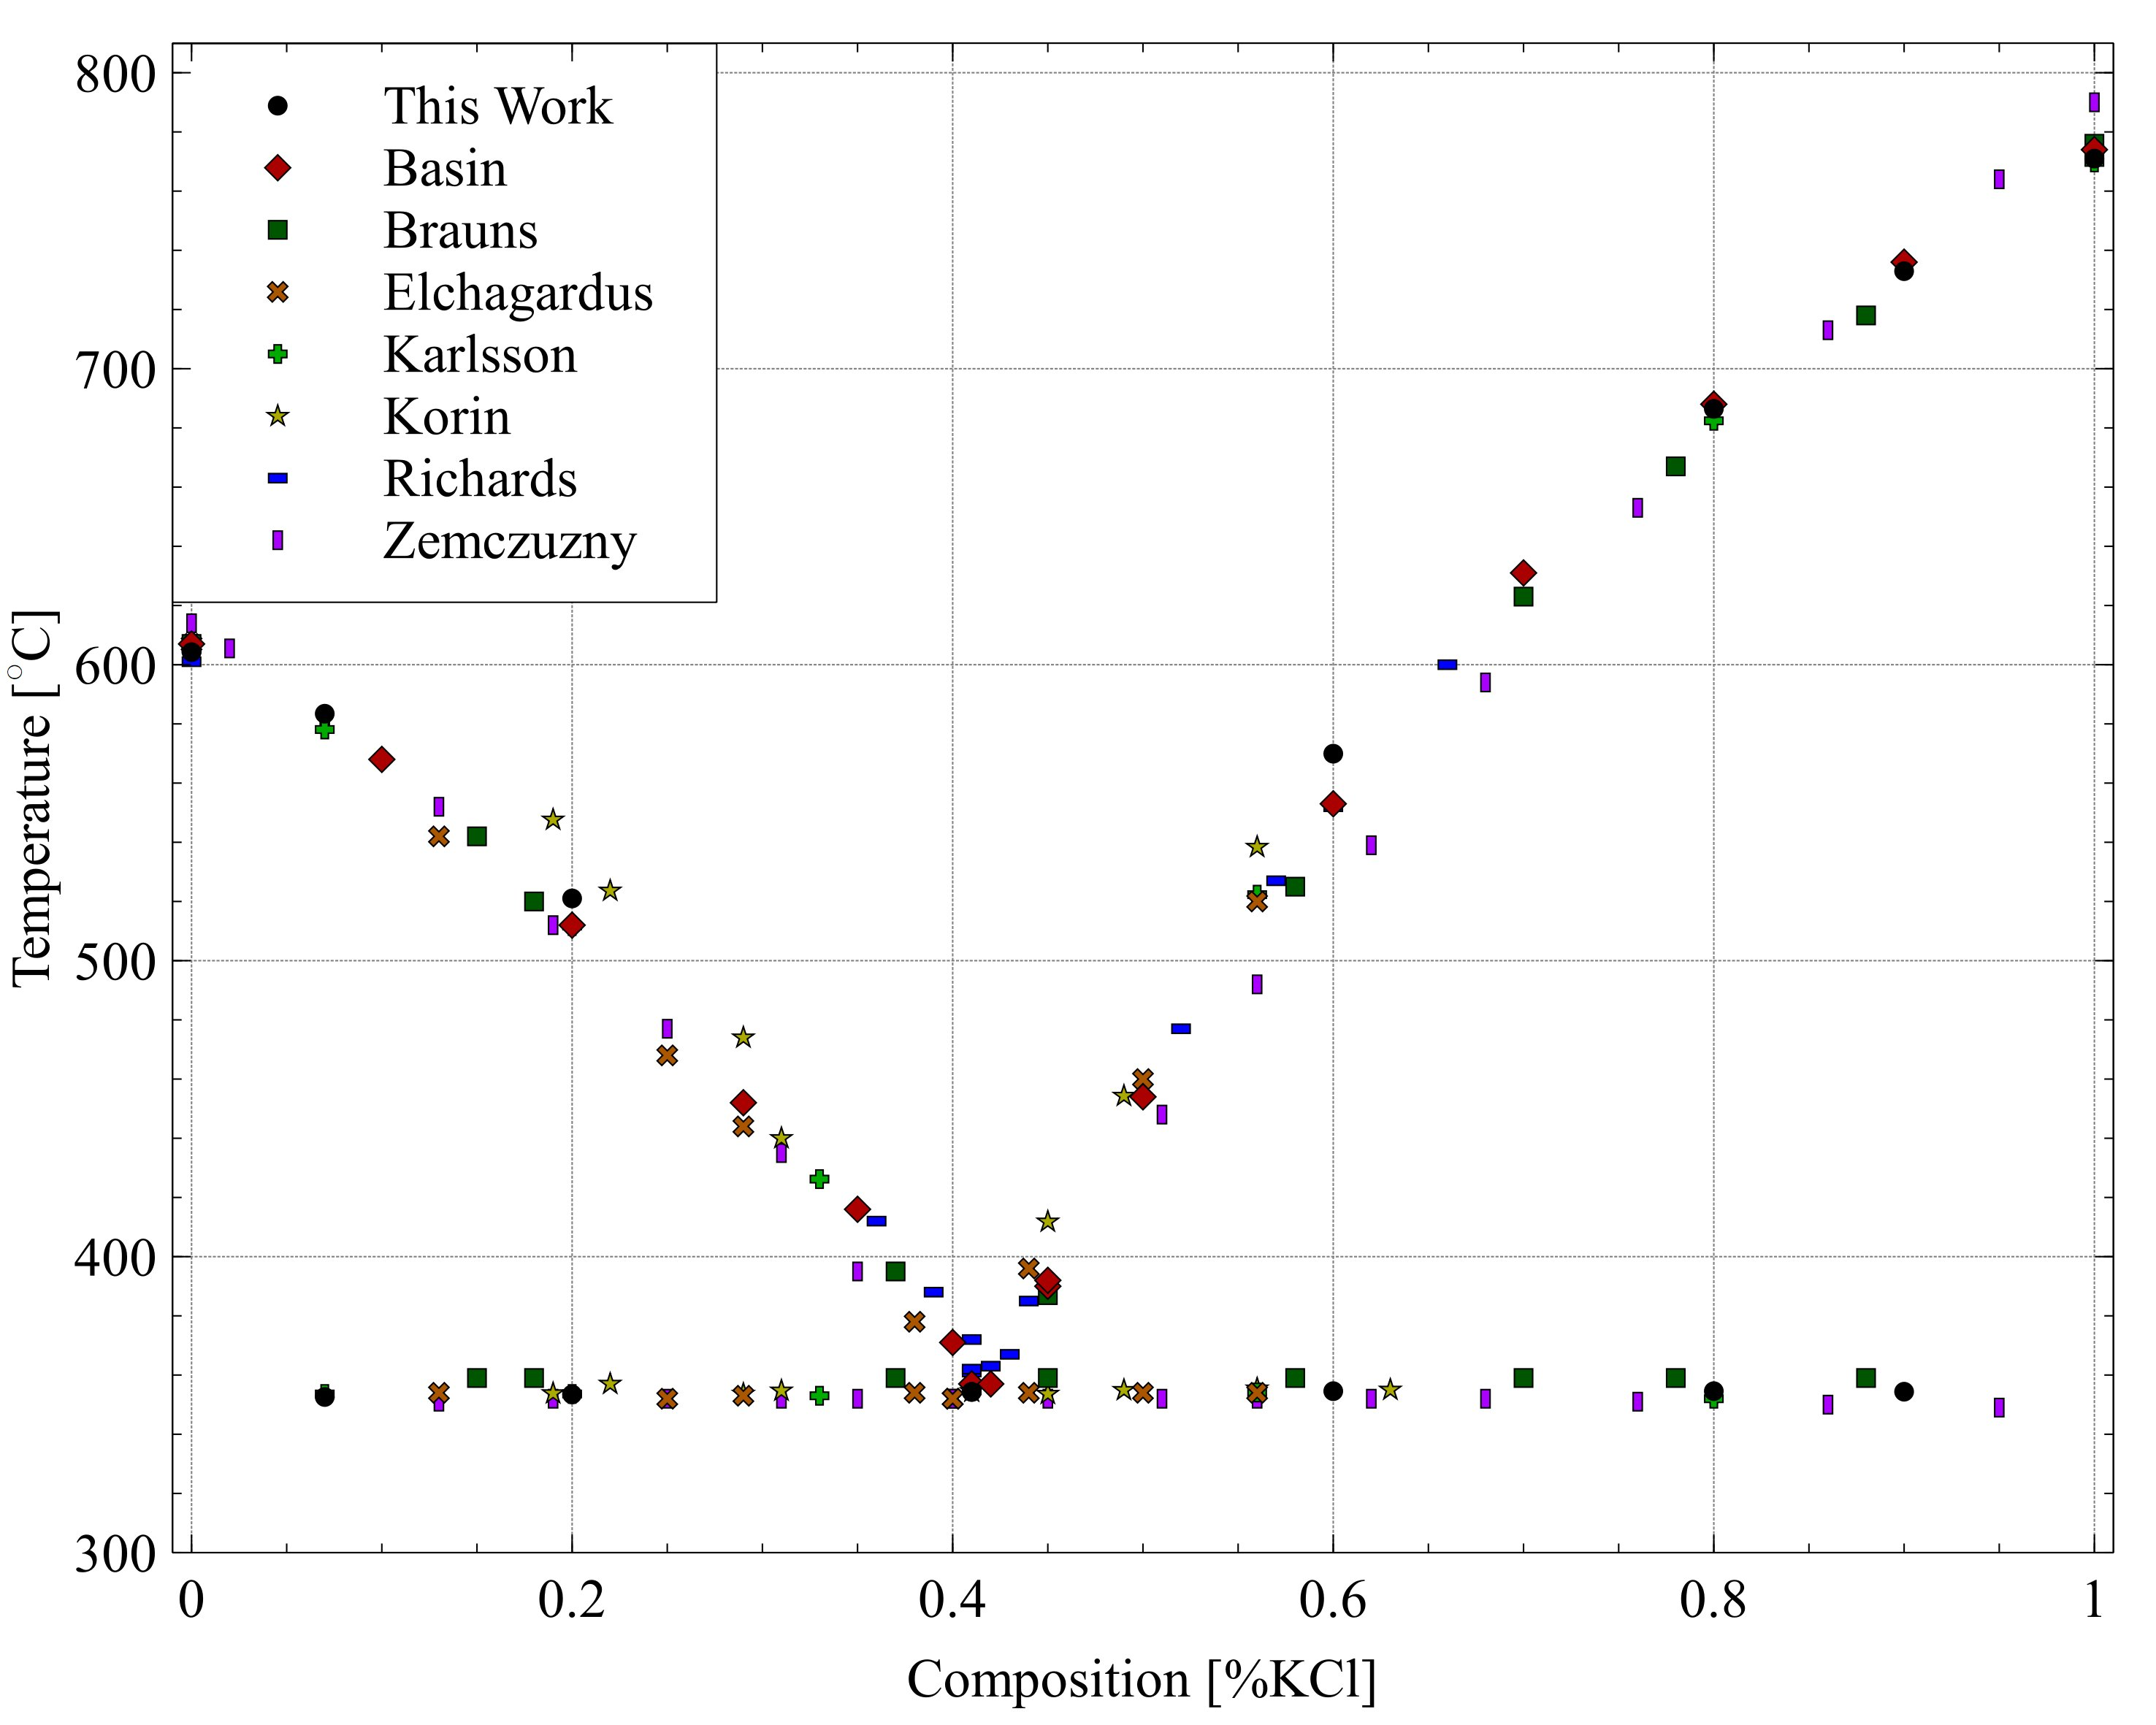
\includegraphics[width=0.7\textwidth]{images/DSC analysis.jpg} 
 \caption{\DIFaddFL{LiCl-KCl binary phase diagram constructed by comparing eutectic and melt temperatures determined from this work to other literature reported values \cite{RN79,RN78,RN77,RN76,RN75,RN16}.}}
 \label{fig:figureDSC}
\end{figure}

 

\begin{figure}[]
 \centering
 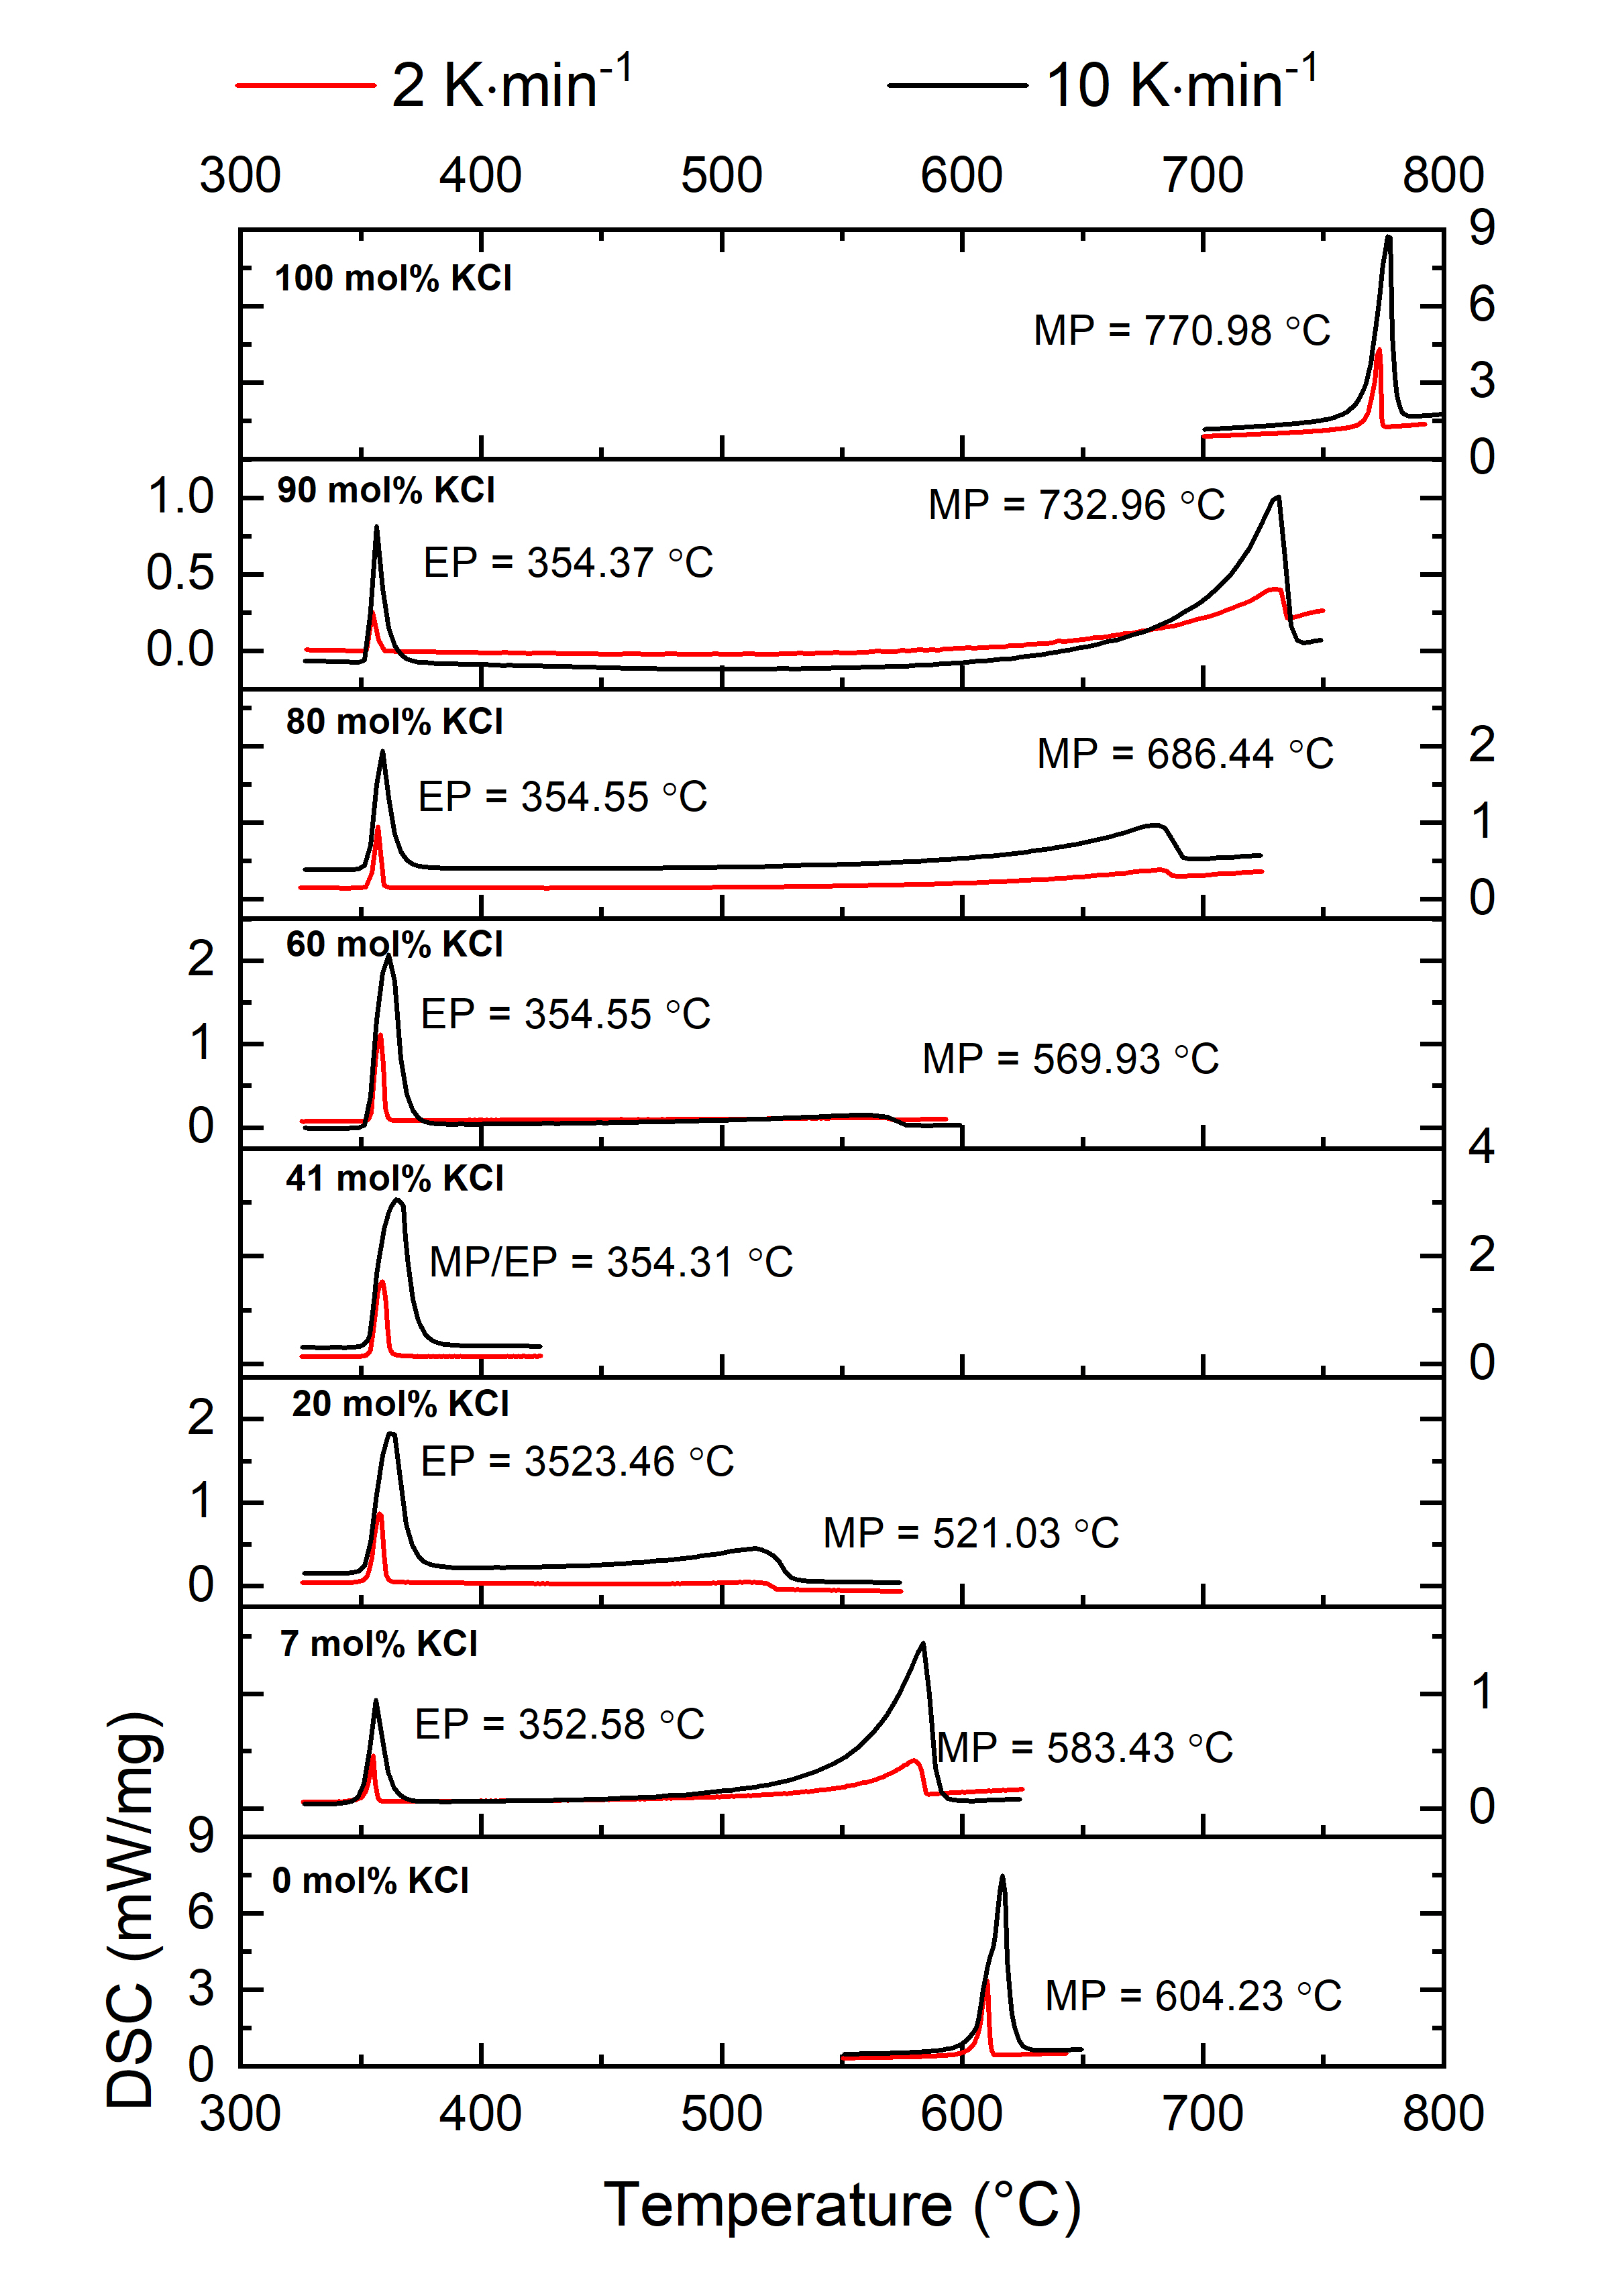
\includegraphics[width=0.7\textwidth]{images/DSCheatcurves.jpg} 
 \caption{\DIFaddFL{Heating curves for each sample studied in the LiCl-KCl binary system. }}
 \label{fig:figureDSC2}
\end{figure}

\FloatBarrier

\DIFaddend \subsection{Comparison of Modeling and Experimental Results}

The experimental densities are extrapolated to \DIFdelbegin \DIFdel{1100 }\DIFdelend \DIFaddbegin \DIFadd{1200 }\DIFaddend K, allowing for direct comparison with previous experimental results in the literature, as well as a comparison to our computational work \DIFdelbegin \DIFdel{(from }\DIFdelend \DIFaddbegin \DIFadd{in }\DIFaddend Fig. \ref{fig:densityCompExp}\DIFdelbegin \DIFdel{)}\DIFdelend . What can be observed is that the computational density matches the experimental data very well, and the experimental data is very similar to the values reported in Janz et al. \DIFdelbegin \DIFdel{\cite{Janz1974}}\DIFdelend \DIFaddbegin \DIFadd{\cite{janz1975molten,van1955electrical}}\DIFaddend . The slight discrepancy between the computational and experimental densities tends to slightly decrease as the concentration nears the eutectic. Fig. \ref{fig:densityCompTemp} illustrates the influence that temperature has on the densities of LiCl, KCl\DIFaddbegin \DIFadd{, }\DIFaddend and the eutectic compositions. What can be observed is that as the composition approaches the eutectic composition the higher the accuracy for density becomes. The average error between the experimental and the computational results for the density of the binary salts LiCl and KCl is 1.42\% and 1.82\%\DIFaddbegin \DIFadd{, }\DIFaddend respectively. The average error at the eutectic composition is 0.96\%. AIMD underpredicts the densities at low temperatures, but this error decreases as the temperature increases and for some compositions overpredicts.


\begin{figure}[h]
 \centering
 \DIFdelbeginFL %DIFDELCMD < 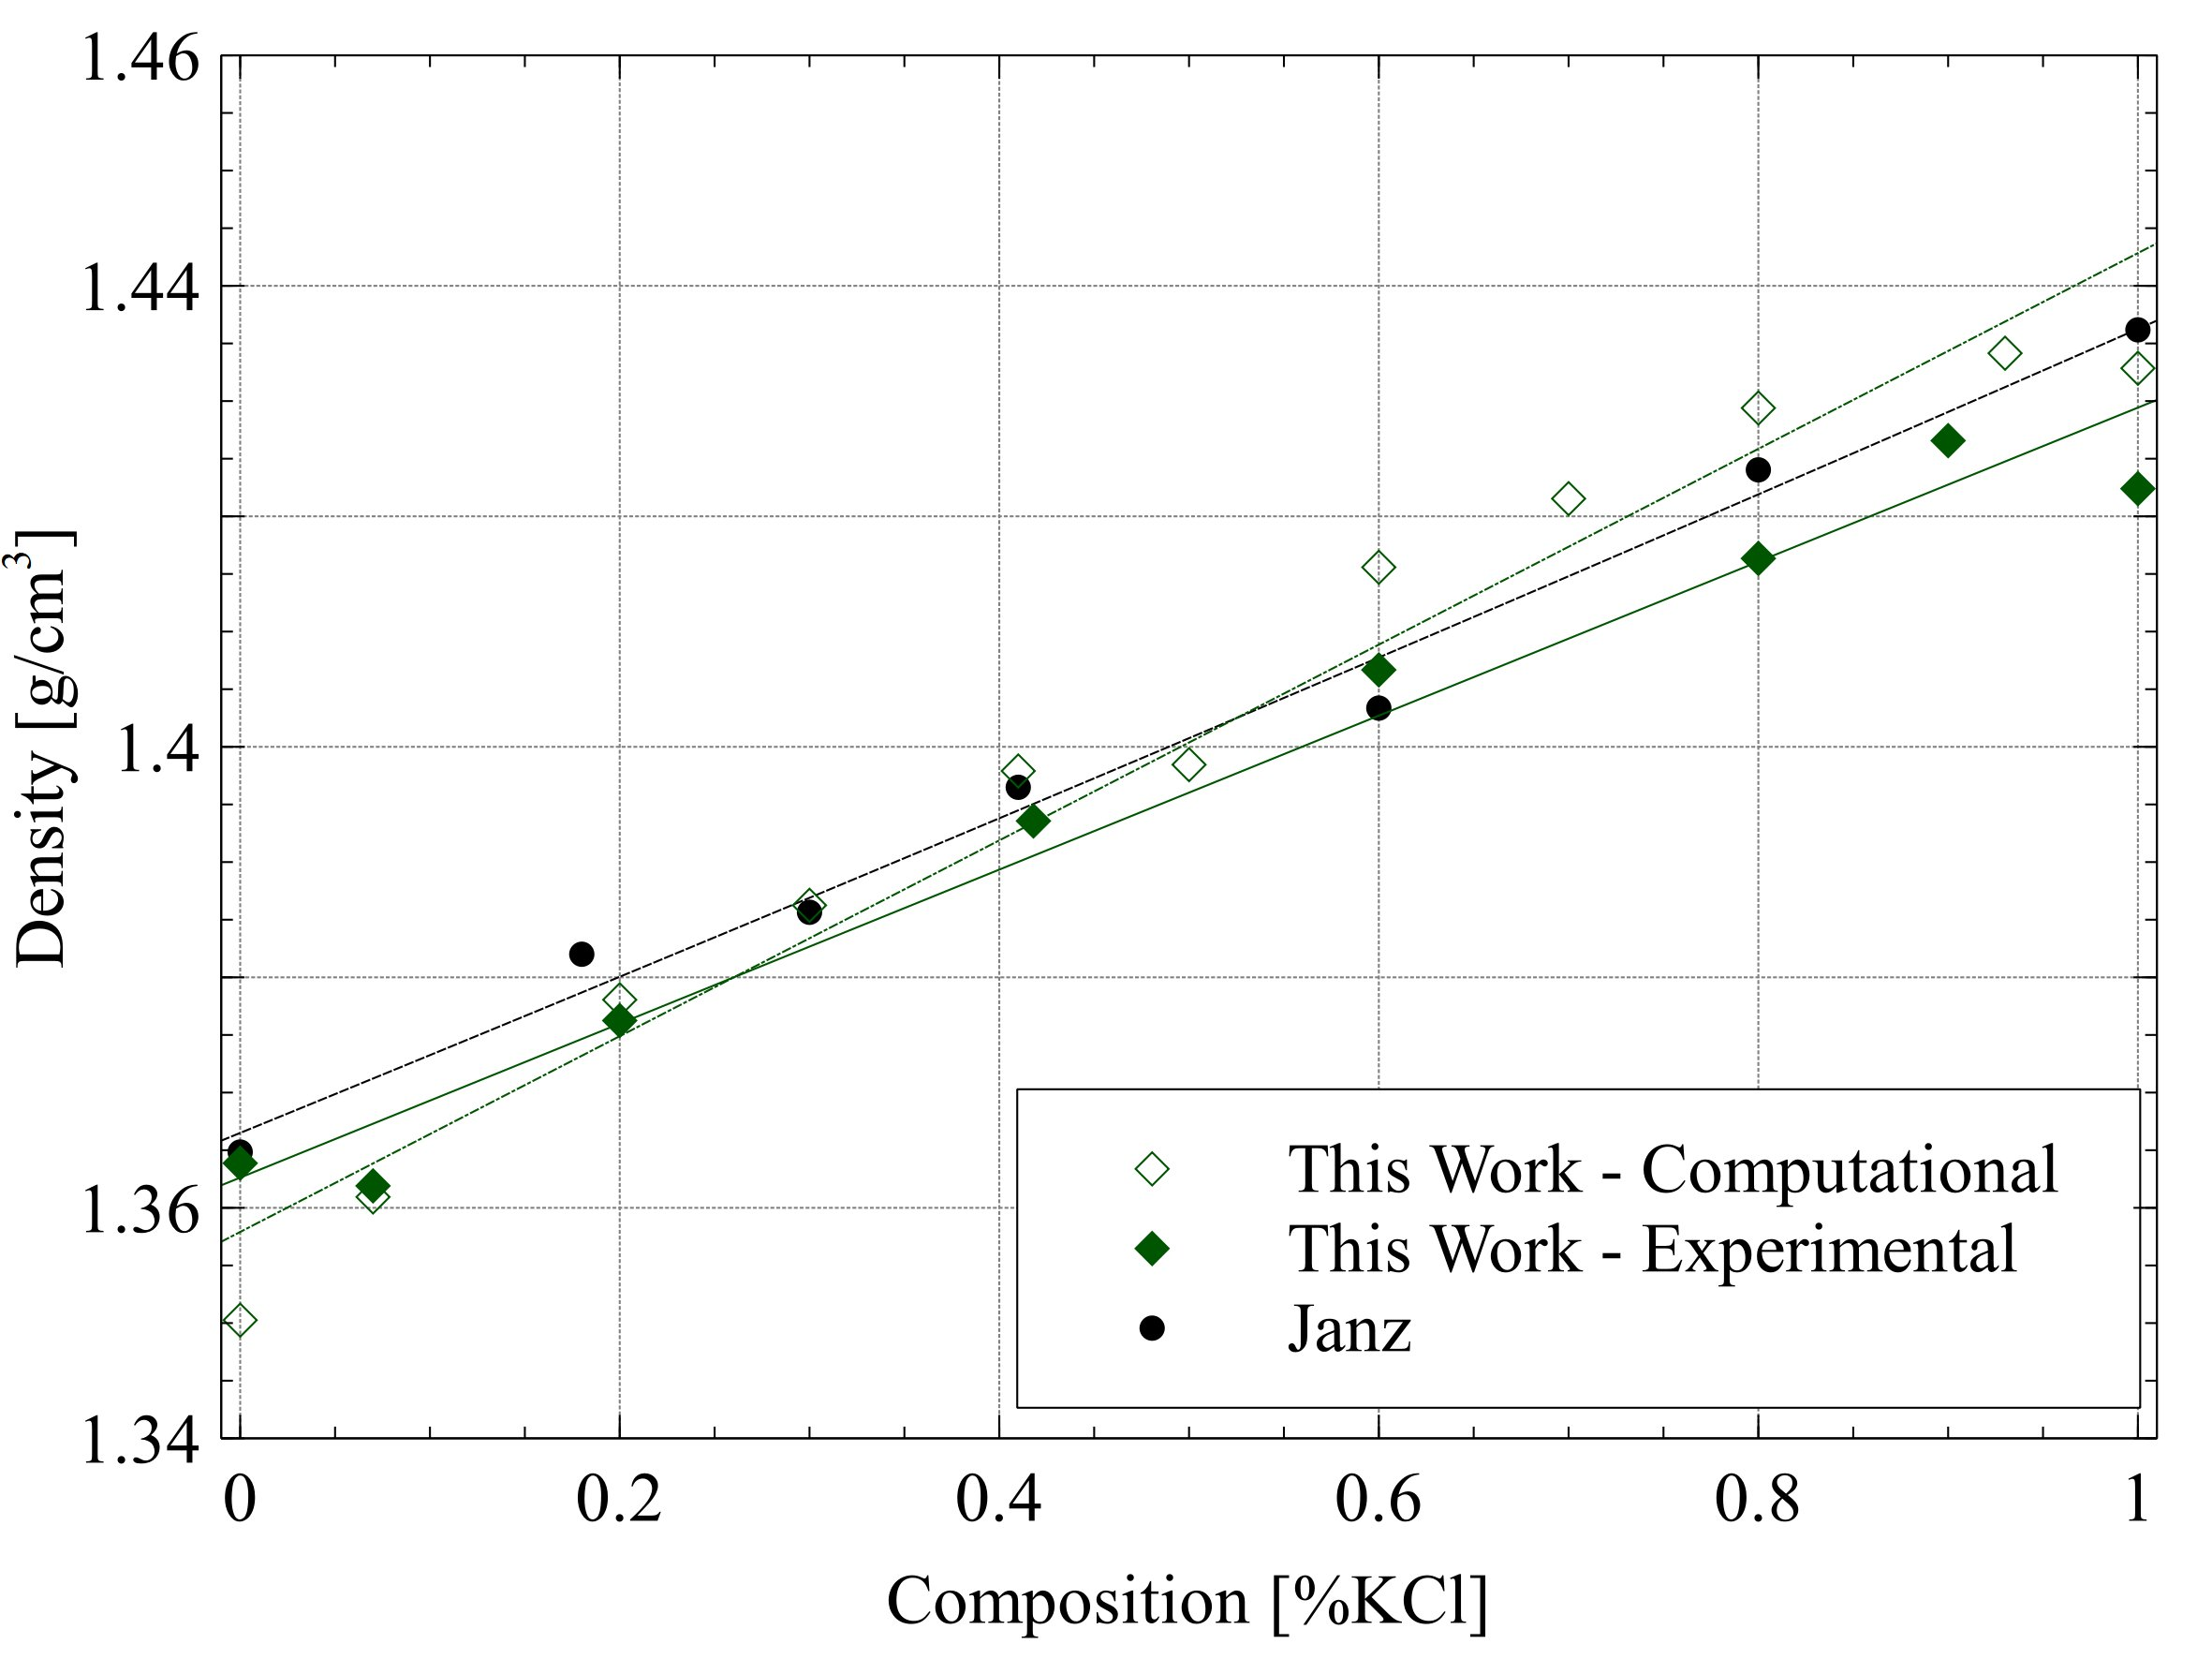
\includegraphics[width=0.8\textwidth]{images/density_comp.jpg} 
%DIFDELCMD <  %%%
\DIFdelendFL \DIFaddbeginFL 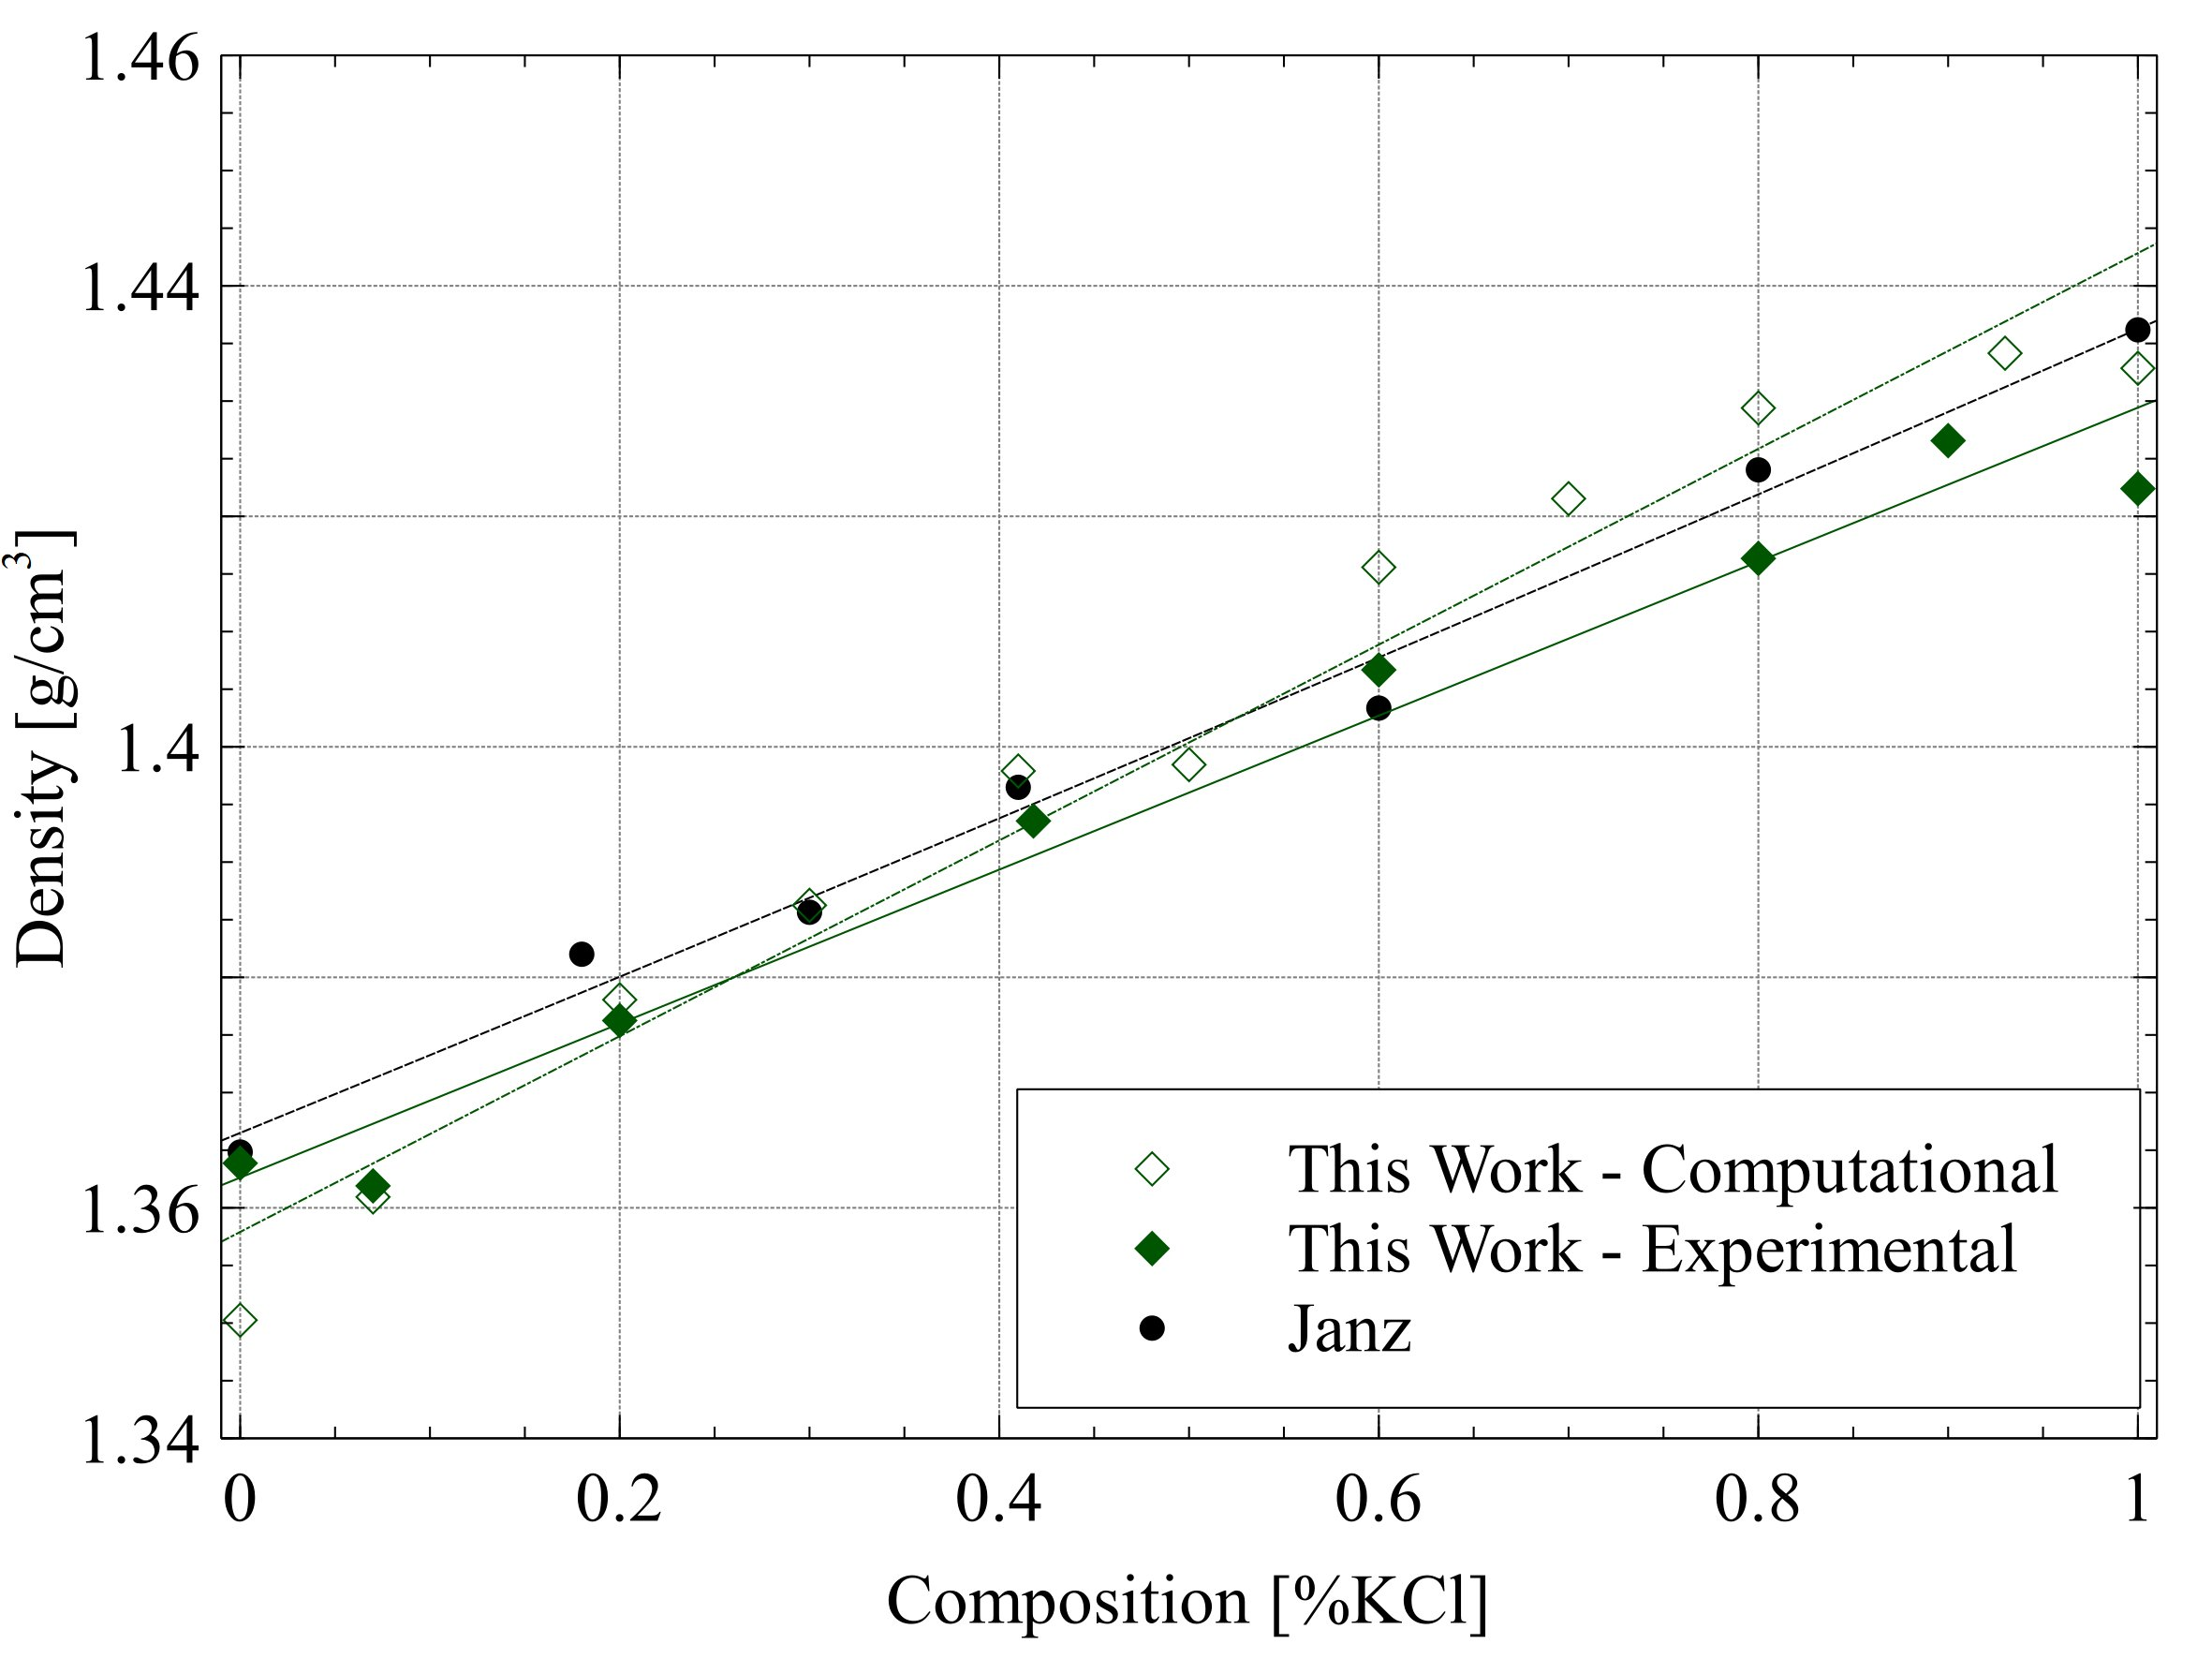
\includegraphics[width=0.7\textwidth]{images/density_comp.jpg} 
 \DIFaddendFL \caption{Density as a function of the composition of LiCl-KCl system at \DIFdelbeginFL \DIFdelFL{1100 }\DIFdelendFL \DIFaddbeginFL \DIFaddFL{1200 }\DIFaddendFL K. Filled markers are experimental and open are computational. AIMD results are compared to the experimental results from \DIFdelbeginFL \DIFdelFL{Wang et al. \cite{Wang2015}, }\DIFdelendFL Janz et al. \DIFdelbeginFL \DIFdelFL{\cite{Janz1988} 1100K}\DIFdelendFL \DIFaddbeginFL \DIFaddFL{\cite{janz1975molten,van1955electrical} 1200K}\DIFaddendFL , and Fig. \ref{fig:density_exp}.}
 \label{fig:densityCompExp}
\end{figure} 


\begin{figure}[h]
 \centering
 \DIFdelbeginFL %DIFDELCMD < 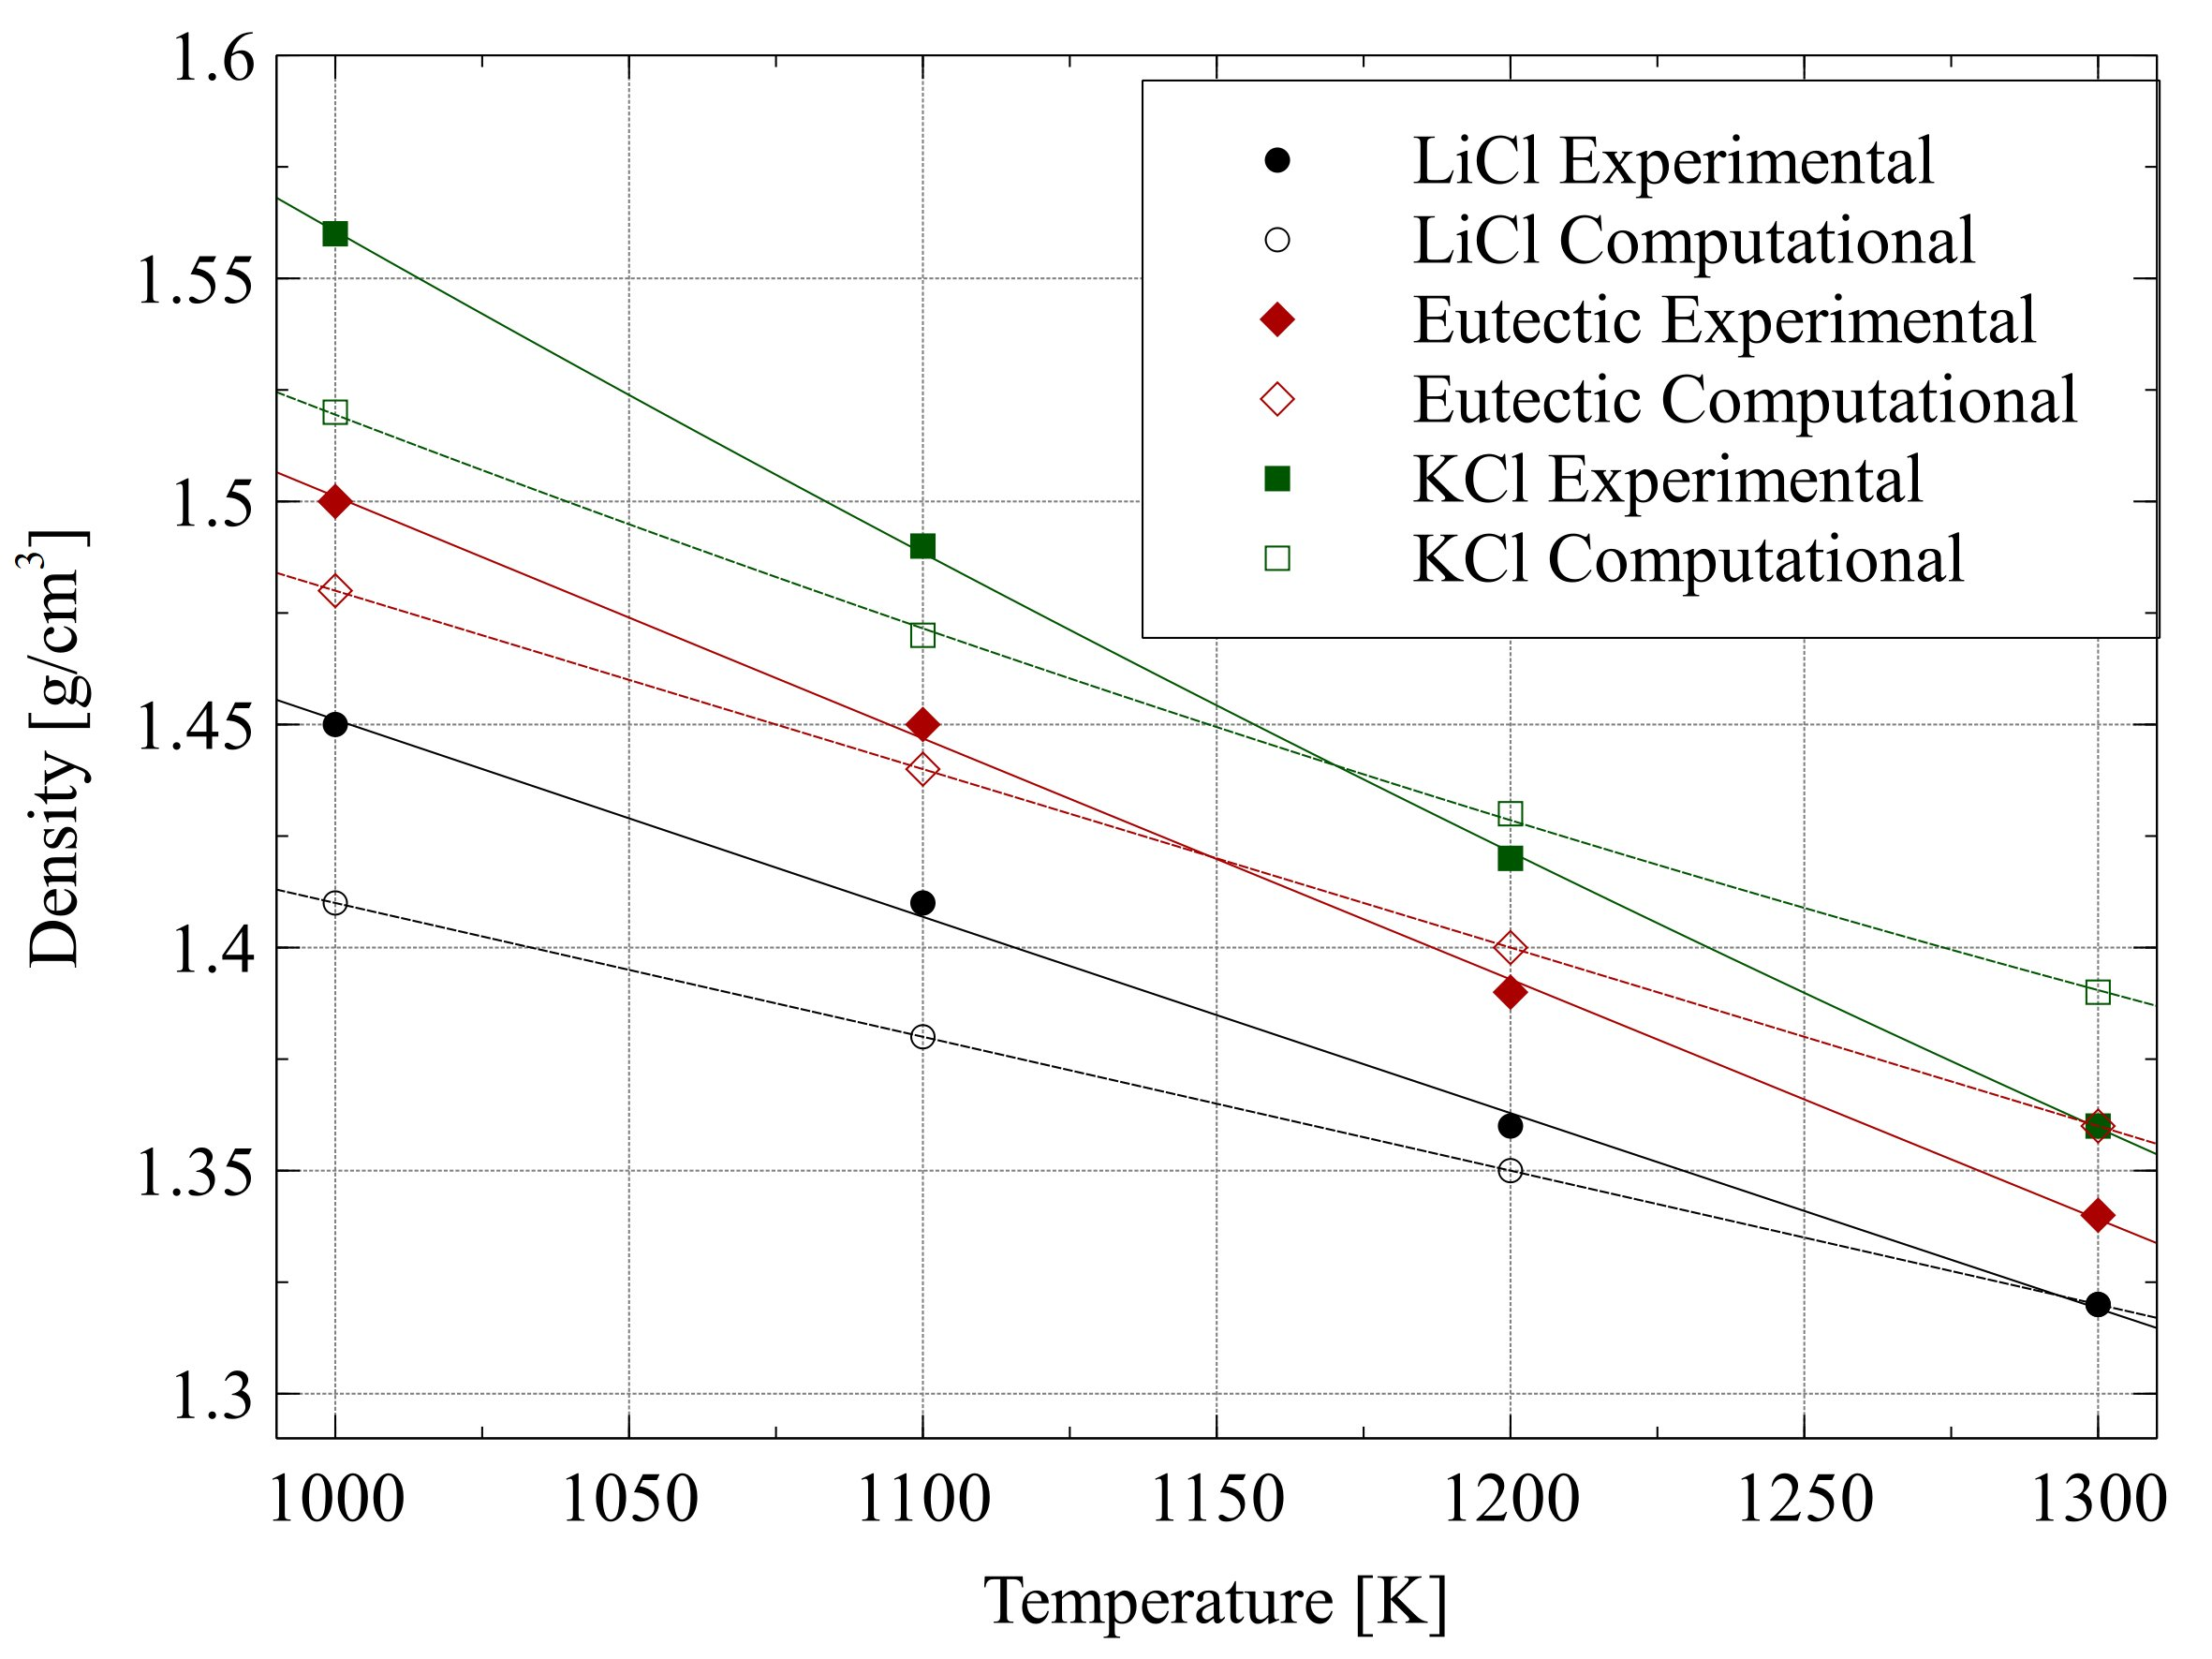
\includegraphics[width=0.8\textwidth]{images/density_temp_comp.jpg} 
%DIFDELCMD <  %%%
\DIFdelendFL \DIFaddbeginFL 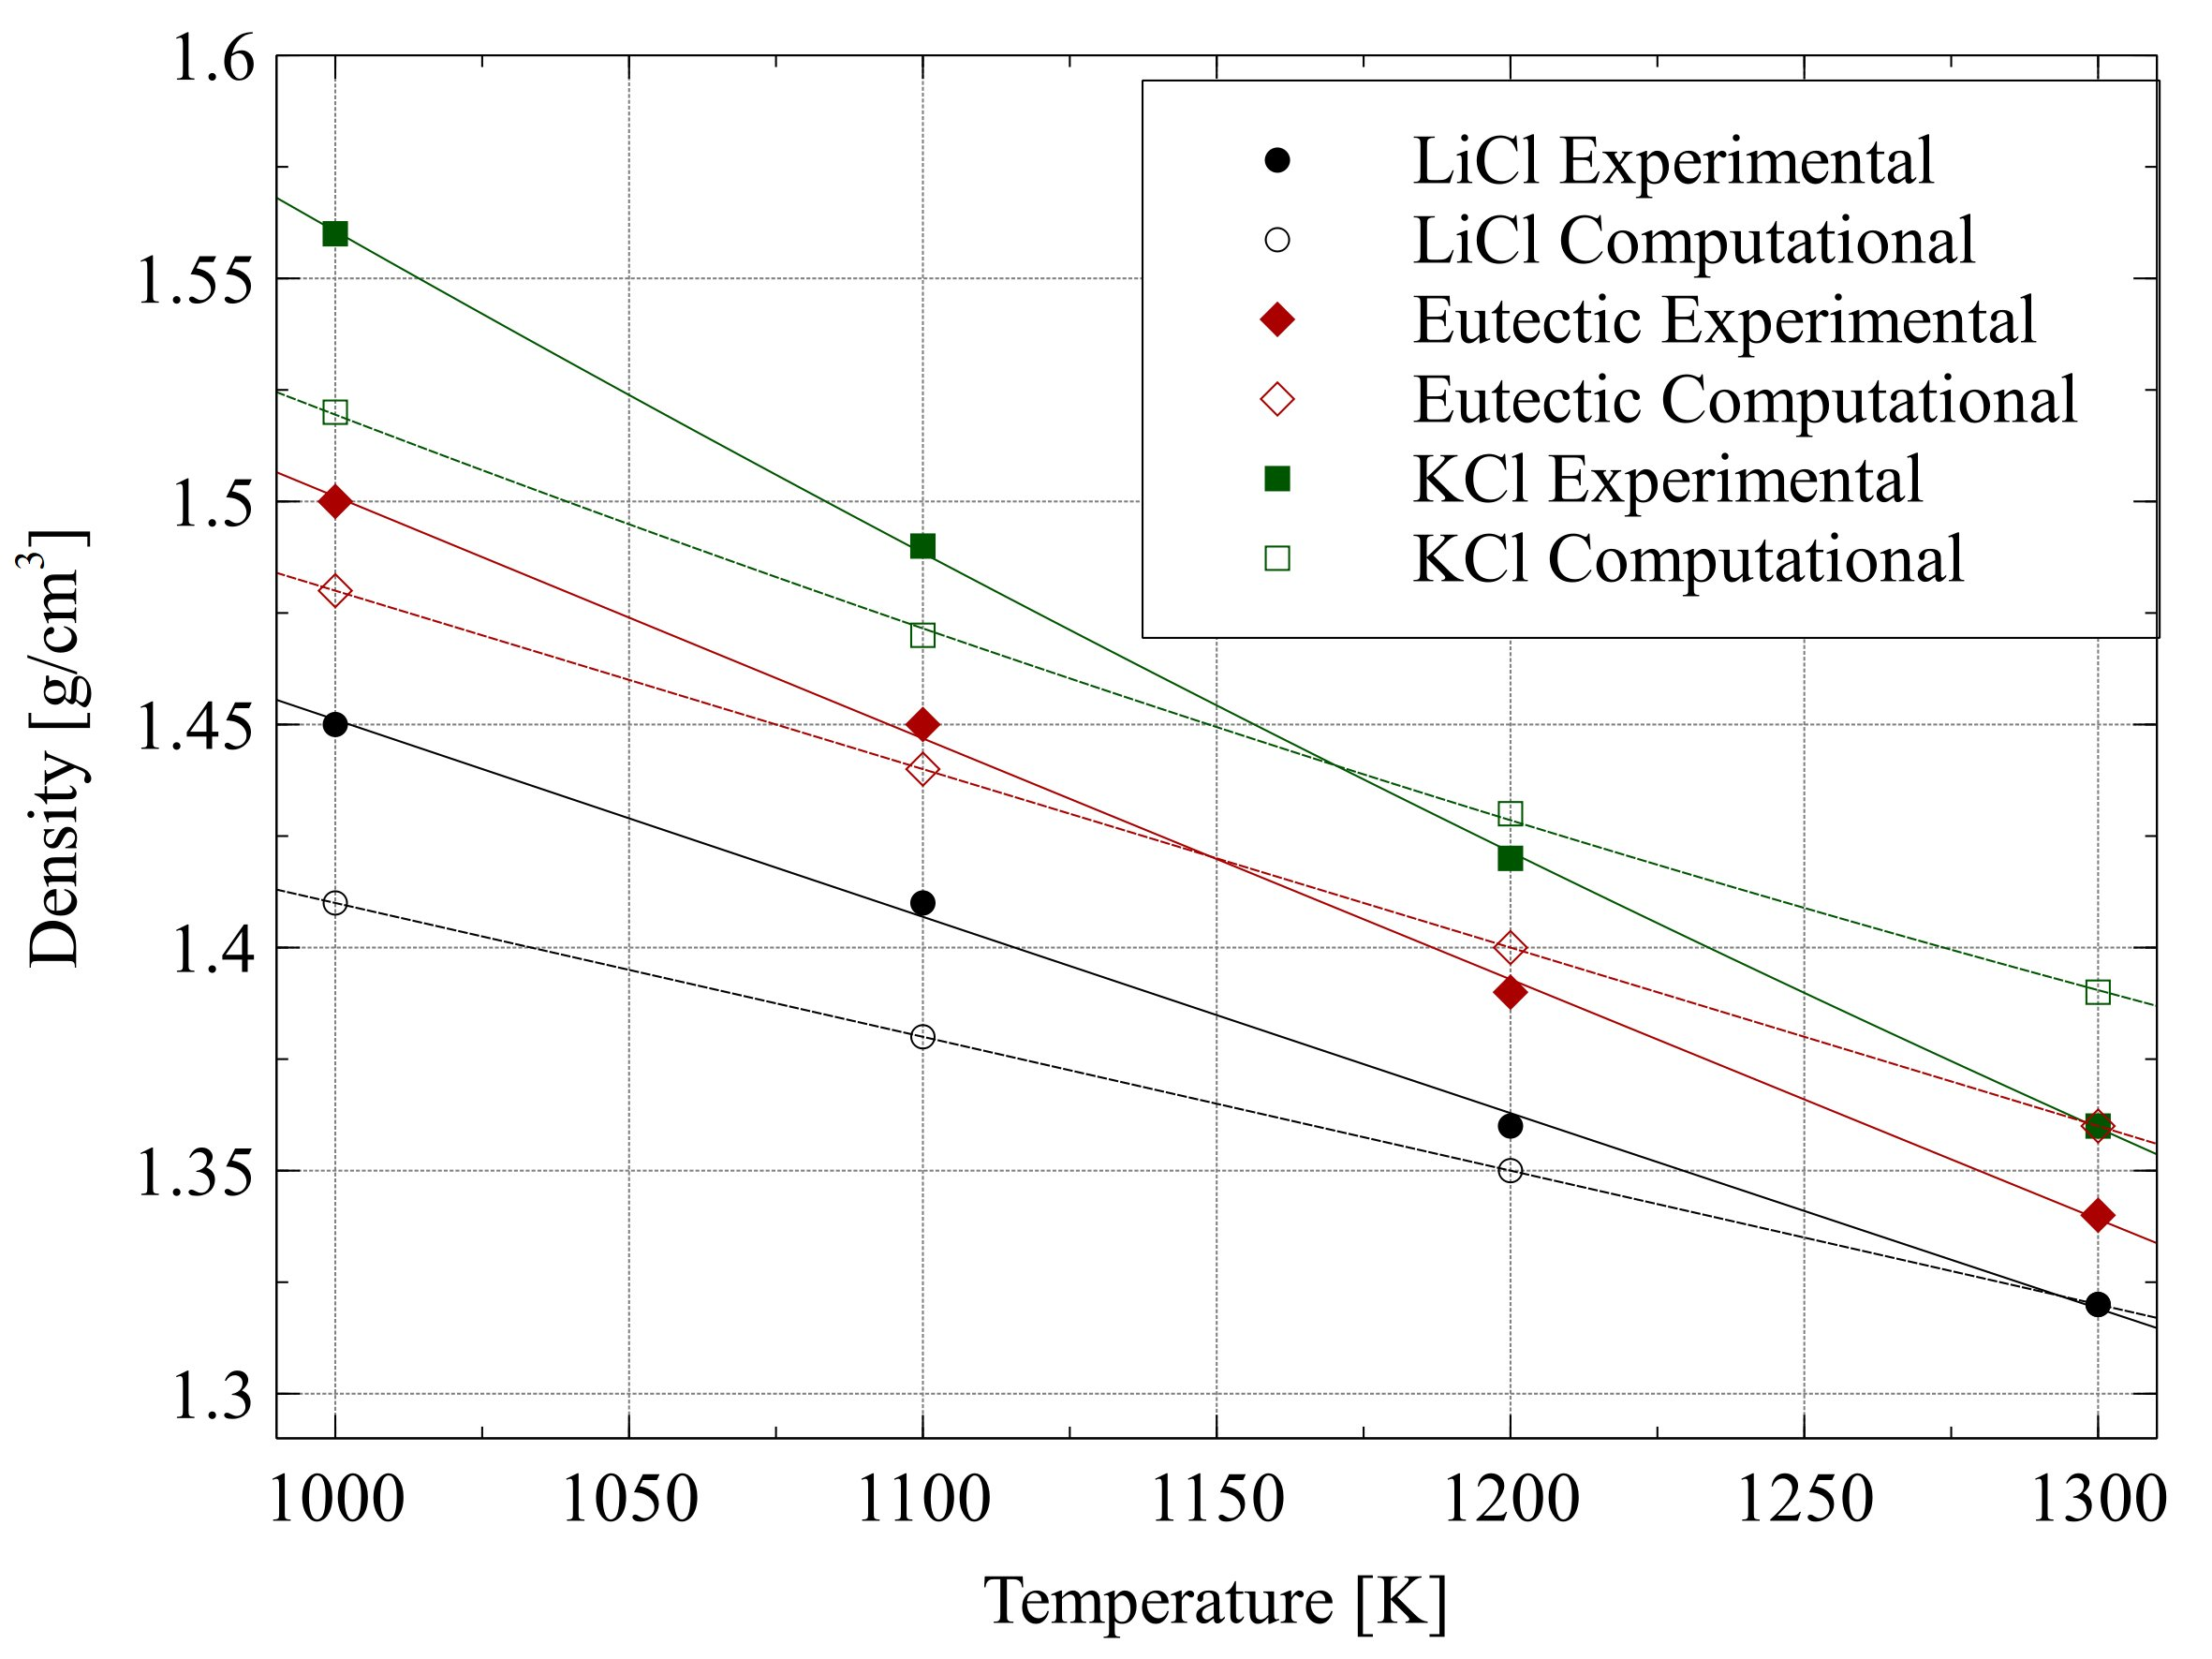
\includegraphics[width=0.7\textwidth]{images/density_temp_comp.jpg} 
 \DIFaddendFL \caption{Density as a function of the temperature for LiCl, eutectic LiCl-KCl, and KCl. Filled markers are experimental and open are computational. Second order polynomial fits to each data set are shown as lines. }
 \label{fig:densityCompTemp}
\end{figure} 
\FloatBarrier

\section{Conclusions}

AIMD simulations were applied to the entire composition range of the LiCl-KCl system in the temperature range 700-1300 K. The properties gathered were density, compressibility, bulk modulus, heat capacity, enthalpy of mixing and Gibbs free energy of mixing. What was observed in this study is that AIMD can be used to calculate the density with an appreciable match with the experimental results. This shows that structural properties can be modeled with AIMD. Heat capacity can be calculated within 8.8\% of experimental values. Values for enthalpy and \DIFdelbegin \DIFdel{Gibb's }\DIFdelend \DIFaddbegin \DIFadd{Gibbs }\DIFaddend free energy of mixing are compared to literature\DIFaddbegin \DIFadd{, are can identify the eutectic composition}\DIFaddend . Compressibility was not \DIFaddbegin \DIFadd{able to be }\DIFaddend compared to experimental values\DIFaddbegin \DIFadd{, }\DIFaddend but were similar to other AIMD studies. This study shows that AIMD can be used to gather a variety of properties without the requirement of \DIFdelbegin \DIFdel{starting from a classical MD run}\DIFdelend \DIFaddbegin \DIFadd{an initial classical MD simulation}\DIFaddend . Values for density were also calculated from experiments of the direct Archimedean method. These values had an appreciable match with \DIFaddbegin \DIFadd{experimental and computational }\DIFaddend literature results for density\DIFaddbegin \DIFadd{, providing a rigorous evaluation of both eutectic, pure, and intermediate compositions in the LiCl-KCl pseudo binary system. Finally, the experimental work served to further confirm the computational results and provide a basis for further computational examination}\DIFaddend .


\section{Acknowledgements}

This material is based upon work supported under an Integrated University Program Graduate Fellowship. This work is also supported through the INL Laboratory Directed Research and Development (LDRD) Program under DOE Idaho Operations Office Contract DE-AC07-05ID14517. This research made use of the resources of the High-Performance Computing Center at Idaho National Laboratory, which is supported by the Office of Nuclear Energy of the U.S. Department of Energy and the Nuclear Science User Facilities.    

\bibliography{reference}
%\end{multicols}

\end{document}a